% Options for packages loaded elsewhere
\PassOptionsToPackage{unicode}{hyperref}
\PassOptionsToPackage{hyphens}{url}
\PassOptionsToPackage{dvipsnames,svgnames,x11names}{xcolor}
%
\documentclass[
  12pt,
  twoside]{article}
\usepackage{amsmath,amssymb}
\usepackage{iftex}
\ifPDFTeX
  \usepackage[T1]{fontenc}
  \usepackage[utf8]{inputenc}
  \usepackage{textcomp} % provide euro and other symbols
\else % if luatex or xetex
  \usepackage{unicode-math} % this also loads fontspec
  \defaultfontfeatures{Scale=MatchLowercase}
  \defaultfontfeatures[\rmfamily]{Ligatures=TeX,Scale=1}
\fi
\usepackage{lmodern}
\ifPDFTeX\else
  % xetex/luatex font selection
\fi
% Use upquote if available, for straight quotes in verbatim environments
\IfFileExists{upquote.sty}{\usepackage{upquote}}{}
\IfFileExists{microtype.sty}{% use microtype if available
  \usepackage[]{microtype}
  \UseMicrotypeSet[protrusion]{basicmath} % disable protrusion for tt fonts
}{}
\makeatletter
\@ifundefined{KOMAClassName}{% if non-KOMA class
  \IfFileExists{parskip.sty}{%
    \usepackage{parskip}
  }{% else
    \setlength{\parindent}{0pt}
    \setlength{\parskip}{6pt plus 2pt minus 1pt}}
}{% if KOMA class
  \KOMAoptions{parskip=half}}
\makeatother
\usepackage{xcolor}
\usepackage[margin = 1in]{geometry}
\usepackage{longtable,booktabs,array}
\usepackage{calc} % for calculating minipage widths
% Correct order of tables after \paragraph or \subparagraph
\usepackage{etoolbox}
\makeatletter
\patchcmd\longtable{\par}{\if@noskipsec\mbox{}\fi\par}{}{}
\makeatother
% Allow footnotes in longtable head/foot
\IfFileExists{footnotehyper.sty}{\usepackage{footnotehyper}}{\usepackage{footnote}}
\makesavenoteenv{longtable}
\usepackage{graphicx}
\makeatletter
\def\maxwidth{\ifdim\Gin@nat@width>\linewidth\linewidth\else\Gin@nat@width\fi}
\def\maxheight{\ifdim\Gin@nat@height>\textheight\textheight\else\Gin@nat@height\fi}
\makeatother
% Scale images if necessary, so that they will not overflow the page
% margins by default, and it is still possible to overwrite the defaults
% using explicit options in \includegraphics[width, height, ...]{}
\setkeys{Gin}{width=\maxwidth,height=\maxheight,keepaspectratio}
% Set default figure placement to htbp
\makeatletter
\def\fps@figure{htbp}
\makeatother
\setlength{\emergencystretch}{3em} % prevent overfull lines
\providecommand{\tightlist}{%
  \setlength{\itemsep}{0pt}\setlength{\parskip}{0pt}}
\setcounter{secnumdepth}{5}
\newlength{\cslhangindent}
\setlength{\cslhangindent}{1.5em}
\newlength{\csllabelwidth}
\setlength{\csllabelwidth}{3em}
\newlength{\cslentryspacingunit} % times entry-spacing
\setlength{\cslentryspacingunit}{\parskip}
\newenvironment{CSLReferences}[2] % #1 hanging-ident, #2 entry spacing
 {% don't indent paragraphs
  \setlength{\parindent}{0pt}
  % turn on hanging indent if param 1 is 1
  \ifodd #1
  \let\oldpar\par
  \def\par{\hangindent=\cslhangindent\oldpar}
  \fi
  % set entry spacing
  \setlength{\parskip}{#2\cslentryspacingunit}
 }%
 {}
\usepackage{calc}
\newcommand{\CSLBlock}[1]{#1\hfill\break}
\newcommand{\CSLLeftMargin}[1]{\parbox[t]{\csllabelwidth}{#1}}
\newcommand{\CSLRightInline}[1]{\parbox[t]{\linewidth - \csllabelwidth}{#1}\break}
\newcommand{\CSLIndent}[1]{\hspace{\cslhangindent}#1}
\usepackage{placeins}
\usepackage{setspace}
\usepackage{microtype}
\usepackage{indentfirst}
\usepackage{tipa}
\usepackage{float}
\usepackage{hyperref}
\doublespacing
\counterwithin{figure}{section}
\counterwithin{table}{section}
\setlength{\headheight}{14.5pt}
\setlength{\parskip}{0cm}
\setlength\parindent{24pt}
\raggedbottom
\usepackage{booktabs}
\usepackage{longtable}
\usepackage{array}
\usepackage{multirow}
\usepackage{wrapfig}
\usepackage{float}
\usepackage{colortbl}
\usepackage{pdflscape}
\usepackage{tabu}
\usepackage{threeparttable}
\usepackage{threeparttablex}
\usepackage[normalem]{ulem}
\usepackage{makecell}
\usepackage{xcolor}
\ifLuaTeX
  \usepackage{selnolig}  % disable illegal ligatures
\fi
\IfFileExists{bookmark.sty}{\usepackage{bookmark}}{\usepackage{hyperref}}
\IfFileExists{xurl.sty}{\usepackage{xurl}}{} % add URL line breaks if available
\urlstyle{same}
\hypersetup{
  colorlinks=true,
  linkcolor={black},
  filecolor={Maroon},
  citecolor={Blue},
  urlcolor={black},
  pdfcreator={LaTeX via pandoc}}

\author{}
\date{\vspace{-2.5em}}

\begin{document}

\pagenumbering{roman}
\thispagestyle{empty}

\begin{centering}

The Pennsylvania State University\\
The Graduate School

\vspace{3 cm}

\MakeUppercase{\bf Cross-language transfer in voice onset time: A window into perceptual adaptation in brain and behavior}

\vspace{3 cm}

A Dissertation in\\
Psychology\\
by\\
Holly A. Zaharchuk

\vspace{1.5 cm}

\copyright 2024 Holly A. Zaharchuk

\vspace{1.5 cm}

Submitted in Partial Fulfillment\\
of the Requirements\\
for the Degree of\\

\vspace{0.75 cm}

Doctor of Philosophy

\vspace{0.75 cm}

August 2024

\end{centering}

\newpage

\begin{flushleft}
\begin{singlespacing}

The dissertation of Holly A. Zaharchuk was reviewed and approved by the following:\\

\vspace{12pt}

Janet G. van Hell\\
Professor of Psychology and Linguistics\\
Dissertation Advisor\\
Chair of Committee\\

\vspace{12pt}

Michele T. Diaz\\
Professor of Psychology and Linguistics\\

\vspace{12pt}

Navin Viswanathan\\
Associate Professor of Communication Sciences and Disorders and Linguistics\\

\vspace{12pt}

Matthew Carlson\\
Associate Professor of Spanish and Linguistics\\

\vspace{12pt}

Kristin A. Buss\\
Professor of Psychology and Human Development and Family Studies\\
Head of the Department of Psychology\\

\end{singlespacing}
\end{flushleft}

\newpage
\section*{Abstract}

Cross-language transfer from L1 Spanish to L2 English during speech production can create ambiguity between the voiceless stops /p/, /t/, and /k/ and their voiced counterparts /b/, /d/, and /g/ during speech perception.
This perceptual ambiguity between voiced and voiceless stop pairs is a result of their voice onset time (VOT) distributions.
Specifically, Spanish-accented English talkers tend to produce short lag VOTs for voiceless stops, while L1 English listeners tend to associate short lag VOTs with voiced stops.
This dissertation features two studies that explore different aspects of adaptation to Spanish-accented English voiceless stops.
Overall, stop VOT provides a window into the process of adapting to L2-accented speech in behavior (Study 1) and the brain (Study 2).

Study 1 investigated the structure and content of exposure to L2-accented speech in talker-independent adaptation.
There are two competing explanations for how perceptual learning can transfer from one talker to another.
The exposure-to-variability hypothesis argues that increasing covariation between acoustic-phonetic cues during exposure increases performance on a new talker.
The similarity-based hypothesis argues that increasing cue-category overlap between the exposure and test talkers increases performance on the test talker.
To compare these hypotheses, a series of three experiments was conducted with a novel experimental approach that improved the scope and precision of operationalizing variability and similarity compared to previous studies.
Performance on a novel Spanish-accented English talker was measured after exposure to three different Spanish-accented English talkers.
Increasing the similarity between exposure and test facilitated generalization, but only when variability was constrained.
These results provide the strongest support for the similarity-based hypothesis.

Study 2 investigated the relative contributions of acoustic-phonetic and lexico-semantic levels of processing to talker-specific perceptual adaptation.
While behavioral paradigms consistently exhibit rapid improvements in performance with exposure to L2-accented talkers, the effects of perceptual adaptation on neural signatures are less clear.
To clarify previous findings and bring them in line with the behavioral literature, an EEG experiment was conducted that exposed listeners to a Spanish-accented talker's VOT-voiceless stop mappings.
Listeners gained experience with ambiguous onsets in the context of multisyllabic real words like \emph{passage}.
The status of the adaptation process was probed with monosyllabic real words like \emph{park}.
Changes in processing the ambiguous monosyllabic words were investigated as a function of systematic exposure to the unambiguous multisyllabic words in a primed cross-modal go/no-go lexical decision task.
Differences in VOT encoding were observed on the N1 and in phonetic categorization on the P2, which emerged as differences in priming on the N400 disappeared.
These results suggest that changes in acoustic-phonetic representations drive adaptation.

\renewcommand{\contentsname}{Table of contents}

\newpage
\setcounter{tocdepth}{3}
\tableofcontents

\clearpage
\phantomsection
\addcontentsline{toc}{section}{List of figures}
\listoffigures

\clearpage
\phantomsection
\addcontentsline{toc}{section}{List of tables}
\listoftables

\clearpage
\section*{Acknowledgements}
\addcontentsline{toc}{section}{Acknowledgements}

This project would not have been possible without the support of many.
First, my advisor and committee chair, Janet, has my enduring gratitude for her mentorship.
Through countless discussions, late-night emails, and rounds of editing, she worked tirelessly to guide me through the process of developing, implementing, and writing this dissertation.
Her infectious enthusiasm for language science continues to nurture the intellectual curiosity that brought me to Penn State six years ago.
Second, I am grateful for the encouragement and patience of my committee.
I am indebted not only to Michele for her invaluable feedback and guidance throughout my PhD, but also to Navin and Matt for stepping in to provide their expertise in the new (to me) research areas that I explored in this project.
Finally, this work was supported by a National Science Foundation Linguistics Program Doctoral Dissertation Research Improvement Grant (NSF Ling-DDRI: BCS-2234907), Pennsylvania State University Graduate Fellowship (UGF), and Center for Language Science Adele Miccio Memorial Travel Award to visit Dr.~Emily Myers at the University of Connecticut.
The findings and conclusions do not necessarily reflect the views of the funding agencies.

I would also be remiss not to thank my friends and family.
To start, I am so grateful for my lab- and cohort-mates Abby, Adri, Cristal, Eric, and Daisy.
From trips to the grocery store to trips across the ocean, your friendship has been a constant source of comfort and support throughout the last six years.
To my DC girlies Arshia, Mariama, Mary Kate, Sarah Jane, Tor, and Worthy: I feel so lucky to have such an intelligent, caring, and elusive/exclusive group of women in my corner.
I am forever grateful for your love and encouragement.
Finally, to my family, thank you for believing in me always.
A mi querido, te agradezco por apoyarme, cuidarme, y, por supuesto, alimentarme.

\newpage
\pagenumbering{arabic}

\hypertarget{general-introduction}{%
\section{General introduction}\label{general-introduction}}

Of all the world's languages, English has both the largest number of speakers and the broadest geographic reach (Ethnologue, 2024).
Approximately 1.1 billion English speakers, comprising 75\% of the English-speaking population, learned English as a second language (L2).
To the extent that L1 phonetic features transfer to an L2, L2-accented varieties of English are ubiquitous.
From a listener's perspective, L2-accented varieties differ from L1-accented varieties in ways that complicate speech perception.
Nevertheless, listeners show remarkable speed and plasticity in adjusting to L2-accented speech (e.g., Clarke \& Garrett, 2004; Xie et al., 2018).
It remains unclear, however, what underlying mechanisms drive these rapid adaptation effects.
Understanding flexibility in spoken language processing is critical for informing linguistic theories of speech perception (e.g., Kleinschmidt, 2019).
To that end, the present dissertation features two studies, reported in Chapters 2 and 3, exploring the interface between L2 speech production and L1 speech perception.

\hypertarget{cross-language-influence-in-l2-speech-production}{%
\subsection{Cross-language influence in L2 speech production}\label{cross-language-influence-in-l2-speech-production}}

During L2 acquisition, a speaker's L1 phonetic inventory shapes the production of L2 speech sounds (Flege \& Bohn, 2021; for a recent review, see Nagle \& Baese-Berk, 2022).
This cross-language influence in bilingual speech production is a product of the relations between L1 and L2 phonetic categories (Flege et al., 2003; Flege, 2007).
These relations determine how an L2 phone is categorized within the L1 phonological system (Best et al., 2001; Best \& Tyler, 2007).
In this thesis, I focus on two-category assimilation (Best, 1994; Tyler et al., 2014), where two contrasting L2 phonemes map onto two contrasting L1 phonemes.
Specifically, I focus on the three pairs of phonemes found in English, Spanish, and many other languages, which contrast in terms of voicing: /p/-/b/ (\emph{park} vs.~\emph{bark}), /t/-/d/ (\emph{tune} vs.~\emph{dune}), and /k/-/g/ (\emph{coal} vs.~\emph{goal}).
These voicing contrasts form the basis of the experimental manipulations in this dissertation.

\hypertarget{english-stop-consonant-production}{%
\subsubsection{English stop consonant production}\label{english-stop-consonant-production}}

Voicing refers to the status of the glottis, which comprises two folds of tissue and is located in the larynx at the top of the neck.
Constricting the vocal folds causes them to vibrate, resulting in voiced speech sounds.
By contrast, opening the vocal folds prevents vocal fold vibration, resulting in voiceless speech sounds.
The consonants /p/, /t/, and /k/ are voiceless, while the consonants /b/, /d/, and /g/ are voiced.

We can further describe these six speech sounds by where and how they are produced in the vocal tract (i.e., the structures in the upper neck and head that are used for speech).
First, each pair of consonants is grouped according to where in the vocal tract it is produced, referred to as the place of articulation: bilabial consonants are produced with the lips (/p/-/b/), alveolar consonants are produced with the tongue at the roof of the mouth just behind the teeth (i.e., the alveolar ridge; /t/-/d/), and velar consonants are produced with the tongue at the soft palate in the back of the mouth (i.e., the velum; /k/-/g/).
The lips, tongue, alveolar ridge, and velum are all instances of articulators.
Second, all six of these consonants are grouped together according to the manner of articulation, which is how a sound is produced in the vocal tract.
A stop consonant, also referred to as a plosive, is characterized by a complete closure of the vocal tract at the relevant place of articulation.
This is distinguished from a fricative, which is characterized by a partial closure of the vocal tract, creating vibration at the relevant place of articulation (e.g., /f/, /s/, and /\textipa{S}/).

To summarize, the consonant pairs /p/-/b/, /t/-/d/, and /k/-/g/ all have the same manner of articulation (stop) but have different places of articulation (bilabial, alveolar, and velar, respectively).
Within each pair, one member differs from the other in terms of voicing (voiceless-voiced, respectively).
While this small articulatory distinction plays a big role in the phonological systems of many languages, including English and Spanish, it can be difficult to detect in continuous speech where the acoustic-phonetic dynamics are complex.
Throughout language acquisition, listeners (and speakers themselves) learn which acoustic-phonetic features are most strongly associated with these fine-grained phonological voicing distinctions.
There are several interrelated cues that listeners use to distinguish voiced from voiceless stops in word-initial position, including onset fundamental frequency (Whalen et al., 1993), formant transitions (Benkí, 2001; Cooper, 1974), and vowel duration (Port \& Dalby, 1982; Viswanathan et al., 2020).
However, the primary cue to word-initial stop consonant voicing is voice onset time (VOT), which is the interval between the release of the closure of the articulators, called the burst, and the beginning of voicing (Cho \& Ladefoged, 1999; Chodroff et al., 2019; Lisker \& Abramson, 1964).
Listeners are highly sensitive to the probabilistic distributions of VOT across voiced and voiceless English stops (Clayards et al., 2008).

\hypertarget{spanish-to-english-transfer-in-vot-production}{%
\subsubsection{Spanish-to-English transfer in VOT production}\label{spanish-to-english-transfer-in-vot-production}}

The associations between VOT and stop consonants vary cross-linguistically (Chodroff et al., 2019; Lisker \& Abramson, 1970).
There are three general types of VOT: lead, where voicing begins before the release, resulting in negative values; short lag, where voicing begins immediately or relatively quickly after the release; and long lag, where voicing begins relatively slowly after the release (Abramson \& Whalen, 2017).
In Spanish, lead VOTs correspond to voiced stops and short lag VOTs correspond to voiceless stops (Vicente, 1986; Williams, 1977).
For example, the /b/ in Spanish \emph{barco} (boat) would be approximately -98 ms on average, while the /p/ in Spanish \emph{parque} (park) would be approximately 16 ms on average (values calculated from Chodroff et al., 2019).
By contrast, in English, short lag VOTs correspond to voiced stops and long lag VOTs correspond to voiceless stops (Chodroff \& Wilson, 2017).
For example, the /b/ in English \emph{bark} would be approximately 9 ms on average, while the /p/ in English \emph{park} would be approximately 60 ms on average (values calculated from Chodroff et al., 2019).
In other words, the VOT for Spanish /p/ is a better fit for the contrasting English /b/ phoneme category than for the corresponding English /p/ phoneme category.
The overlap in VOT between Spanish /p/ and English /b/ is illustrated in Figure \ref{fig:intro-fig}, with probability densities constructed from the data presented in Chodroff et al. (2019).

\begin{figure}[H]

{\centering 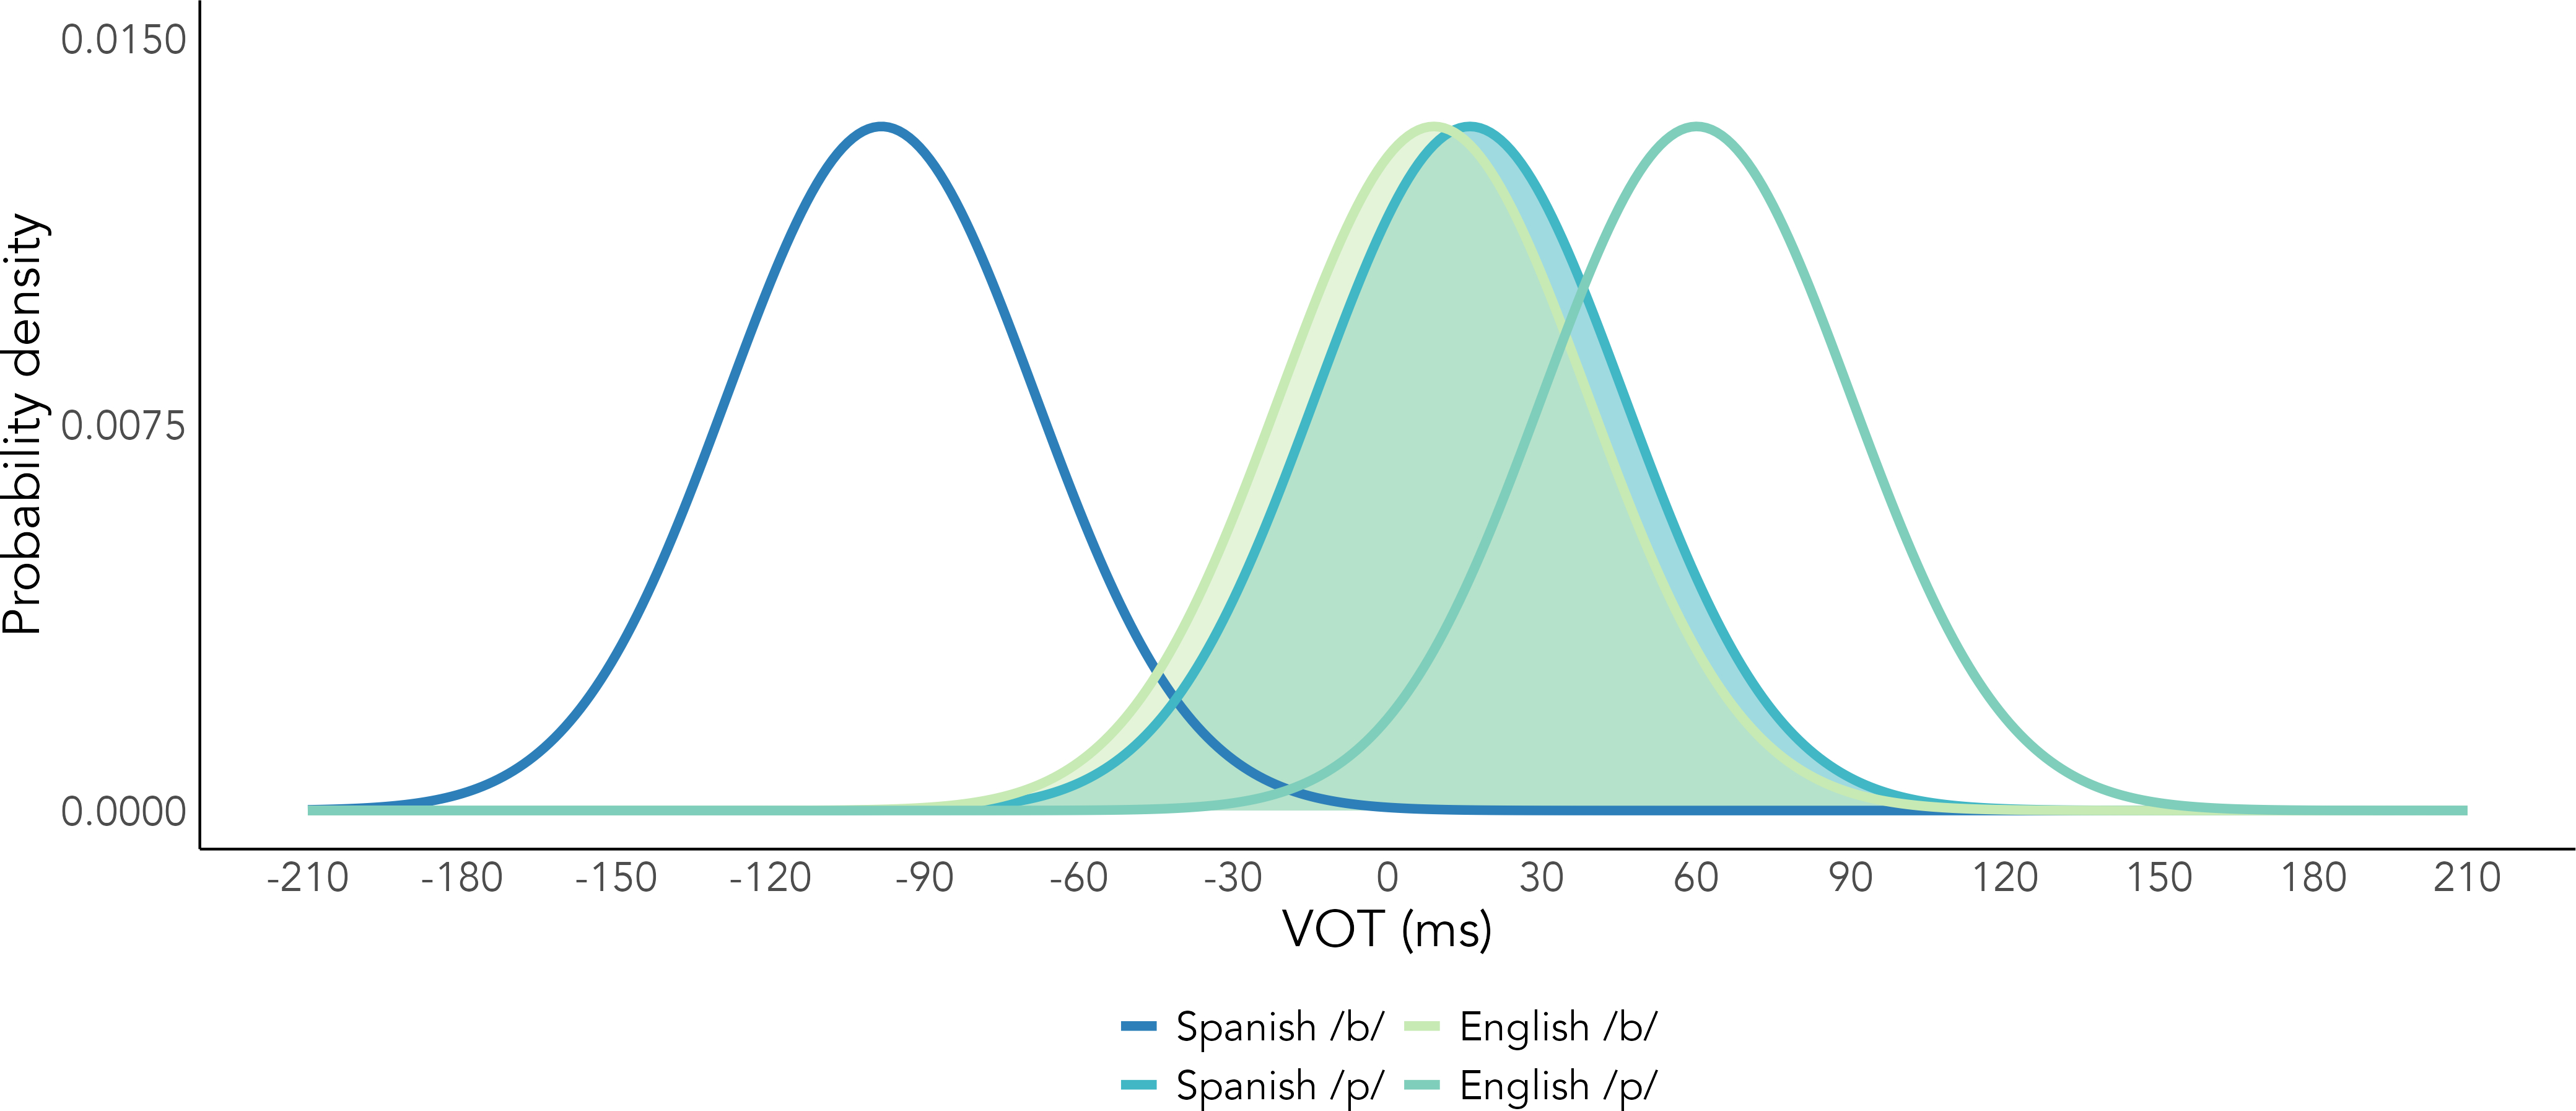
\includegraphics[width=\textwidth]{sections/code/outputs/l1_plot} 

}

\caption{Overlapping VOT distributions for Spanish voiceless stops and English voiced stops.}\label{fig:intro-fig}
\end{figure}

To return to the notion of two-category assimilation, consider an L1 Spanish speaker who is learning English as an L2.
She already has an established /p/-/b/ contrast in her L1 Spanish that is associated with VOT.
The /p/-/b/ contrast in her L2 English is associated with the same cue in the same direction, such that VOTs for /p/ are longer than those for /b/.
As a result, the English /p/-/b/ contrast will be relatively easy to integrate into her existing phonological system compared to, for example, certain vowel contrasts in English (Baigorri et al., 2019).
The same will be true for both the /t/-/d/ and /k/-/g/ contrasts.
However, assimilating the L2 English /p/ to the L1 Spanish /p/ means that the English phoneme will be produced like the Spanish phoneme.
That is, English /p/ will be produced with a short lag VOT (similar to Spanish /p/).
This will create a perceptual problem from a listener's perspective, since short lag VOTs are associated with English /b/, not /p/; without supporting contextual information, listeners may confuse Spanish-accented English /p/ with /b/ (e.g., \emph{park} perceived as \emph{bark}).
To summarize, cross-language transfer in Spanish-accented English can create ambiguity between voiced and voiceless stops (Flege \& Eefting, 1987).
Thankfully, listeners are adept at solving this problem through perceptual adaptation.

\hypertarget{adaptation-in-l1-speech-perception}{%
\subsection{Adaptation in L1 speech perception}\label{adaptation-in-l1-speech-perception}}

Perceptual adaptation is the process of learning the patterns of variation in a speech signal.
Calibrating the perceptual system to novel input allows listeners to map unfamiliar, variable, or secondary acoustic cues onto stable phonetic categories.
Previous research has shown that listeners can use word-level information to guide this learning process.
In a seminal study, Norris et al. (2003) biased listeners toward categorizing ambiguous fricative sounds as /f/ or /s/ by embedding them in different lexical contexts.
For example, the token \emph{proo?} would bias listeners toward categorizing {[}?{]} as /f/ to form the real word \emph{proof} rather than the pseudoword *\emph{proos}.
Listeners who had been exposed to /f/-biased lexical contexts during training were more likely to categorize ambiguous fricative sounds as /f/ rather than as /s/ during test.
This same re-tuning of the perceptual system for specific phonetic contrasts has also been demonstrated in the context of L2-accented speech (Reinisch \& Holt, 2014; Xie et al., 2017; Xie \& Myers, 2017).
Clarke and Luce (2005) exhibited a similar pattern of results with voiceless stops, such that listeners learned to categorize short lag VOTs as /t/ and lead VOTs as /d/ through exposure to supporting lexical contexts.
Importantly, this is the exact shift in VOT that is characteristic of Spanish-accented English stops.
Subsequent studies have also shown that listeners take advantage of VOT and other cues to voicing to adapt to accented speech (Idemaru \& Holt, 2011; Schertz et al., 2016; Wu \& Holt, 2022).
Taken together, these findings suggest that listeners adapt to the shifted VOT-stop mappings in Spanish-accented English through exposure to supporting lexical contexts.

The present dissertation explores two aspects of adaptation to L2-accented speech.
The first aspect of adaptation, investigated in Chapter 2, is how perceptual learning generalizes across talkers.
Previous research has shown that perceptual adaptation to particular cue-category mappings can transfer from one talker to another (Kraljic \& Samuel, 2006, 2007; Reinisch \& Holt, 2014; Xie \& Myers, 2017).
More broadly, the benefits of exposure to an L2 accent can transfer to a new talker with the same accent (e.g., Alexander \& Nygaard, 2019; Sidaras et al., 2009; Tzeng et al., 2016; Xie et al., 2018).
However, there is disagreement in the literature about the conditions under which adaptation generalizes across talkers (Baese-Berk et al., 2013; Bradlow et al., 2023; Bradlow \& Bent, 2008; Xie et al., 2021; Xie \& Myers, 2017).
Study 1, presented in Chapter 2, takes a novel approach to this question using Spanish-accented English VOT-stop mappings as a test case in a series of three behavioral experiments.

The second aspect of adaptation, under investigation in Chapter 3, relates to the neurocognitive correlates underlying perceptual learning.
While there are several theoretical (Goldinger, 1998; Pierrehumbert, 2016; e.g., Sumner et al., 2014) and computational (Kleinschmidt, 2019; Kleinschmidt \& Jaeger, 2015) models of how and why adaptation occurs, the mechanism(s) that support this process are not well-understood (Choi \& Perrachione, 2019; Xie et al., 2023).
One way of investigating these mechanisms is by using time-sensitive neurocognitive methods that can be associated with fine-grained changes in perception.
Study 2, presented in Chapter 3, uses EEG/ERPs to investigate the online linguistic processes associated with adaptation to a Spanish-accented English talker.
Together, these two studies use VOT as a window into perceptual adaptation in brain and behavior.

\newpage

\hypertarget{study-1-the-effects-of-variability-and-similarity-on-generalization-across-spanish-accented-english-talkers}{%
\section{Study 1: The effects of variability and similarity on generalization across Spanish-accented English talkers}\label{study-1-the-effects-of-variability-and-similarity-on-generalization-across-spanish-accented-english-talkers}}

\hypertarget{introduction}{%
\subsection{Introduction}\label{introduction}}

Adaptation to variation in speech is a core aspect of language comprehension.
Without this flexibility, listeners would be unable to make sense of a single talker's vowel space (Whalen et al., 2018), let alone keep track of the innumerable acoustic-phonetic features that vary between talkers (Wade et al., 2007).
This chapter focuses on one facet of adaptation that deals with variation between talkers: generalization.
Here, generalization refers to the ability to apply perceptual learning from one talker or group of talkers to another.
Two aspects of perceptual learning have been shown to facilitate future speech perception: variability during exposure (e.g., Baese-Berk et al., 2013) and similarity between the exposure and test talkers (e.g., Xie \& Myers, 2017).
The present study includes three experiments that directly compare these two factors during exposure to Spanish-accented speech.
The goal is to understand how listeners use acoustic-phonetic information to accommodate variation.

\hypertarget{adaptation-to-l2-accented-speech}{%
\subsubsection{Adaptation to L2-accented speech}\label{adaptation-to-l2-accented-speech}}

Perceptual adaptation research shows that listeners quickly orient to the linguistic features of L2-accented speech (Bent \& Baese-Berk, 2021).
A typical experimental design features an exposure phase, in which participants gain experience with a speech pattern, followed by a test phase.
Talker-specific adaptation is the result of hearing the same talker during exposure and test.
For example, participants who train on Talker A during exposure tend to perform better on Talker A during test than participants who train on Talker B (Bradlow \& Bent, 2008; Clarke \& Garrett, 2004; Xie et al., 2017, 2018, 2021; cf. Bradlow et al., 2023).
Talker-independent adaptation, or generalization, is the result of exposure to a type of talker.
For example, participants who train on Accent X during exposure tend to perform better on Accent X during test than participants who train on Accent Y (Alexander \& Nygaard, 2019; Bradlow \& Bent, 2008; Sidaras et al., 2009; Tzeng et al., 2016; Xie et al., 2018, 2021).
Overall, experience with L2-accented talkers improves perception of novel L2-accented talkers (Baese-Berk et al., 2013; Bieber \& Gordon-Salant, 2022; Reinisch \& Holt, 2014; Tzeng et al., 2024; Witteman et al., 2013).

\hypertarget{talker-independent-adaptation-to-l2-accented-speech}{%
\paragraph{Talker-independent adaptation to L2-accented speech}\label{talker-independent-adaptation-to-l2-accented-speech}}

The pattern of results for talker-independent adaptation becomes more complicated when considering different types of exposure to an accent.
Studies often compare single-talker exposure, in which one talker produces all of the stimuli for a condition, to multi-talker exposure, in which several different talkers produce the stimuli for a condition.
For example, participants in a single-talker exposure condition listen to Talker A with Accent X and participants in a multi-talker exposure condition listen to Talkers B, C, and D with Accent X.
During test, both groups listen to Talker E with Accent X.
Differences in task performance with Talker E index generalization from exposure (Baese-Berk et al., 2013; Bradlow \& Bent, 2008; Xie et al., 2021; Xie \& Myers, 2017).

Experiment 2 of Bradlow and Bent (2008) illustrates how exposure generalizes across L2-accented talkers with the same L1.
In this experiment, participants completed a sentence transcription task during both exposure and test, and performance was measured in terms of sentence recognition accuracy.
There were four key exposure conditions: multi-talker, single-talker, and control.
Participants in the multi-talker condition were exposed to five different Mandarin-accented English talkers, while those in the single-talker condition were exposed to just one Mandarin-accented English talker.
Control training featured five L1-accented English talkers.
Training was followed by two post-tests: one featured a novel talker with a familiar L2 accent (Mandarin) and the other featured a novel talker with an unfamiliar L2 accent (Slovakian).
Performance on the Mandarin-accented English test talker was higher in the multi-talker condition than in the single-talker or control conditions.
By contrast, performance on the Slovakian-accented English test talker did not differ between conditions.
These results suggest that exposure to multiple talkers highlights the characteristic features of an L2 accent.
This experience in turn helps listeners adapt to novel talkers with the same accent.

Baese-Berk et al. (2013) provided evidence that exposure to multiple L2-accented talkers with \emph{different} L1s also facilitates generalization.
They used the same stimulus materials and procedures as Experiment 2 in Bradlow and Bent (2008) in order to compare a multi-accent exposure group directly to the multi-talker exposure and control groups from the previous study.
During multi-accent training, participants were exposed to five L2-accented English talkers, each of whom had a different L1: Thai, Korean, Hindi, Romanian, and Mandarin.
Multi-accent and multi-talker exposure were equally effective at facilitating talker-independent adaptation to the Mandarin-accented test talker relative to control exposure.
Critically, multi-accent exposure also generalized to the Slovakian-accented test talker, while multi-talker and control exposure did not.
Together, these results suggest that exposure to multiple accents highlights the overall features shared by L2 speakers of English.
This experience in turn helps listeners adapt to novel talkers not only with familiar accents, but also with unfamiliar accents.

Xie et al. (2021) investigated the conditions under which single-talker exposure can facilitate generalization.
Specifically, they sought to replicate Bradlow and Bent (2008) with one key change: counterbalancing the test and exposure talkers.
In the original study, different (partially overlapping) sets of Mandarin-accented English talkers were used in the multi-talker and single-talker exposure conditions.
Thus, the lack of generalization from single-talker training may have been the result of the specific talkers, rather than the superiority of multi-talker exposure per se.
The specific combination of exposure and test talkers is likely to have affected performance under both exemplar-based (e.g., Goldinger, 1998; Johnson, 2006), and hybrid (Kleinschmidt \& Jaeger, 2015; e.g., Pierrehumbert, 2016) models of speech perception (see Introduction to Xie et al., 2021).
To address this potential confound, Xie et al. (2021) used a single set of Mandarin-accented talkers for both multi-talker and single-talker exposure; in addition, these talkers were rotated through the exposure talker and test talker roles.
The results replicated Bradlow and Bent (2008)'s finding that multi-talker exposure facilitates generalization more than control exposure.
However, contrary to Bradlow and Bent (2008), they found that single-talker exposure also facilitated generalization more than control exposure.
When comparing multi- and single-talker exposure, the difference in performance depended on the particular combination of exposure and test talkers.
Overall, these results suggest that generalization is strongly influenced by talker-specific features.

Xie and Myers (2017) investigated the acoustic-phonetic features of the exposure talkers that facilitate generalization.
In this study, participants were exposed to Mandarin-accented English through an auditory lexical decision task.
Experimental exposure included multisyllabic real words that biased listeners toward perceiving ambiguous word-final stops as /d/ rather than as /t/ (e.g., \emph{overload}).
Control exposure did not include these critical items.
Both types of exposure featured five Mandarin-accented talkers; the only difference was in the presence of disambiguating lexical contexts for learning ambiguous word-final /d/.
During test, participants performed a primed cross-modal lexical decision task with a novel Mandarin-accented talker.
Previous exposure to Mandarin-accented word-final English /d/ in disambiguating lexical contexts generalized to the novel talker.
Specifically, lexical activation for the /d/-final member of minimal pairs like \emph{seed} versus \emph{seat} was increased in the experimental versus the control group.
The results suggest that listeners did not simply expand their phonetic category boundaries with exposure; instead, they used the lexical contexts from training to re-tune their categories for particular accented features.

Two follow-up experiments with single-talker exposure revealed the importance of exposure-test similarity.
Of the five talkers included in the multi-talker exposure, two were selected.
The first talker was the dissimilar talker, who differed from the test talker on the three key acoustic measures associated with the word-final /t/-/d/ contrast.
The second talker was the similar talker, who did not differ from the test talker in the means of these measures.
Exposure to the similar talker generalized to the test talker, with experimental exposure decreasing lexical competition between \emph{seed}-\emph{seat} minimal pairs compared to control exposure.
By contrast, exposure to the dissimilar talker did not increase performance relative to control exposure.
Moreover, generalization from the similar talker was as strong as generalization from multi-talker exposure (which included this talker).
Together, the results of Xie and Myers (2017) show that the correspondence between exposure and test talkers at the acoustic-phonetic level is critical for understanding the observed patterns of generalization across studies.

\hypertarget{competing-hypotheses-for-generalization}{%
\paragraph{Competing hypotheses for generalization}\label{competing-hypotheses-for-generalization}}

There are two competing explanations for why multi-talker exposure may or may not provide additional benefits for generalization over single-talker exposure: the exposure-to-variability hypothesis and the similarity-based hypothesis.

On the one hand, the exposure-to-variability hypothesis posits that L2-accented talkers exhibit similarities in production that differ from L1-accented norms (Baese-Berk et al., 2013).
The exposure-to-variability hypothesis also posits that among L2-accented talkers with the \emph{same L1}, cross-language influence shifts the relations between acoustic cues and phonetic categories similarly across talkers.
Among L2-accented talkers with \emph{different L1s}, typological features that are unique to the L2 lead to similarly accented realizations regardless of the L1.
Multi-talker exposure thus allows listeners to abstract away from the peculiarities of any given talker and home in on these commonalities.
For example, a listener encountering one unfamiliar Spanish-accented talker may not know whether their short lag VOTs are specific to that talker or characteristic of the L2 accent.
By contrast, a listener encountering multiple unfamiliar Spanish-accented talkers at once would not only see that short lag VOTs are common across the talkers, but also that other accent features (e.g., vowel height) exhibit covariation with voicing (Clayards, 2017).
In Bradlow and Bent (2008), multi-talker exposure outperformed single-talker exposure, suggesting that training on multiple L2-accented talkers (with the same L1) allowed listeners to separate the characteristic features of an accent from the idiosyncratic features of a talker.
The results of Bradlow and Bent (2008) support the exposure-to-variability hypothesis, but do not align with the effects observed by Xie and Myers (2017) and Xie et al. (2021).

On the other hand, the similarity-based hypothesis posits that acoustic-phonetic overlap between the exposure and test talkers, rather than variability during exposure, facilitates generalization (Xie et al., 2021).
In Xie and Myers (2017), listeners exhibited comparable talker-independent adaptation effects after both single- and multi-talker exposure to Mandarin-accented realizations of word-final /d/, which is perceptually confusable with /t/ (e.g., \emph{seed} vs.~\emph{seat}).
Critically, both exposure conditions contained a Mandarin-accented talker with similar word-final /d/ acoustics to the test talker.
Xie et al. (2021) also demonstrated equivalent generalization effects from single- and multi-talker exposure to Mandarin-accented speech.
They argue that exposure to multiple talkers merely increases the likelihood that listeners will encounter a cue distribution that is relevant for adapting to the test talker.
For example, multi-talker training on Spanish-accented speech is more likely to include at least one talker with short lag VOTs than single-talker training.
Bradlow and Bent (2008)'s multi-talker exposure condition may have included talkers who were more similar to the test talker than their single-talker exposure condition, which would confound talker similarity and exposure to variability.
Xie et al. (2021) addressed this confound by counterbalancing the combinations of exposure and test talkers across participants.
Thus, the similarity-based hypothesis may account for the differential effects of single- and multi-talker exposure in perceptual adaptation studies, but further research is needed to distinguish the roles of variability and similarity in talker-independent adaptation.
To summarize, the similarity-based hypothesis focuses on specific cue-category mappings, while the exposure-to-variability hypothesis focuses on the covariation between cues.

\hypertarget{comparing-variability-and-similarity}{%
\subsubsection{Comparing variability and similarity}\label{comparing-variability-and-similarity}}

As discussed above, the results of Bradlow and Bent (2008) support the exposure-to-variability hypothesis, while those of Xie and Myers (2017) and Xie et al. (2021) support the similarity-based hypothesis.
We argue that the socio-indexical structure of cue-category mappings in the ideal adapter framework provides a link between these two hypotheses and can account for these conflicting findings.
According to this theory, listeners represent each cue-category mapping according to informative and useful groupings (Kleinschmidt, 2019).
For L2-accented speech, these groupings may be structured according to each talker (talker-specific) or to the L2 accent shared by the talkers (talker-independent).

The exposure-to-variability hypothesis argues that increasing variability during exposure increases systematic covariation among relevant cues, enabling listeners to separate the idiosyncratic features of a talker from the common features of an accent.
To restate this hypothesis in terms of the ideal adapter framework, covariation among individual exposure talkers promotes the development of a robust talker-independent model (or refinement of an existing one).
In turn, this talker-independent model guides adaptation to the novel test talker.
This exposure-to-variability perspective assumes that talker-independent models are better for generalization than talker-specific models.

By contrast, the similarity-based hypothesis argues that increasing the similarity between the cue-category mappings of the exposure and test talkers facilitates generalization.
Translating this hypothesis into the ideal adapter framework, listeners develop robust talker-specific models during exposure.
During test, listeners use the model that provides the most information about the test talker's cue distributions and most readily predicts their individual cue values to guide adaptation.
This similarity-based perspective assumes that talker-specific models are best for generalization because they provide precise information about cue-category mappings.

Overall, the specificity of a listener's set of generative models may explain the effects of variability and similarity on generalization.
The present study tests these two hypotheses in order to probe the mechanisms underlying adaptation to L2-accented speech.
The overarching goal is to understand how the L1 speech recognition system learns the patterns of cross-language influence in L2 speech production.

\hypertarget{present-study}{%
\subsubsection{Present study}\label{present-study}}

How do listeners generalize their experience with L2-accented speech?
On the one hand, the \emph{structure} of exposure may be the primary driver of talker-independent adaptation.
Variability has been the primary focus of structural inquiries (Baese-Berk et al., 2013), with the number of talkers being the key manipulation (Bieber \& Gordon-Salant, 2022; Bradlow \& Bent, 2008; Choi \& Perrachione, 2019; Xie et al., 2021).
On the other hand, the \emph{content} of exposure may be the key to effective generalization.
At a high level, training on the relevant L2 accent tends to facilitate talker-independent adaptation (Alexander \& Nygaard, 2019; Bradlow et al., 2023; Clarke \& Garrett, 2004; Xie et al., 2018).
At a detailed level, exposure to the relevant acoustic-phonetic features of an L2 accent explains generalization beyond shared L1 (Reinisch \& Holt, 2014; Sidaras et al., 2009; Xie \& Myers, 2017).
Together, a shared L1 and common acoustic-phonetic features create similarity between exposure and test talkers that facilitates adaptation.
The present study builds on this body of work investigating generalization of L2-accented speech.
The key difference between this study and earlier work is the operationalization of variability and similarity.
Specifically, we increased the precision with which variability was implemented (c.f. Baese-Berk et al., 2013) and expanded the scope of similarity (c.f. Xie \& Myers, 2017) in order to better delineate the exposure-to-variability and similarity-based hypotheses.
The goal was to clarify some of the inconsistent findings in the literature for talker-independent adaptation to L2-accented speech (Bent \& Baese-Berk, 2021).

Regarding variability, previous studies have almost exclusively investigated this factor as a comparison between single-talker exposure and multi-talker exposure (c.f. Baese-Berk et al., 2013; Bradlow et al., 2023).
However, multi-talker exposure reduces the amount of experience with any given talker relative to single-talker exposure.
From the larger perceptual adaptation literature, we know that listeners are highly sensitive to acoustic-phonetic mappings and use them to adapt to new talkers (e.g., Kraljic \& Samuel, 2006).
We also know that there is a high degree of within- and between-talker variability in both L1- and L2-accented speech production (Wade et al., 2007; Xie \& Jaeger, 2020).
Depending on the idiosyncrasies of a given exposure talker, altering the amount of experience with this talker may benefit or impede generalization.
This asymmetry in talker-specific exposure may explain some of the inconsistent findings in the literature (Xie et al., 2021; Xie \& Myers, 2017).
Moreover, exposure to multiple talkers increases the sources of covariation to account for, which in turn increases the difficulty of accounting for them during exposure.
If we assume, as the exposure-to-variability hypothesis does, that experience with covariation is critical for generalization, this lack of clarity obscures how and why variability might facilitate generalization.
In the present study, we used a single group of talkers with the same L1 to control the type and amount of experience with each talker across levels of variability.

Regarding similarity, previous studies have either conceptualized this factor at the accent level or at the acoustic-phonetic level.
When it comes to operationalizing either definition of similarity, we run into the same problem as we did with multi-talker versus single-talker exposure.
That is, we end up comparing two (or more) groups of exposure talkers between conditions.
If we assume again that listeners are highly sensitive to talker-specific acoustic-phonetic features, then this design confounds talker- and accent-specific effects.
In other words, we cannot know whether listeners are ``learning a talker or learning an accent'' or learning both (Xie \& Myers, 2017).
Here, we manipulated the stimuli listeners encounter during exposure rather than the talkers in order to maintain consistency across levels of similarity.
Moreover, we directly crossed the factors of similarity and variability in the same design, which, to our knowledge, has not yet been done.
Overall, this study allows us to address the ongoing debate between the exposure-to-variability and similarity-based hypotheses for generalization.

\hypertarget{norming-study}{%
\subsection{Norming study}\label{norming-study}}

\hypertarget{methods-pars-norm}{%
\subsubsection{Participants}\label{methods-pars-norm}}

Prior to conducting the main experiments, we recruited a separate group of participants (\emph{N} = 688) from the Penn State subject pool to norm the auditory stimuli.
Participants provided implied consent in line with Penn State IRB policies and were compensated 0.5 class credits after completing the experiment, which took 15-30 minutes.
Eligible participants were between the ages of 18 and 40 years, spoke English as their first and only fluent language, had normal hearing, had normal or corrected-to-normal vision, and did not have a history of language-related disorders.
We removed ineligible participants (\emph{N} = 34) and those with poor data quality (\emph{N} = 83; see Section \ref{methods-analysis-norm}) from further analysis.
This left 571 participants.

\hypertarget{methods-stims}{%
\subsubsection{Stimuli}\label{methods-stims}}

Stimuli were grouped by onset phoneme (e.g., \emph{park} has the onset phoneme /p/).
There were three \textbf{experimental onset} groups: critical, competitor, and control.
Critical onsets were voiceless stops (/p/, /t/, and /k/), competitor onsets were voiced stops (/b/, /d/, and /g/), and control onsets were voiceless fricatives (/f/, /s/, and /\textipa{S}/).
Across the experimental onset groups, phonemes were also grouped (roughly) according to their place of articulation: labial (/p/, /b/, and /f/), alveolar (/t/, /d/, and /s/), and postalveolar/velar (/k/, /g/, and /\textipa{S}/).
These will be referred to as the \textbf{cross-experimental onset} groups.
There was one \textbf{filler onset} group: /m/, /n/, /l/, /\textipa{\*r}/, /h/, and /w/.
Filler onsets were also grouped by their place of articulation: nasal (/m/ or /n/), alveolar (/l/ or /\textipa{\*r}/), and other back consonants (/h/ or /w/).
These will be referred to as the \textbf{within-filler onset} groups.
Finally, each cross-experimental onset group was paired with one of the within-filler onset groups according to frontness/backness: front (/p/, /b/, /f/, /m/, and /n/), mid (/t/, /d/, /s/, /l/, and /\textipa{\*r}/), and back (/k/, /g/, /\textipa{S}/, /h/, and /w/).
These will be referred to as the \textbf{cross-condition onset} groups.

Stimulus selection began by downloading real words with one to four syllables, three to eight letters, and one to two morphemes from the English Lexicon Project (ELP) restricted lexicon (Balota et al., 2007).
Within this set of items, we limited our search to words with experimental or filler onsets followed directly by a vowel (e.g., \emph{peach} was considered but \emph{preach} was not).
We removed duplicate word stems with different suffixes (e.g., \emph{paints} and \emph{painting} were removed but \emph{paint} was kept).
We also removed any inappropriate, harmful, or distracting words and word stems.
The remaining set of items will be referred to as the ELP pool.

Multisyllabic stimulus selection began by drawing real words with two to four syllables, five to eight letters, and one to two morphemes from the ELP pool.
We removed words with minimal pairs between the critical and competitor groups (e.g., \emph{pocket} and \emph{docket} were removed but \emph{socket} and \emph{locket} were kept).
Once the set of options was established, real words were selected and pseudowords were created.
Pseudowords were created by changing the onsets of real words with filler onsets that had not been selected as potential real words for the study.
For experimental pseudowords, onsets were assigned according to the cross-condition onset groups (e.g., \emph{machine} became *\emph{pachine}, *\emph{bachine}, and *\emph{fachine}).
For filler pseudowords, one of the other five filler onsets was substituted for the existing filler onset (e.g., \emph{medicine} became *\emph{hedicine}).
In total, 544 multisyllabic real words and 555 multisyllabic pseudowords were normed.

Monosyllabic stimulus selection began by drawing real words with one syllable, three to six letters, and one morpheme from the ELP pool.
From this set of options, we pulled all words with critical onsets that had cross-experimental minimal pairs with competitor onsets (e.g., \emph{park}-\emph{bark}).
Both members of each critical-competitor minimal pair were normed.
We also selected words with filler onsets that had a minimal pair with a different filler onset (e.g., \emph{mall}-\emph{hall}).
In total, 319 monosyllabic real words were normed.

Norming took place in three waves of testing.
Overall, there were nine experimental lists of 180 to 540 items: three in the first wave, two in the second, and four in the third.
Lists always contained an equal number of real words and pseudowords, and items from each experimental onset groups were always presented in separate lists.

\hypertarget{methods-rec}{%
\subsubsection{Recording}\label{methods-rec}}

One female L1-accented English talker from the US (Talker 0; the first author) recorded all of the items.
Audio was captured with a head-worn condenser microphone (Shure SM35-XLR) connected to an audio interface (Sound Devices USBPre2) and recorded with Praat (Broersma \& Weenink, 2021) in mono at 44.1 kHz in a sound-attenuated booth.
After annotating the recordings and extracting the individual sound files, stimuli were normalized to 70 dB and had 50 ms of silence added to the beginning and end.

\hypertarget{task-and-procedure}{%
\subsubsection{Task and procedure}\label{task-and-procedure}}

The study was conducted online using Pavlovia.
At the beginning of the study, participants responded to a yes/no question for each eligibility criterion.
Ineligible participants were not able to complete the study.

The study featured an auditory lexical decision task.
Participants were randomly assigned to an experimental list.
On each trial, participants indicated whether an auditory stimulus was a real English word or not by pressing the \emph{d} or \emph{k} key on their keyboard.
One of the two response-key relations---real-\emph{d} or real-\emph{k}---was assigned randomly to each participant.
The total number of trials varied by list.

\hypertarget{methods-analysis-norm}{%
\subsubsection{Analysis}\label{methods-analysis-norm}}

Analyses were conducted with R version 4.2.2 using the \emph{stats} package (R Core Team, 2022).
Each wave of testing was analyzed separately.
The experimental lists within each wave were combined for analysis.
We first conducted t-tests comparing each participant's accuracy to chance (50\%) to check for data quality.
Data from participants whose performance was indistinguishable from chance were removed from further analysis (see Section \ref{methods-pars-norm}).
Next, we conducted t-tests comparing the accuracy on each item to chance (50\%).
Items that did not yield above-chance accuracy were removed from further consideration.
All three variants of each experimental pseudoword and both members of each cross-experimental minimal pair needed to have above-chance accuracy in order to be considered for final selection.
The set of items that passed the norming phase will be referred to as the selection pool.
For details on the stimuli that were selected for Experiment 1, see Section \ref{methods-lists-1a}.

\hypertarget{experiment-1-investigating-differences-in-generalization-from-exposure-to-spanish-accented-stops-versus-fricatives}{%
\subsection{Experiment 1: Investigating differences in generalization from exposure to Spanish-accented stops versus fricatives}\label{experiment-1-investigating-differences-in-generalization-from-exposure-to-spanish-accented-stops-versus-fricatives}}

\hypertarget{methods}{%
\subsubsection{Methods}\label{methods}}

We used an exposure-test design to understand how different kinds of experience with Spanish-accented speech change listeners' VOT-stop mappings.
The exposure phase established the comparison between the similarity-based and exposure-to-variability hypotheses of talker-independent adaptation.
The test phase assessed the effects of each type of exposure on perception.

\hypertarget{methods-design-1a}{%
\paragraph{Design}\label{methods-design-1a}}

Participants were exposed to multisyllabic real words and pseudowords before being tested on monosyllabic real words.
Participants heard these items produced by four Spanish-accented talkers: three during exposure and one during test.
During exposure, multisyllabic items without onset competitors provided disambiguating lexical contexts for categorizing Spanish-accented onsets.
For example, consider the real word \emph{pencil} and the pseudoword *\emph{pachine}.
In both cases, the onset may be interpreted as /p/ or /b/.
This ambiguity does not affect whether *\emph{pachine} is perceived as a real word or not, since both *\emph{pachine} and *\emph{bachine} are pseudowords.
However, resolving this ambiguity is necessary for distinguishing between the real word \emph{pencil} and pseudoword *\emph{bencil}.
Critically, participants hearing ambiguous real words like \emph{pencil} would never hear unambiguous real words like \emph{beehive}.
Thus, in the context of the exposure task, participants should learn to perceive the ambiguous short lag VOTs as /p/ rather than as /b/.
During test, monosyllabic items with onset competitors created ambiguous lexical contexts in which to assess learning from exposure.

\textbf{Exposure similarity} was operationalized as the relation between the experimental onsets encountered during exposure and the critical onsets encountered during test.
There were three levels of Similarity: Direct, Indirect, and Control.
Each level refers to the type of information participants received about Spanish-accented voiceless stops.
In Direct conditions, participants were exposed directly to critical onsets (e.g., \emph{pencil} and *\emph{pachine}).
In Indirect conditions, participants were exposed to competitor onsets (e.g., \emph{beehive} and *\emph{bachine}), thereby gaining experience with the shifted VOT continuum that they would encounter during test.
In Control conditions, participants were exposed to control onsets (e.g., \emph{football} and *\emph{fachine}), thereby gaining general experience with Spanish-accented speech but not with stop VOTs.
This design allowed the talkers to remain the same across the three levels of Similarity.

\textbf{Exposure variability} was operationalized as the relation between onset phonemes and exposure talkers.
There were two levels of Variability: Invariant and Variant.
Each level refers to the type of experience with each talker.
This is illustrated in Figure \ref{fig:exp1-fig}.
In Invariant conditions, listeners heard each of the three exposure talkers produce one onset out of the three in an experimental group (e.g., Direct-Invariant: Talker A produced \emph{pencil}, Talker B produced \emph{tablet}, and Talker C produced \emph{kingdom}).
This means that all of the words with a given onset were produced by one talker.
In Variant conditions, listeners heard each of the three exposure talkers produce all three onsets in an experimental group (e.g., Direct-Variant: Talker A produced \emph{pencil}, \emph{tablet}, and \emph{kingdom}).
This means that one third of the words with a given onset were produced by each talker.
This design allowed the items and talkers to remain the same between levels of Variability.

The two exposure factors of Similarity (Direct, Indirect, Unrelated) and Variability (Variant, Invariant) were manipulated between participants, so each participant was assigned to one of the six combinations of Similarity and Variability.
Target type was manipulated within participants.
There were three levels of Target: Identity, Competitor, and Unrelated (See Figure \ref{fig:exp1-fig}).
Each level refers to the type of visual target that followed each auditory prime.
Identity targets exactly matched the auditory primes (e.g., \emph{park}-\emph{park}).
Competitor targets were the minimal pairs of the auditory primes (e.g., \emph{park}-\emph{bark}).
Unrelated targets only shared vowels with the auditory primes (e.g., \emph{park}-\emph{wand}).
Differential performance on these three conditions indexed learning from exposure.

\begin{figure}[H]

{\centering 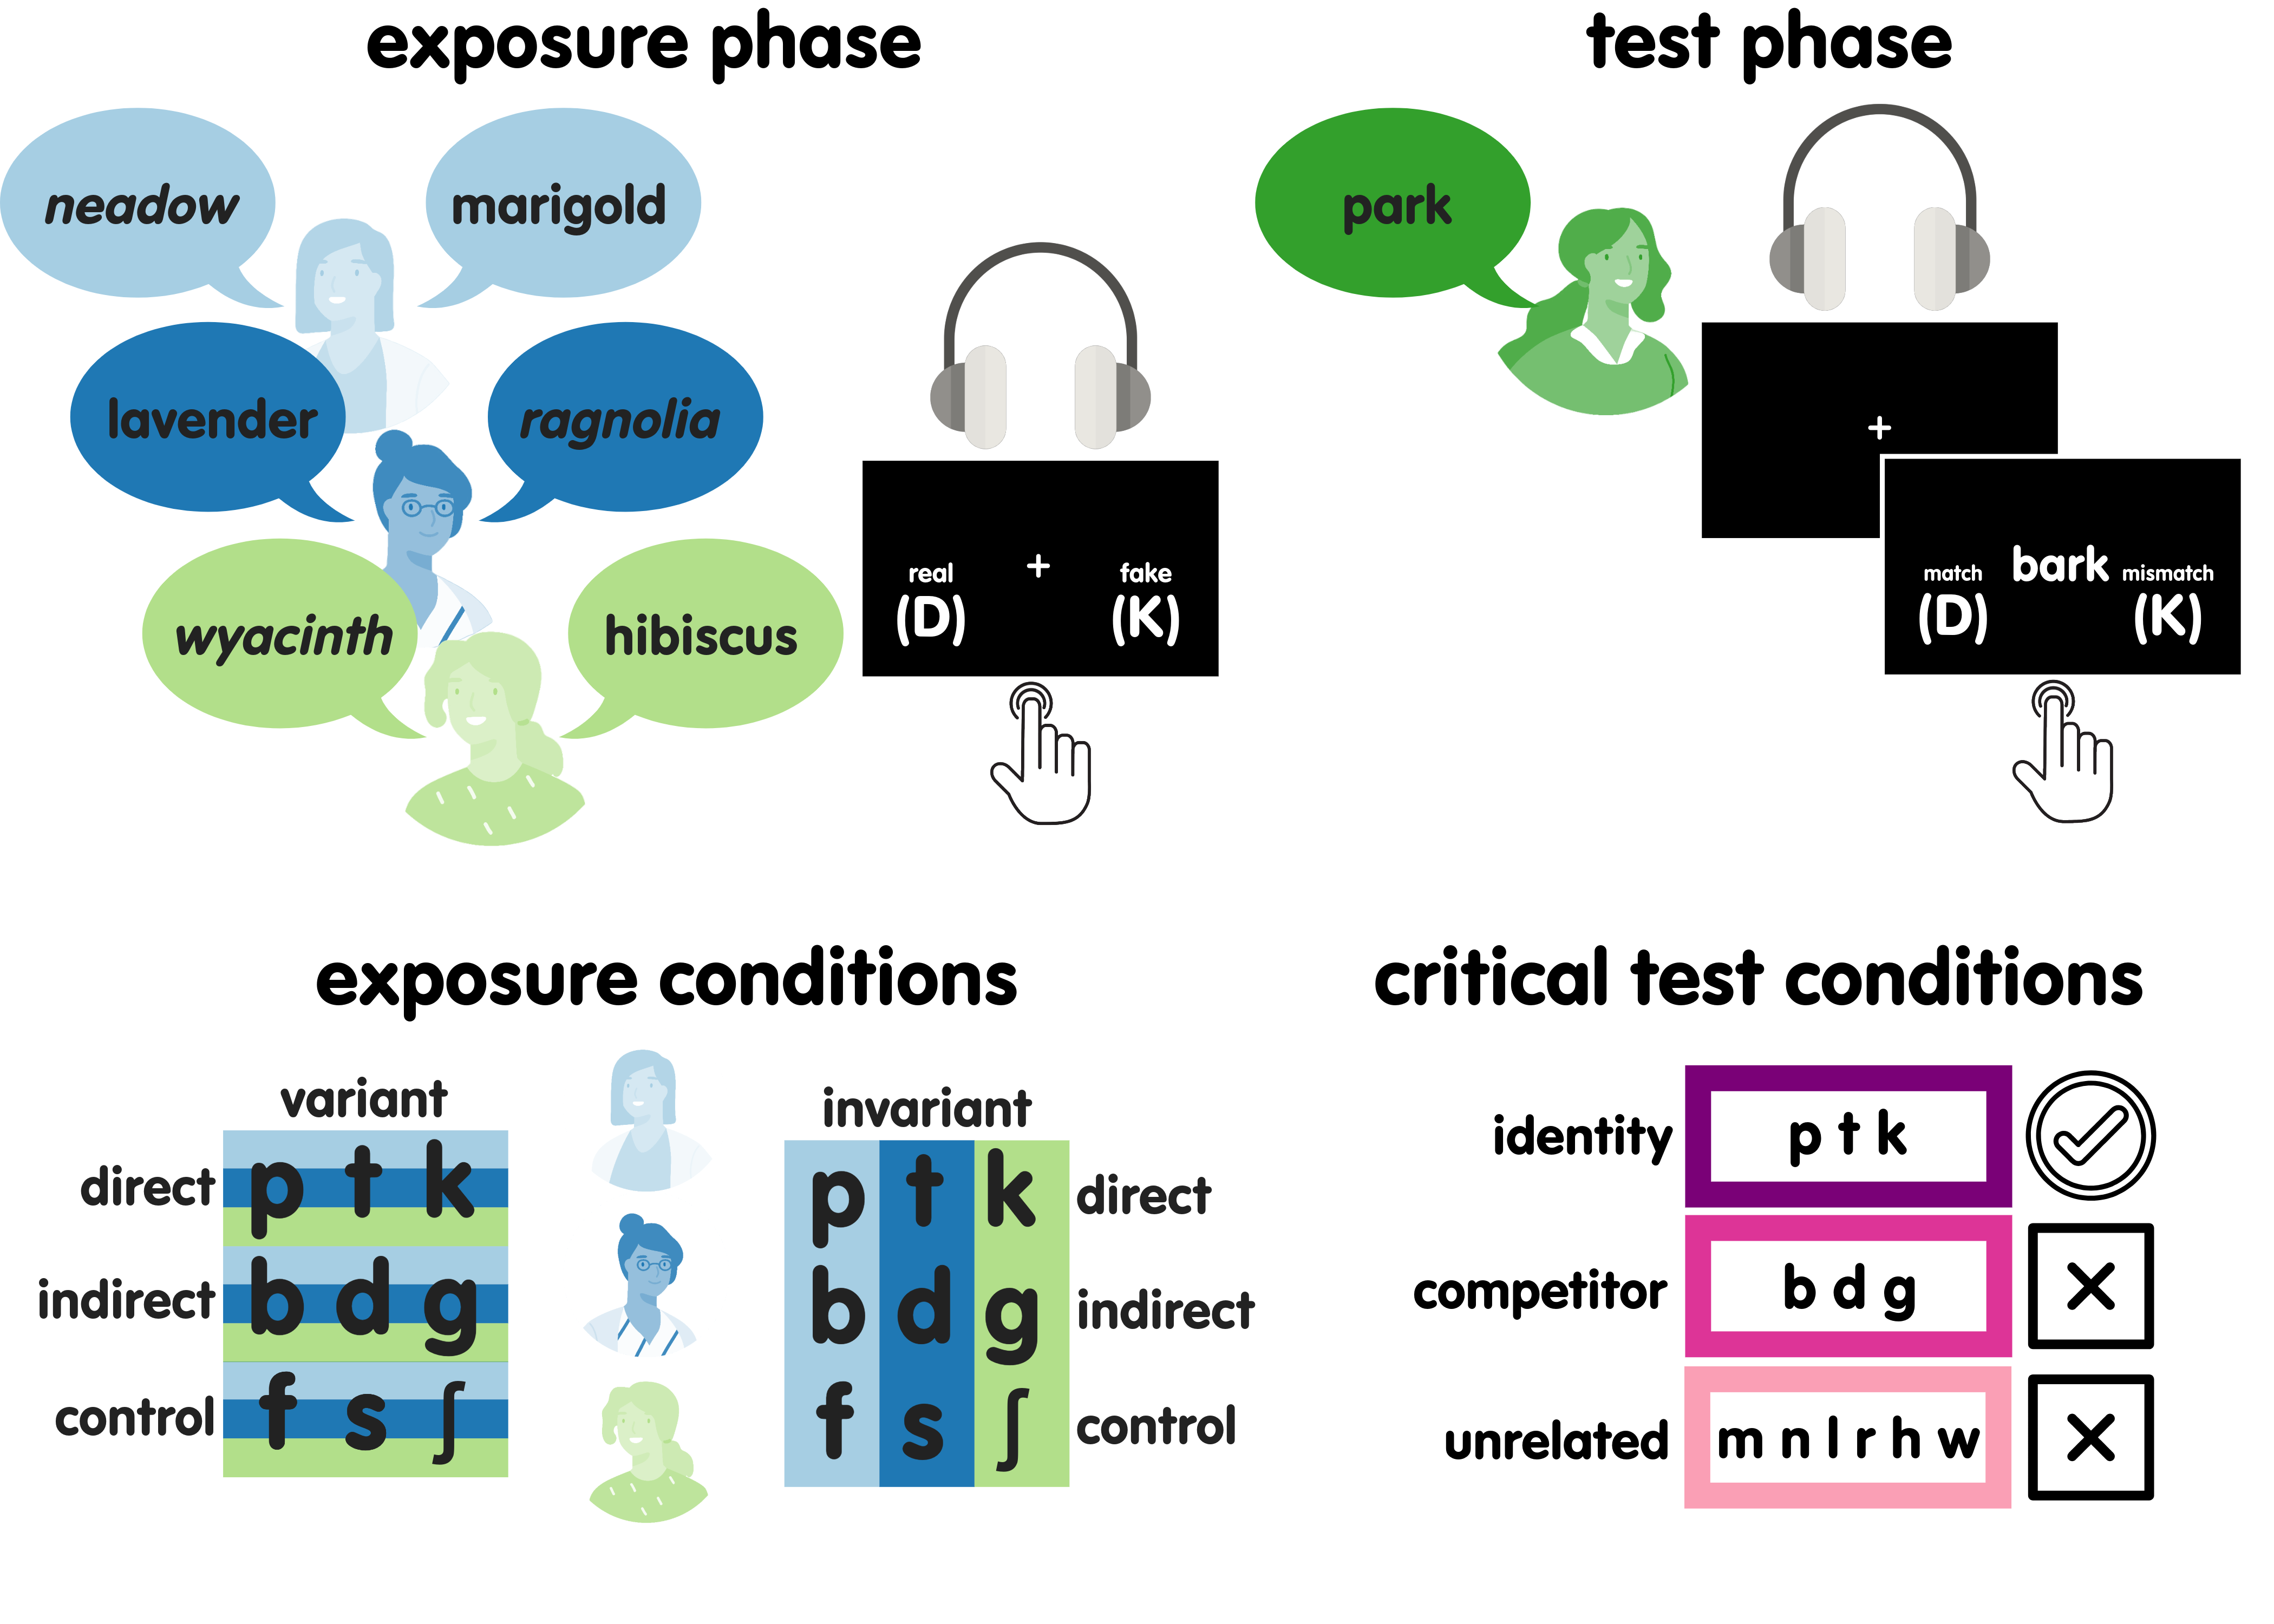
\includegraphics[width=\textwidth]{figures/diss_1} 

}

\caption{Experiment 1 design.}\label{fig:exp1-fig}
\end{figure}

\hypertarget{methods-pars-1a}{%
\paragraph{Participants}\label{methods-pars-1a}}

We recruited 296 participants through the online platform Prolific.
Participants provided implied consent in line with Penn State IRB policies and were compensated \$6 after completing the experiment, which took approximately 30 minutes.
The experiment was available to individuals whose Prolific user profiles aligned with the following eligibility criteria: between 18 and 40 years of age, located in the US at the time of the study, English as their first and only fluent language, normal hearing, normal or corrected-to-normal vision, and without a history of language-related disorders.
The Prolific user profiles for each participant also included sex (two options, select one) and race/ethnicity information (four options, select all that apply).

The eligibility criteria were cross-checked with the responses to a post-experiment questionnaire (see Section \ref{methods-tasks-1a}), and any ineligible participants was removed from further analysis (\emph{N} = 9).
We also removed participants with any knowledge of Spanish, with self-rated proficiency greater than or equal to 3/5 in any languages other than English, with self-rated proficiency less than 5/5 in English, or whose place of origin was not the US (\emph{N} = 15).
This left 287 eligible participants.

Finally, we removed participants with poor data quality from further analysis (\emph{N} = 15).
Poor data quality was defined as: accuracy statistically indistinguishable from or significantly below chance on experimental real words in the exposure task, zero correct experimental trials in any of the three conditions in the test task, or fewer than 50\% of experimental trials with correct responses and reaction times between 50 and 2500 ms in either task (see Section \ref{methods-tasks-1a} for details).
These criteria were chosen to balance the level of performance with the amount of data available for analysis.
This left 257 participants for analysis (Age: \emph{M} = 31, \emph{SD} = 6, Min = 18, Max = 40; Sex: Female = 121, Male = 135, Prefer not to say = 1; Race: Asian = 5, Black = 43, Multiple selected = 21, Other = 5, White = 182, Not provided = 1).

We recruited 46 additional participants through Prolific to complete the experiment without the exposure phase.
Removing ineligible participants left 38 participants.
Removing participants with low data quality left 37 participants for analysis (Age: \emph{M} = 31, \emph{SD} = 5, Min = 21, Max = 40; Sex: Female = 19, Male = 18; Race: Asian = 2, Multiple selected = 5, Other = 2, White = 28).
All aspects of recruitment were the same for this group as for the main group of participants.

\hypertarget{methods-talk-1a}{%
\paragraph{Talkers}\label{methods-talk-1a}}

Seven female Spanish-accented English talkers from Latin America and Spain were recruited to be talkers for the experiment.
Talkers were compensated with one \$20 Amazon giftcard per recording session (30-60 minutes each; 1-2 total).
Recording followed the procedure described in Section \ref{methods-rec}.

Out of the seven talkers, we selected four from Mexico (Talkers 1-4) to control for country-level dialectal variation in the L1.
Each talker was from a different region of Mexico and reported living in this region for the majority of their lives before moving to the US for college or graduate school.
All four talkers reported that they grew up speaking Spanish with their caregivers and began acquiring English in traditional classroom settings.
Language background information for each talker is provided in Table \ref{tab:spk-tab}.

\begin{table}

\caption{\label{tab:spk-tab}Talker background information.}
\centering
\resizebox{\linewidth}{!}{
\begin{tabular}[t]{r|l|r|r|r}
\hline
Talker & Region & Age of English acquisition & Age of arrival in US & Age at time of recording\\
\hline
1 & Veracruz, Mexico & 10 & 18 & 26\\
\hline
2 & Quintana Roo, Mexico & 13 & 26 & 28\\
\hline
3 & Puebla, Mexico & 5 & 24 & 27\\
\hline
4 & Mexico City, Mexico & 5 & 28 & 31\\
\hline
\end{tabular}}
\end{table}

\hypertarget{methods-stims-1a}{%
\paragraph{Stimuli}\label{methods-stims-1a}}

In total, there were 936 auditory items and 648 visual items across tasks.
The exposure task featured multisyllabic real words and pseudowords with experimental and filler onsets from the selection pool.
The final set of exposure items included 360 real words (24 per onset) and 360 pseudowords (24 per onset).
The test task featured two types of stimuli: auditory primes and visual targets.
Auditory primes were monosyllabic real words with critical or filler onsets from the selection pool.
The final set of auditory primes included 216 real words (24 per onset).
The final set of visual targets included 648 real words (3 per prime; see below for details).

During auditory stimulus selection, we considered a number of parameters.
From the ELP, we included word length, orthographic neighborhood density (OND), phonological neighborhood density (PND), and US Zipf frequency.
From Brysbaert et al. (2019), we included percent known and prevalence.
We also included the position of lexical stress, calculated from the pronunciation information provided by the ELP, and mean lexical decision accuracy from norming (LDT).
The final set of exposure real words was chosen such that the four groups of stimuli---Direct, Indirect, Control, and Filler---were equivalent on each of these parameters.
We conducted t-tests comparing each group on each parameter to ensure that they were not significantly different (\emph{ps} \textgreater{} .05).
The final set of auditory primes for the test task was selected in a similar way.
We conducted t-tests comparing the Critical and Filler primes on every parameter except for lexical stress, which was not relevant for monosyllabic words (\emph{ps} \textgreater{} .05).
We also conducted pairwise t-tests between Critical primes and their Competitor pairs (\emph{ps} \textgreater{} .05).
The final set of exposure pseudowords was chosen such that the four groups of stimuli were equivalent in length, position of lexical stress, and mean lexical decision accuracy.
The other parameters were either not available (OND and PND) or not relevant (US Zipf frequency, percent known, prevalence) for the pseudowords.
The relevant parameters for each group of stimuli are shown in Table \ref{tab:stim-tab}
Descriptive statistics for each talker's real word VOTs by onset are provided in Table \ref{tab:spk-vot-tab}.

\begin{table}

\caption{\label{tab:stim-tab}Mean and standard deviation of stimulus parameters by condition and task.}
\centering
\resizebox{\linewidth}{!}{
\begin{tabular}[t]{l|l|l|r|l|l|l|l|l|l|l|l}
\hline
Phase & Word type & Condition & N & Length & LDT & Lexical stress & OND & PND & Frequency & Percent known & Prevalence\\
\hline
 &  & Direct & 72 & 6.85 (0.93) & 0.89 (0.09) & 1.11 (0.32) & 0.56 (1.40) & 1.12 (2.13) & 3.38 (0.74) & 0.98 (0.02) & 2.12 (0.29)\\
\cline{3-12}
 &  & Indirect & 72 & 6.82 (0.98) & 0.89 (0.08) & 1.21 (0.41) & 0.62 (1.34) & 1.14 (2.04) & 3.45 (0.72) & 0.99 (0.02) & 2.16 (0.29)\\
\cline{3-12}
 &  & Control & 72 & 6.93 (0.95) & 0.87 (0.09) & 1.15 (0.36) & 0.67 (1.17) & 1.76 (2.76) & 3.39 (0.77) & 0.98 (0.03) & 2.11 (0.38)\\
\cline{3-12}
 & \multirow{-4}{*}{\raggedright\arraybackslash Real word} & Filler & 144 & 6.83 (0.95) & 0.87 (0.10) & 1.12 (0.32) & 0.78 (1.52) & 1.49 (2.66) & 3.42 (0.77) & 0.98 (0.03) & 2.14 (0.35)\\
\cline{2-12}
 &  & Direct & 72 & 7.08 (0.87) & 0.89 (0.06) & 1.22 (0.42) &  &  &  &  & \\
\cline{3-12}
 &  & Indirect & 72 & 7.08 (0.87) & 0.88 (0.07) & 1.22 (0.42) &  &  &  &  & \\
\cline{3-12}
 &  & Control & 72 & 7.08 (0.87) & 0.88 (0.06) & 1.22 (0.42) &  &  &  &  & \\
\cline{3-12}
\multirow{-8}{*}{\raggedright\arraybackslash Exposure} & \multirow{-4}{*}{\raggedright\arraybackslash Pseudoword} & Filler & 144 & 6.93 (1.01) & 0.88 (0.05) & 1.14 (0.35) &  &  &  &  & \\
\cline{1-12}
 &  & Critical prime & 72 & 3.88 (0.63) & 0.88 (0.07) &  & 11.36 (5.21) & 21.85 (7.96) & 4.15 (0.94) & 0.99 (0.04) & 2.22 (0.34)\\
\cline{3-12}
 &  & Competitor pair & 72 & 3.90 (0.65) & 0.88 (0.08) &  & 10.39 (5.02) & 21.15 (7.12) & 4.09 (1.11) & 0.98 (0.05) & 2.10 (0.42)\\
\cline{3-12}
\multirow{-3}{*}{\raggedright\arraybackslash Test} & \multirow{-3}{*}{\raggedright\arraybackslash Real word} & Filler prime & 144 & 3.90 (0.58) & 0.90 (0.08) &  & 10.49 (4.70) & 22.27 (8.89) & 4.15 (0.97) & 0.99 (0.02) & 2.22 (0.32)\\
\hline
\multicolumn{12}{l}{\rule{0pt}{1em}Competitor pairs were presented as visual targets only}\\
\end{tabular}}
\end{table}

\begin{table}

\caption{\label{tab:spk-vot-tab}Mean, standard deviation, and range of VOTs by onset by talker.}
\centering
\resizebox{\linewidth}{!}{
\begin{tabular}[t]{l|l|r|r|r|l|r|r|l|r|r|l|r|r|l}
\hline
\multicolumn{3}{c|}{ } & \multicolumn{3}{c|}{Talker 1} & \multicolumn{3}{c|}{Talker 2} & \multicolumn{3}{c|}{Talker 3} & \multicolumn{3}{c}{Talker 4} \\
\cline{4-6} \cline{7-9} \cline{10-12} \cline{13-15}
Phase & Onset & \textit{N} & \textit{M} & \textit{SD} & Range & \textit{M} & \textit{SD} & Range & \textit{M} & \textit{SD} & Range & \textit{M} & \textit{SD} & Range\\
\hline
 & /b/ & 24 & -21 & 51 & -132-48 & 15 & 27 & -87-77 & -44 & 52 & -150-31 & -69 & 53 & -133-103\\
\cline{2-15}
 & /p/ & 24 & 73 & 26 & 24-122 & 61 & 41 & 11-160 & 82 & 26 & 37-123 & 21 & 17 & 6-69\\
\cline{2-15}
 & /d/ & 24 & 2 & 42 & -100-39 & 21 & 22 & -75-53 & 8 & 29 & -54-33 & -78 & 53 & -177-44\\
\cline{2-15}
 & /t/ & 24 & 72 & 20 & 36-112 & 65 & 22 & 25-109 & 91 & 28 & 46-157 & 41 & 15 & 18-74\\
\cline{2-15}
 & /g/ & 24 & 2 & 55 & -104-68 & 31 & 25 & -75-51 & -5 & 51 & -148-47 & -64 & 65 & -229-67\\
\cline{2-15}
\multirow{-6}{*}{\raggedright\arraybackslash Exposure} & /k/ & 24 & 82 & 28 & 33-151 & 88 & 21 & 49-123 & 96 & 23 & 43-133 & 48 & 16 & 25-77\\
\cline{1-15}
 & /p/ & 24 & 71 & 28 & 19-126 & 60 & 35 & 10-118 & 115 & 39 & 15-201 & 26 & 24 & 8-106\\
\cline{2-15}
 & /t/ & 24 & 78 & 21 & 27-109 & 61 & 20 & 28-106 & 102 & 23 & 60-142 & 53 & 27 & 8-99\\
\cline{2-15}
\multirow{-3}{*}{\raggedright\arraybackslash Test} & /k/ & 24 & 94 & 21 & 70-171 & 94 & 20 & 50-133 & 119 & 40 & 65-244 & 65 & 30 & 21-124\\
\hline
\end{tabular}}
\end{table}

An additional set of six real words and six pseudowords with filler onsets (one per onset per word type) was selected for practice.
Six additional primes with filler onsets (one per onset) were also selected for practice.

Visual targets in the test task were monosyllabic real words with critical, competitor, or filler onsets.
Each auditory prime had three visual targets: one was the prime itself, one was its minimal pair, and one was unrelated.
The first two were determined by the prime, but the third needed to be selected separately.
Each unrelated target had a filler onset and was chosen to have the same vowel as the prime but a different onset and offset.
These items were primarily from the selection pool, but some were from the larger ELP pool.
Two additional unrelated targets were also selected for practice.

\hypertarget{methods-lists-1a}{%
\paragraph{Experimental lists}\label{methods-lists-1a}}

Combining Similarity and Variability created six between-subjects conditions: Direct-Variant, Direct-Invariant, Indirect-Variant, Indirect-Invariant, Control-Variant, and Control-Invariant.
In addition, one group of participants did not receive any exposure prior to test; this will be referred to as the Test-only condition.
The 288 filler items were the same across conditions and evenly divided by word type---real word and pseudoword---as well as by onset---/m/, /n/, /l/, /\textipa{\*r}/, /h/, and /w/.
The 144 experimental items were evenly divided by onset and word type, with onset differing by level of Similarity: Direct (critical: /p/, /t/, and /k/), Indirect (competitor: /b/, d/, and /g/), and Control (control: /f/, /s/, and /\textipa{S}/).
As a result, there were 24 items per onset per word type.

The assignment of talkers to items differed by level of Variability.
In Invariant conditions, talkers were assigned by cross-condition onset group: front (/p/, /b/, /f/, /m/, and /n/), mid (/t/, /d/, /s/, /l/, and /\textipa{\*r}/), and back/other (/k/, /g/, /\textipa{S}/, /h/, and /w/).
In other words, one talker was assigned to front onsets, one to mid, and one to back/other.
Within a given level of Similarity, this means that each talker produced items with one out of the three experimental onsets and two out of the six filler onsets.
For Variant conditions, one third of each of the items of a given onset and word type (8) was randomly assigned to one of three sets: set 1, set 2, or set 3.
Each set was assigned to one talker.

To counterbalance which talkers were assigned to which items across participants, each Variant item set was paired with one Invariant onset group to create three assignment groups: group 1 (front with set 1), group 2 (mid with set 2), and group 3 (back/other with set 3).
In addition, we also counterbalanced the talkers between the exposure and test phases.
To do this, we added group 4 (test) and rotated the four talkers across these four assignment groups in a Latin square design.
Overall, this resulted in 24 experimental lists for the exposure phase, one for each combination of exposure condition (6) and talker assignment (4).

Regardless of exposure condition, all participants heard the same 216 auditory primes during test.
One third (72) were critical items divided evenly by onset---/p/, /t/, and /k/---and two thirds (144) were filler items divided evenly by onset---/m/, /n/, /l/, /\textipa{\*r}/, /h/, and /w/.
Each onset was divided evenly by target type---Identity, Competitor, and Unrelated.
This resulted in eight items per onset per target type
Three experimental lists were created to counterbalance the combinations of auditory prime and visual target across participants.
Since the test talker was also counterbalanced across participants, this resulted in 12 experimental lists for the test phase, one for each combination of prime-target pair (3) and talker assignment (4).

Exposure practice was presented in Talker 0's voice for all participants.
Test practice was presented according to the participant's talker assignment and Variability condition.
Participants in the Test-only condition completed the test practice in Talker 0's voice.

\hypertarget{methods-tasks-1a}{%
\paragraph{Tasks}\label{methods-tasks-1a}}

The experiment included a headphone check, exposure task, test task, and post-experiment questionnaire.
All aspects of the experiment were conducted online using Pavlovia.
The headphone check, exposure task, and test task were created in PsychoPy Builder (Peirce et al., 2019).
The post-experiment questionnaire was built using Pavlovia's survey platform.

The headphone check followed the anti-phase tone test procedure from Woods et al. (2017).
On each trial, participants listened to three pure tones, one of which was out of phase with the other two.
Participants indicated which of the three tones was the quietest by selecting the appropriate button on the screen: tone 1, tone 2, or tone 3.
There were two trials per response for a total of six trials, which were presented in random order.
Participants using well-functioning headphones should have easily perceived the anti-phase tone as the quietest, while those using loudspeakers should not.
Participants completed the task at most two times.

The exposure phase featured the auditory lexical decision task from Xie and Myers (2017).
On each trial, participants indicated whether an auditory stimulus was a real English word or not by pressing the \emph{d} or \emph{k} key on their keyboard.
One of the two response-key relations---real-\emph{d} or real-\emph{k}---was assigned randomly to each participant.
Participants completed 12 practice trials followed by 432 main trials presented in random order.
Half of the practice trials (6) and half of the main trials (216) required real word responses.

The test phase featured a cross-modal matching task adapted from the primed cross-modal lexical decision task in Xie and Myers (2017).
On each trial, participants first heard a real word (auditory prime) and then saw a real word written on the screen (visual target).
They indicated whether the visual target matched the auditory prime or not by pressing the \emph{d} or \emph{k} key on their keyboard.
The assignment of responses to keys was carried over from the exposure task, with \emph{match} responses mapped to the same key as \emph{real} responses.
Participants completed six practice trials followed by 216 main trials presented in random order.
Half of the practice trials (3) and one third of the main trials (72) required match responses.

The post-experiment questionnaire included two sets of items.
The first set of items related to the talker from the test task.
These items are described in detail in Section \ref{corr-mat}.
The second set of items included questions about the participant's own language background and demographics.
This set of items was used to confirm the participant's eligibility as described in Section \ref{methods-pars-1a}.
Ratings were collected on five-point scales anchored at the endpoints with labels containing the modifier ``very'' and a relevant adjective (e.g., ``very weak'' and ``very strong'' for accent strength).
Items requiring categorical responses were collected by presenting a relevant set of options to choose from (see Section \ref{corr-mat}).

\hypertarget{methods-proc}{%
\paragraph{Procedure}\label{methods-proc}}

Eligible participants accessed the experiment through Prolific.
Once a participant began the experiment, they were randomly assigned to one of the experimental lists.
First, they performed the headphone check.
If the participant achieved fewer than five correct trials out of six, they completed the task again.
Participants who failed the headphone check a second time were not allowed to continue; instead, they were redirected to Prolific and asked to return their submission.
After passing the headphone check, participants continued to the exposure task and completed the practice (participants in the Test-only condition continued straight to the test task).
If a participant scored 50\% or lower on the exposure practice, they were not allowed to continue; instead, they were redirected to Prolific and asked to return their submission.
After successfully completing the practice session, the participant performed the exposure task.
Next, the participant continued to the test task and completed the practice.
Regardless of their performance on the practice, the participant performed the test task.
Immediately following the test task, participants continued to the post-experiment questionnaire.
Once the questionnaire was complete, the participant was redirected to Prolific and received compensation.

\hypertarget{methods-analysis-1a}{%
\paragraph{Analysis approach}\label{methods-analysis-1a}}

Data processing and analysis were conducted with R version 4.2.2 (R Core Team, 2022).
Filler items were not included in any of the analyses.

Since the categorization of VOT was key to performance on real words, we restricted our analyses of the exposure task data to real words only.
Prior to analyzing the exposure task data, we removed responses with RTs less than 50 ms (\emph{N} = 15; 0.03\%).
RT was calculated from the onset of the word.
For the RT analyses, we filtered for correct responses.
We used the \emph{robustbase} package to calculate adjusted boxplot statistics for skewed distributions (such as reaction time), which were used to detect responses with reaction times outside the upper and lower fences (Hubert \& Vandervieren, 2008).
These outlier responses were removed from further analysis (\emph{N} = 2400; 4.32\%).
RTs were then inverse-transformed (-1000/RT) for analysis.

Prior to analyzing the test task data, we removed responses with RTs less than 50 ms (\emph{N} = 4; 0.02\%).
RT was calculated from the presentation of the visual target.
RT analyses were restricted to correct responses.
We detected and removed outliers by target type according to the adjusted boxplot statistics (\emph{N} = 898; 4.24\%).
Inverse RTs were used for modeling as in the exposure task analyses.

Mixed-effects models were fitted to trial-level data with the \emph{lme4} package (Bates et al., 2015).
Generalized linear mixed-effects models with a binomial family function were used to analyze binary accuracy (1,0).
Linear mixed-effects models were used to analyze inverse RT.
Model fitting began with the full random effects structure that was relevant to the task (see below).
In the case of non-convergence, singularity, or correlations above 0.95, random slopes were successively removed, such that the final model for each analysis reflected the maximally-supported structure (Barr et al., 2013).
Type-III analysis-of-variance tables were then calculated and Wald chi-square tests were conducted with the \emph{car} package (Fox \& Weisberg, 2019).
Estimated marginal means were calculated and pairwise comparisons were conducted with the \emph{emmeans} package (Lenth, 2022).
Pairwise \emph{p}-values were adjusted with the Hommel method to control the family-wise error rate (Blakesley et al., 2009).

Exposure task analyses modeled the effects of Variability, Similarity, and their interaction on accuracy and RT.
The two levels of Variability were sum contrast-coded.
The three levels of Similarity were Helmert contrast-coded.
Mean-centered VOT, trial, and word frequency were included as continuous predictors.
Item and participant were included as random intercepts.
By-participant random slopes were included for Variability, Similarity, and their interaction.

For the test task, we conducted two separate sets of analyses.
The first set of analyses modeled the effects of Exposure, Target, and their interaction on accuracy and RT.
Exposure had seven levels: one for each of the six exposure conditions and one for the Test-only condition.
This factor was simple contrast-coded such that the Test-only condition was the reference level.
The three levels of Target were Helmert contrast-coded.
Mean-centered VOT and trial were included as continuous predictors.
In addition, we included mean-centered prime frequency and mean-centered target frequency as an interaction (since these variables were highly correlated).
Participant was included as a random intercept, as well as the interaction term for auditory prime and visual target (since targets were nested within primes).
By-participant random slopes were included for Target.

If the first set of analyses did not reveal differences between the exposure and Test-only conditions, the second set of analyses was not conducted.
The second set of analyses modeled the effects of Variability, Similarity, Target, and their interactions on accuracy and RT.
The coding schemes for each variable followed those in the previous analyses.
The continuous predictors and random effects were specified in the same manner as in the first set of test task analyses.

Only significant effects involving the exposure conditions will be discussed.

\hypertarget{predictions}{%
\paragraph{Predictions}\label{predictions}}

The exposure-to-variability and similarity-based hypotheses make different predictions about the effects of each type of exposure on test.
The similarity-based hypothesis predicts a main effect of Similarity, with test performance increasing from Control to Indirect to Direct exposure.
This prediction follows directly from the ideal adapter framework, such that both talker-specific and talker-independent generative models of VOT-stop distributions can generalize to a test talker; what matters is how similar the exposure model is to the test distribution.

By contrast, the exposure-to-variability hypothesis predicts a main effect of Variability, with better test performance after Variant exposure than after Invariant exposure.
Under this hypothesis, exposure to covariation between cues and categories encourages the formation of talker-independent generative models.
This implies that such models have more utility for categorizing critical onsets than any talker-specific models (Kleinschmidt, 2019).
The exposure-to-variability hypothesis does not predict effects of Similarity on test performance.

\hypertarget{results}{%
\subsubsection{Results}\label{results}}

\hypertarget{exposure}{%
\paragraph{Exposure}\label{exposure}}

There was a marginal interaction between Variability and Similarity on accuracy (\(\chi^2\)(2, \emph{N} = 3) = 5.80, \emph{p} = .055) that was driven by higher accuracy in the Control-Invariant group (\emph{M} = 0.87, 95\% CI {[}0.83, 0.91{]}) than in the Control-Variant group (\emph{M} = 0.84, 95\% CI {[}0.79, 0.88{]}; \emph{z} = 2.25, \emph{p} = .024).
The Indirect-Invariant group had marginally lower accuracy (\emph{M} = 0.80, 95\% CI {[}0.75, 0.85{]}) than the Control-Invariant group (\emph{z} = 2.21, \emph{p} = .082).
No other pairwise comparison within Variability or Similarity was significant (\emph{ps} \textgreater{} .05).

There was a main effect of Similarity on RTs (\(\chi^2\)(2, \emph{N} = 3) = 31.51, \emph{p} \textless{} .001), with slower responses in Control conditions (\emph{M} = 1232, 95\% CI {[}1198, 1269{]}) than in Direct conditions (\emph{M} = 1108, 95\% CI {[}1079, 1138{]}; \emph{z} = 5.30, \emph{p} \textless{} .001) or in Indirect conditions (\emph{M} = 1127, 95\% CI {[}1097, 1159{]}; \emph{z} = 4.24, \emph{p} \textless{} .001).

\hypertarget{test}{%
\paragraph{Test}\label{test}}

We observed a main effect of Exposure on accuracy (\(\chi^2\)(6, \emph{N} = 7) = 12.93, \emph{p} = .044) and a marginal interaction between Target and Exposure on accuracy (\(\chi^2\)(12, \emph{N} = 13) = 19.79, \emph{p} = .071); however, pairwise comparisons between the Test-only condition and each of the exposure conditions did not reveal any significant differences (\emph{ps} \textgreater{} .05).
When we conducted pairwise comparisons between exposure conditions, there were also no differences (\emph{ps} \textgreater{} .05).
There were no effects of Exposure on RTs (\emph{ps} \textgreater{} .05).

\hypertarget{discussion}{%
\subsubsection{Discussion}\label{discussion}}

Experiment 1 compared the effects of exposure to voiceless stops (Direct), voiced stops (Indirect), or voiceless fricatives (Unrelated) on adaptation to Spanish-accented speech.
These three levels of Similarity were crossed with two levels of Variability, such that each talker either produced exemplars of all onsets (Variant) or exemplars of one particular set of onsets (Invariant).
Across the six groups of participants, accuracy on real words with experimental onsets was well above chance.
The Control-Invariant group displayed the highest accuracy, outperforming both the Control-Variant and Indirect-Invariant groups.
This suggests that maintaining constancy between onsets and talkers benefited accent adaptation, particularly when these onsets were not perceptually ambiguous for L1 listeners.
In other words, constraining the sources of covariation between acoustic-phonetic features made the learning process easier.
The increase in RTs in the Control groups likely reflects acoustic differences between the articulation of fricatives versus stops rather than meaningful differences in processing.
Overall, the high level of performance in the exposure task suggests that participants were able to use the relevant acoustic-phonetic features for word recognition.

However, learning during the exposure task did not benefit performance on the test task.
We did not observe differences between the Test-only group, which did not receive any exposure to Spanish-accented speech prior to the test phase, and any of the exposure conditions.
Under the similarity-based hypothesis, we expected Direct exposure to increase accuracy on the matching task, particularly for Competitor targets (\emph{park}-\emph{bark}).
Having direct experience with the mappings between VOT and /p/, /t/, and /k/ in supporting lexical contexts during exposure was expected to decrease lexical competition between competitors as in Xie and Myers (2017) Experiment 3.
Here, we did not observe any changes in lexical competition, nor did we observe any changes in lexical activation for Identity targets as in Xie and Myers (2017) Experiment 1.

A potential difference between our design and that of Xie and Myers (2017) was in the construction of the pseudowords.
Specifically, we included pseudowords with the experimental onsets that participants were adapting to during exposure.
For example, Direct exposure included both the real word \emph{pencil} and the pseudoword *\emph{pachine}.
While we reasoned in Section \ref{methods-design-1a} that pseudowords like *\emph{pachine} should not disrupt perceptual learning of the relevant VOT-/p/ mapping, it is possible that exposure to these mappings in non-lexical contexts canceled out the benefit of exposure in disambiguating lexical contexts.
To address this issue, in Experiment 2 we removed these pseudowords.
Instead, participants in the Direct and Indirect groups were both exposed to pseudowords with control onsets like *\emph{fachine}.
Including control onsets within the Direct and Indirect groups lessened the need for separate Control groups.
To reduce the complexity of the design and home in on the effects of Direct versus Indirect exposure, the Control level of Similarity was dropped in Experiment 2.

\hypertarget{experiment-2-investigating-the-specificity-of-generalization-from-exposure-to-spanish-accented-stops}{%
\subsection{Experiment 2: Investigating the specificity of generalization from exposure to Spanish-accented stops}\label{experiment-2-investigating-the-specificity-of-generalization-from-exposure-to-spanish-accented-stops}}

\hypertarget{methods-1}{%
\subsubsection{Methods}\label{methods-1}}

This experiment was the same as Experiment 1, with the exception of the Similarity factor.

\hypertarget{design}{%
\paragraph{Design}\label{design}}

The Control level was removed, leaving just two levels of Similarity: Direct and Indirect.
Recall that the pseudowords in the Direct and Indirect conditions had the same onsets as the experimental real words (critical and competitor, respectively).
It is possible that this design disrupted adaptation to Spanish-accented VOTs by associating them with pseudowords.
To improve learning, we replaced them with pseudowords with control onsets.

\begin{figure}[H]

{\centering 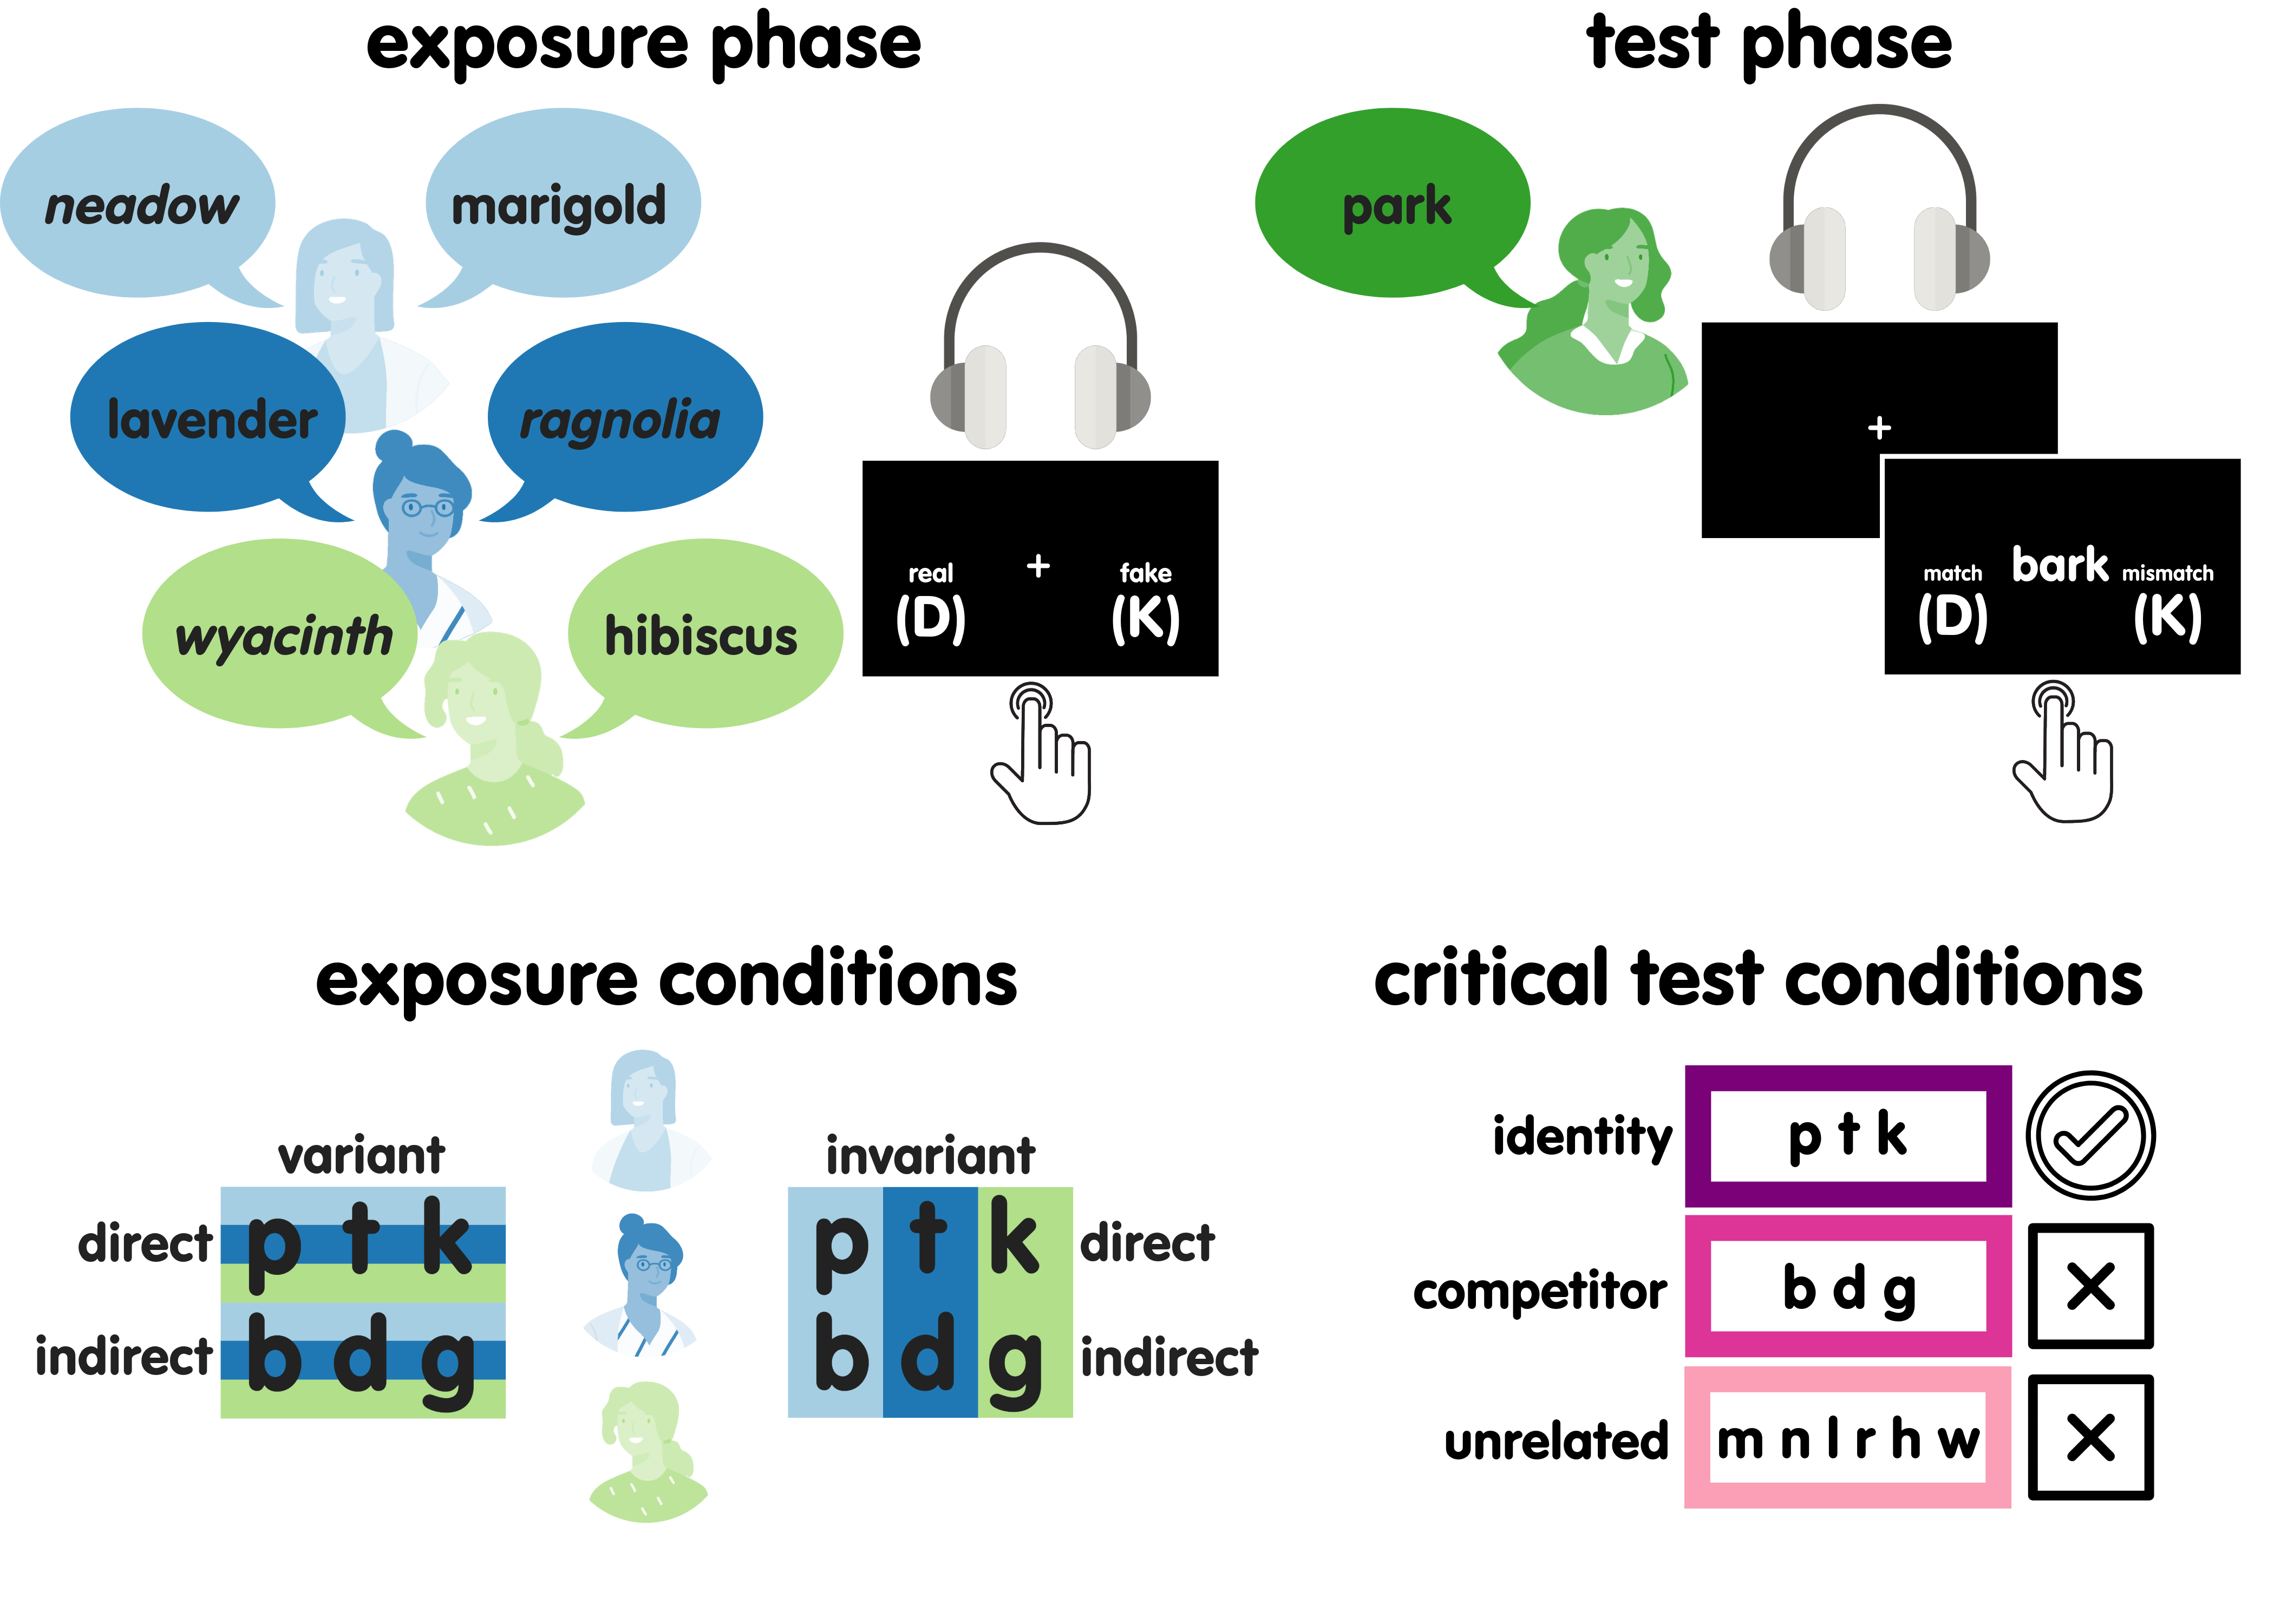
\includegraphics[width=\textwidth]{figures/diss_2} 

}

\caption{Experiment 2 design.}\label{fig:exp2-fig}
\end{figure}

\hypertarget{methods-pars-1b}{%
\paragraph{Participants}\label{methods-pars-1b}}

We recruited 192 participants through Prolific.
After removing ineligible participants, 160 remained.
After removing participants with poor data quality, 154 remained for analysis (Age: \emph{M} = 31, \emph{SD} = 6, Min = 18, Max = 40; Sex: Female = 65, Male = 89; Race: Asian = 5, Black = 17, Multiple selected = 12, Other = 4, White = 116)
All aspects of recruitment were the same as in Experiment 1.
The same group of participants that completed the experiment without the exposure phase in Experiment 1 was also used for comparison.

\hypertarget{materials-and-procedure}{%
\paragraph{Materials and procedure}\label{materials-and-procedure}}

The talkers, stimuli, tasks, and procedure were the same as those in Experiment 1.
Removing the Control level of Similarity from the exposure phase left four between-subjects conditions: Direct-Variant, Direct-Invariant, Indirect-Variant, and Indirect-Invariant.
The 288 filler items remained the same.
The 72 experimental real words also remained the same.
The 72 experimental pseudowords had control onsets regardless of Similarity.
Talker assignment and counterbalancing was the same.
This resulted in 16 experimental lists for the exposure phase, one for each combination of exposure condition (4) and talker assignment (4).
All aspects of the test phase remained the same.

\hypertarget{analysis-and-predictions}{%
\paragraph{Analysis and predictions}\label{analysis-and-predictions}}

Data processing, model fitting, and analysis all remained the same relative to Experiment 1; the only change was implementing sum contrasts for the two levels of Similarity.
Prior to analyzing exposure task performance for real words with experimental onsets, we removed responses with RTs less than 50 ms (\emph{N} = 30; 0.09\%).
We then detected and removed outliers (\emph{N} = 1545; 4.65\%).
Prior to analyzing test task performance for critical prime-target pairs, we removed responses with RTs less than 50 ms (\emph{N} = 7; 0.05\%).
We then detected and removed outliers (\emph{N} = 679; 4.94\%).
For the test task analyses, effect sizes for pairwise comparisons were calculated with the \emph{emmeans} package (Lenth, 2022).

\hypertarget{results-1}{%
\subsubsection{Results}\label{results-1}}

\hypertarget{exposure-1}{%
\paragraph{Exposure}\label{exposure-1}}

There were no effects of Variability or Similarity on accuracy.
There was a main effect of Similarity on RTs (\(\chi^2\)(1, \emph{N} = 2) = 13.86, \emph{p} \textless{} .001), with faster RTs in Indirect conditions (\emph{M} = 1114, 95\% CI {[}1083, 1147{]}) than in Direct conditions (\emph{M} = 1208, 95\% CI {[}1172, 1247{]}; \emph{z} = 3.72, \emph{p} \textless{} .001).

\hypertarget{test-1}{%
\paragraph{Test}\label{test-1}}

For accuracy, we observed a significant interaction between Exposure and Target (\(\chi^2\)(8, \emph{N} = 9) = 19.55, \emph{p} = .012).
Pairwise comparisons within each level of Target did not reveal significant differences between the Test-only condition and any of the exposure conditions (\emph{ps} \textgreater{} .05).
To investigate the source of the Exposure-Target interaction, we expanded the pairwise comparisons to include the contrasts between exposure conditions.
Here, we observed improvements in accuracy on Competitor targets, but not on Identity or Unrelated targets, after Direct-Invariant exposure.
The pairwise comparisons for Competitor targets can be found in Table \ref{tab:exp2-test-tab}.
Performance for each target type for each group is illustrated in Figure \ref{fig:exp2-test-fig}
There were no effects of Exposure on RTs (\emph{ps} \textgreater{} .05).

\begin{table}

\caption{\label{tab:exp2-test-tab}Experiment 2 accuracy differences, \textit{z} ratios, and \textit{p} values for contrasts between groups on Competitor targets.}
\centering
\begin{tabular}[t]{l|l|l|l}
\hline
Contrast & Difference (accuracy) & \textit{z} & \textit{p}\\
\hline
Test-only - Direct-Variant & 0.04 & 1.10 & .918\\
\hline
Test-only - Direct-Invariant & -0.05 & 1.44 & .749\\
\hline
Test-only - Indirect-Variant & 0.04 & 0.99 & .918\\
\hline
Test-only - Indirect-Invariant & 0.05 & 1.43 & .759\\
\hline
Direct-Variant - Direct-Invariant & -0.09 & 2.58 & .079\\
\hline
Direct-Variant - Indirect-Variant & -0.00 & 0.10 & .918\\
\hline
Direct-Variant - Indirect-Invariant & 0.01 & 0.35 & .918\\
\hline
Direct-Invariant - Indirect-Variant & 0.08 & 2.46 & .111\\
\hline
Direct-Invariant - Indirect-Invariant & 0.10 & 2.89 & .039\\
\hline
Indirect-Variant - Indirect-Invariant & 0.10 & 0.45 & .918\\
\hline
\end{tabular}
\end{table}

\begin{figure}[H]

{\centering 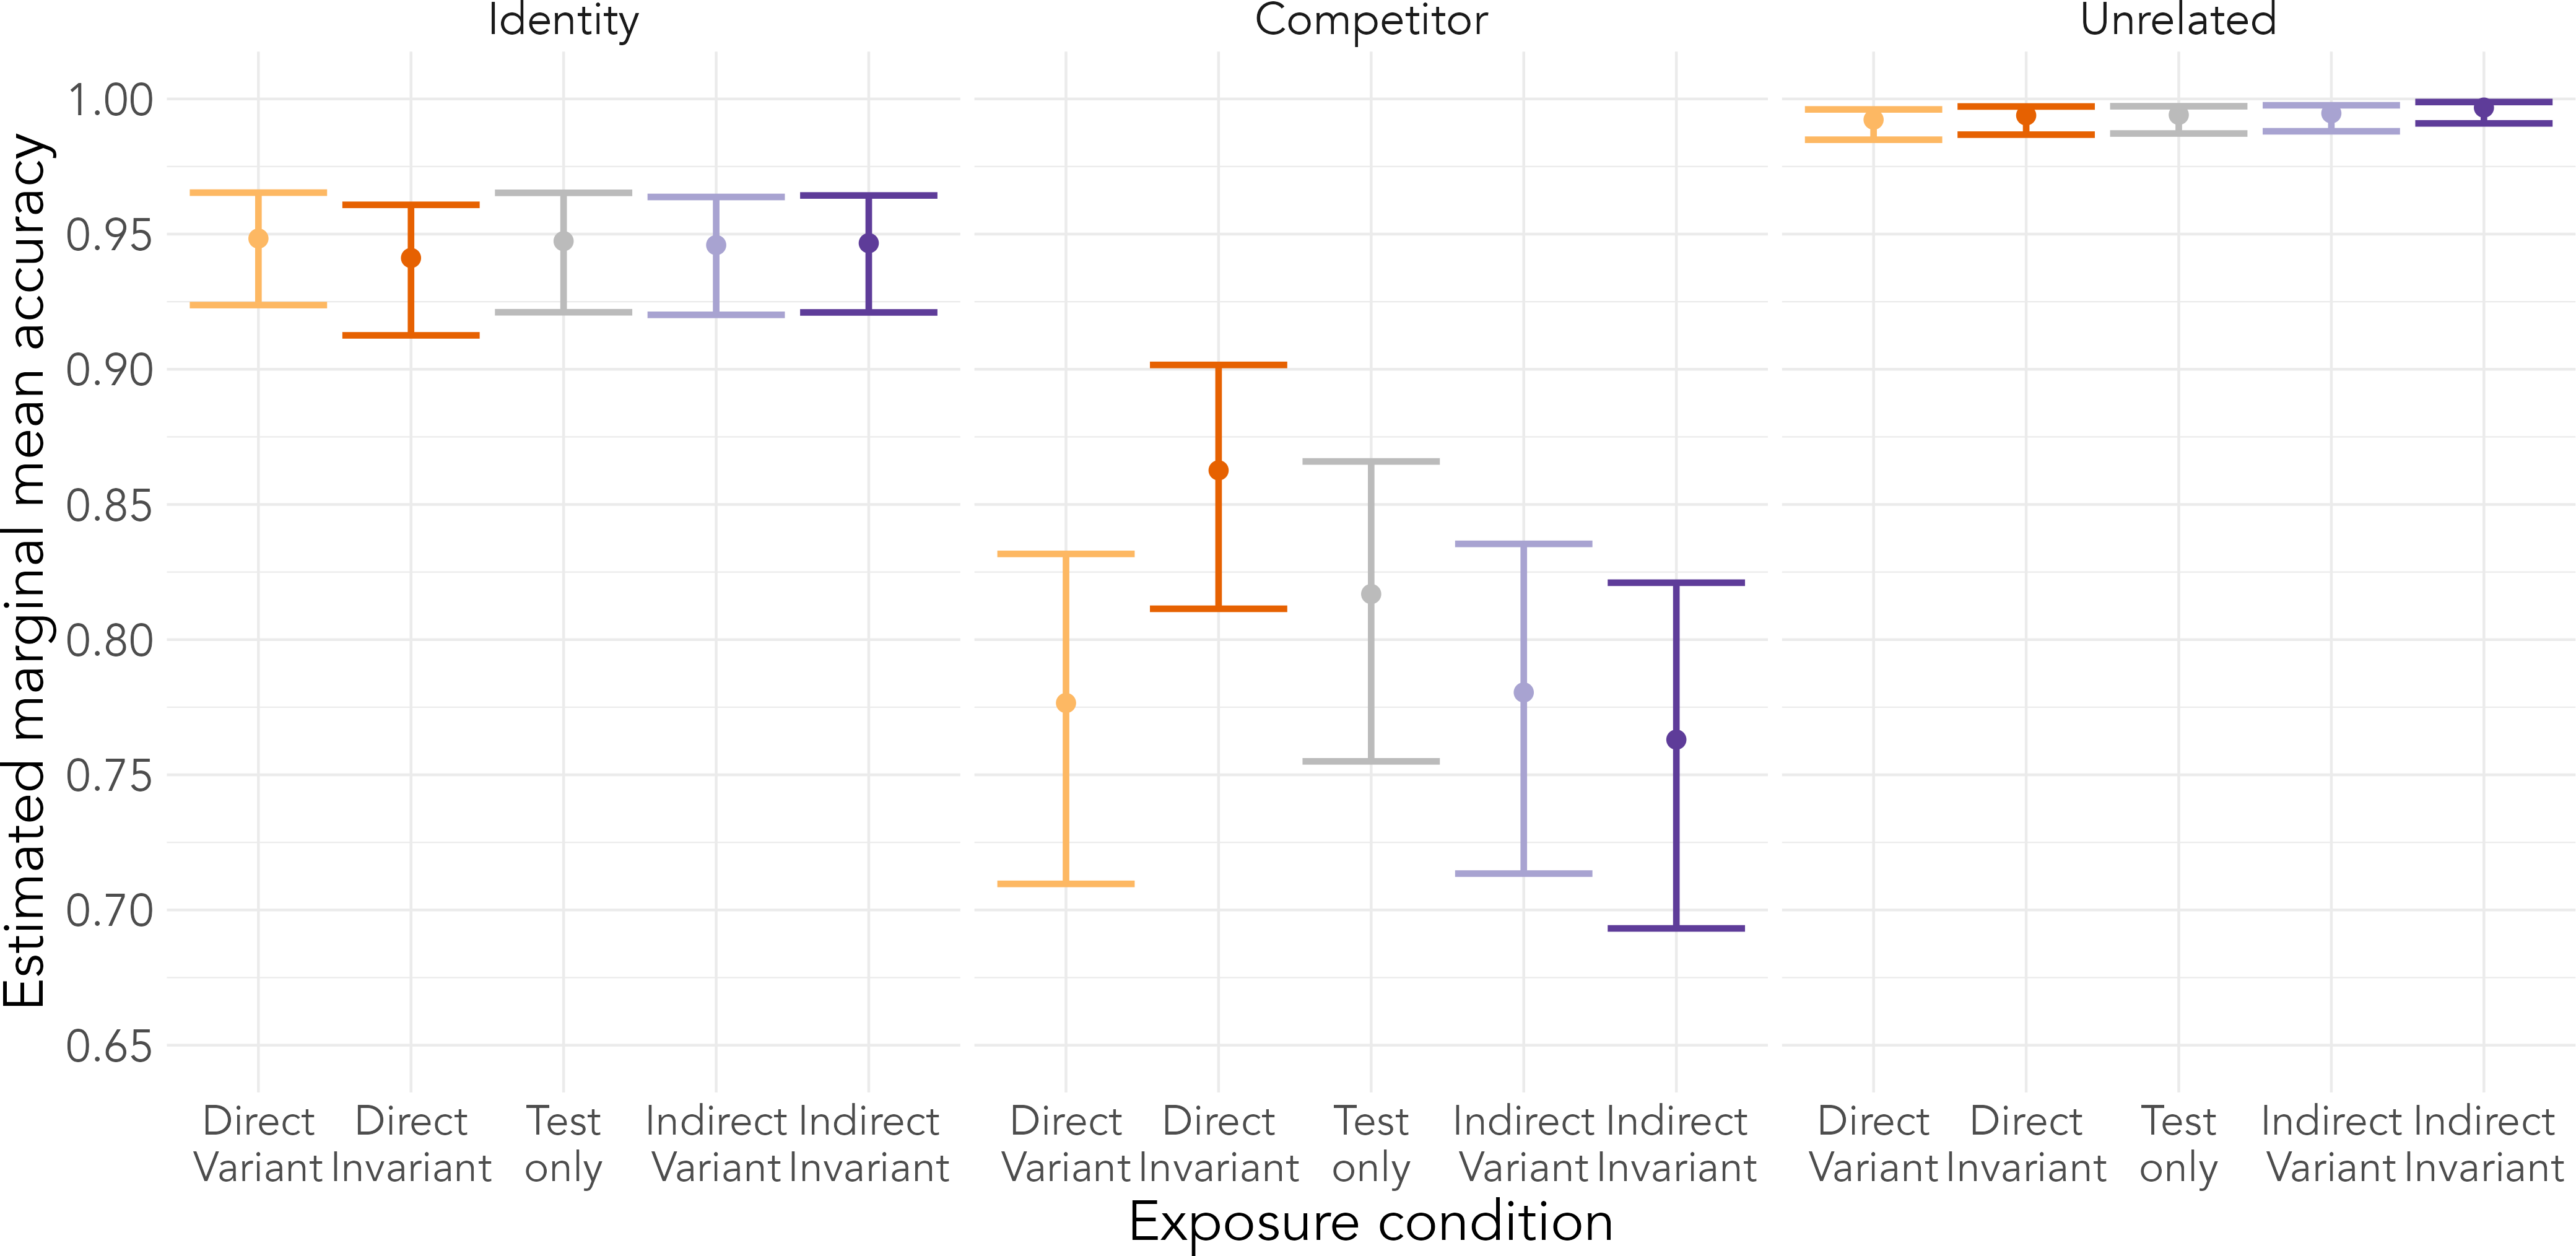
\includegraphics[width=\textwidth]{sections/code/outputs/train_plot_1b} 

}

\caption{Experiment 2 estimated marginal means and 95\% CIs for test accuracy.}\label{fig:exp2-test-fig}
\end{figure}

\hypertarget{discuss-1b}{%
\subsubsection{Discussion}\label{discuss-1b}}

In Experiment 2, two levels of Similarity---Direct and Indirect---were crossed with two levels of Variability---Variant and Invariant---in order to investigate how experience with Spanish-accented stops transfers to a novel talker.
The results of the exposure phase highlight how VOT influences the categorization of stop consonants.
Specifically, participants were faster to accurately categorize real words with voiced stops than with voiceless stops (Indirect exposure versus Direct exposure comparison).
This difference in RT suggests that associating VOTs with voiceless stops was relatively difficult for listeners compared to associating them with voiced stops.
Some of the difference in mean RTs likely reflects the temporal difference between voiced and voiceless stops articulation; however, we did not observe the same difference between Direct and Indirect exposure in Experiment 1, which featured the same real word stimuli.
This suggests that we can attribute the difference in RTs here to the process of learning to map VOT cues onto stop categories.
By contrast, we did not observe main effects of Similarity on accuracy during the exposure phase, which suggests that ultimate categorization did not differ between voiced and voiceless stops.
In other words, even though the \emph{process} of cue-category mapping was more difficult for voiceless stops than for voiced stops, the \emph{outcome} was the same.

This difference in exposure performance translated to a difference in test performance.
While the Direct-Invariant group did not significantly outperform the Test-only group, their performance on Competitor targets was numerically higher.
Moreover, the Direct-Invariant group clearly outperformed the Indirect-Invariant group, trended toward outperforming the Direct-Variant group, and numerically outperformed the Indirect-Variant group.
Together, these results suggest that Direct-Invariant exposure reduced lexical competition between voiced-voiceless minimal pairs.

In order to interpret this finding in terms of generalization, we will briefly describe the structure of the exposure conditions again.
Both Direct conditions exposed participants to Spanish-accented /p/, /t/, and /k/ in such disambiguating lexical contexts as \emph{pencil}, \emph{tablet}, and \emph{kingdom}, respectively.
However, the Direct-Invariant condition in particular exposed participants to one-to-one mappings between each critical onset and each talker, such that all /p/ onsets were produced by Talker A, all /t/ onsets by Talker B, and all /k/ onsets by Talker C.
Thus, participants in the Direct-Invariant group were given the opportunity to develop talker-specific generative models for each VOT-stop mapping.
Recall that a generative model refers to a listener's mental representation of the distribution of a phonetic category (like /p/) over an acoustic cue (like VOT) under the ideal adapter framework.
Since generative models are specific to pairs of cues and categories under this theory, listeners in the Invariant conditions had to organize their representations of VOT for each onset by talker.
By contrast, listeners in the Variant conditions had the option to integrate across talkers to organize each VOT-stop mapping at the accent level, since all three talkers produced exemplars of all onsets.
The fact that Direct-Invariant exposure reduced lexical competition during test means that competition between voiced and voiceless stop contrasts was reduced.
This reduction in perceptual ambiguity was the result of talker-specific generative models for voiceless stops in particular.
Together, these findings suggest that exposure-test similarity is necessary but not sufficient for talker-independent perceptual adaptation; rather, the sources of covariation also need to be reduced during exposure in order for similarity to facilitate generalization.

Finally, we return to the lack of significant differences between the Test-only and Direct-Invariant groups.
The fact that participants without exposure were able to perform at a similar level to those with exposure weakens the argument we put forward in the previous paragraph.
If exposure facilitates generalization, but generalization does not facilitate future performance, then what is the benefit of exposure?
However, there is a wealth of evidence that previous exposure to an L2 accent improves perception of a novel L2-accented talker with the same L1 (Bent \& Baese-Berk, 2021).
Previous studies have generally used either sentence transcription (e.g., Bradlow \& Bent, 2008) or primed lexical decision (e.g., Xie \& Myers, 2017) to test the strength of adaptation.
Here, we used a matching task, under the assumption that categorization of short lag VOTs as voiceless stops should change as a function of perception of short lag VOTs as voiceless stops.
For example, consider the auditory prime \emph{park} and the visual target \emph{bark}.
Participants needed to decide whether the onset of the token they had heard was a /b/ or not.
If they accurately perceived the onset as a /p/, then they would correctly reject \emph{bark} as a match.
Thus, accuracy on the matching task was the outcome of the categorization process.
It is possible that this outcome-based measure was not fine-grained enough to capture subtle changes in perception.
To return to the Competitor target example, the lack of difference in categorizing Spanish-accented \emph{park} as \emph{bark} may belie differences in perceiving Spanish-accented /p/.
To better assess changes in perception, we changed the test task for Experiment 3.

\hypertarget{experiment-3-investigating-fine-grained-perceptual-changes-from-exposure-to-spanish-accented-stops}{%
\subsection{Experiment 3: Investigating fine-grained perceptual changes from exposure to Spanish-accented stops}\label{experiment-3-investigating-fine-grained-perceptual-changes-from-exposure-to-spanish-accented-stops}}

\hypertarget{methods-2}{%
\subsubsection{Methods}\label{methods-2}}

The exposure phase was the same as Experiment 2, but the task used in the test phase was different.

\hypertarget{design-1}{%
\paragraph{Design}\label{design-1}}

To better detect subtle changes in perception as a function of exposure to Spanish-accented speech, we implemented the primed cross-modal lexical decision task from Xie and Myers (2017).
This design is illustrated in Figure \ref{fig:exp3-fig}.
We maintained the same three types of Target: Identity, Competitor, and Unrelated.
However, participants performed a different task with these targets relative to Experiment 2.
Specifically, participants decided whether the visual target was a real English word or not.
The auditory primes should increase or decrease RTs on the visual targets as a function of perceptual adaptation to Spanish-accented voiceless stops.

\begin{figure}[H]

{\centering 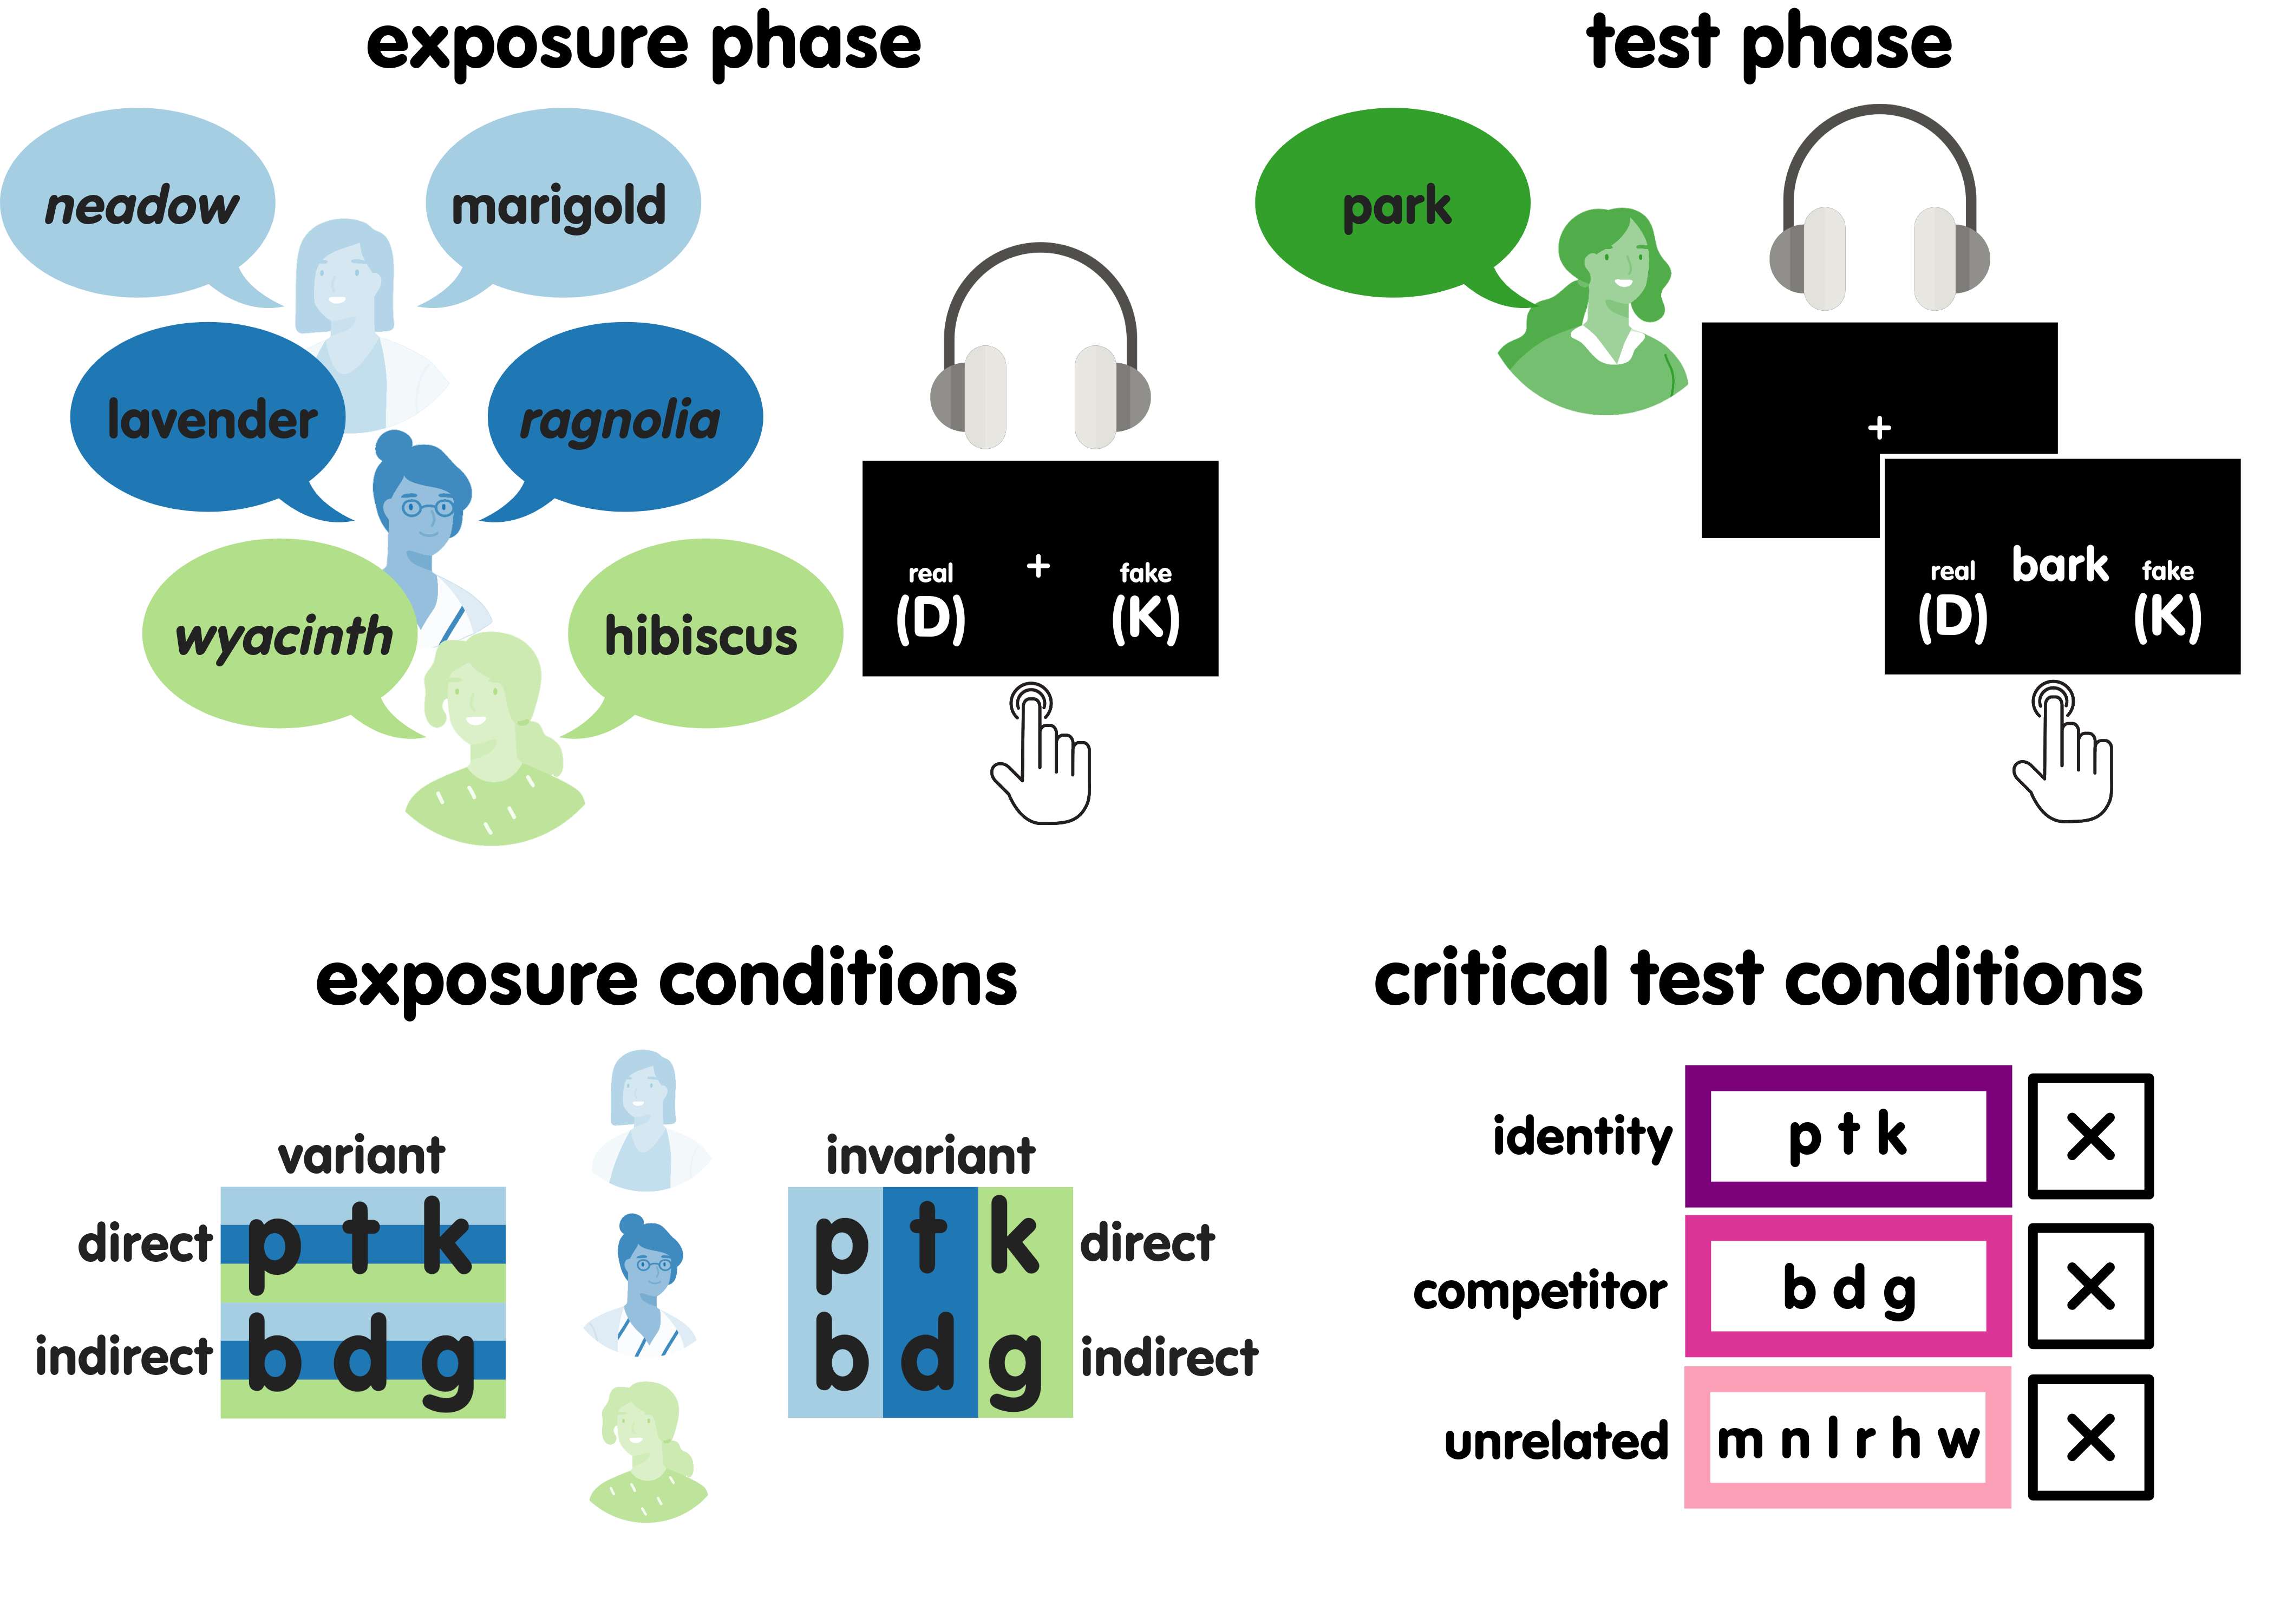
\includegraphics[width=\textwidth]{figures/diss_3} 

}

\caption{Experiment 3 design.}\label{fig:exp3-fig}
\end{figure}

\hypertarget{methods-pars-2}{%
\paragraph{Participants}\label{methods-pars-2}}

We recruited 195 participants through Prolific.
After removing ineligible participants, 170 remained.
After removing participants with poor data quality, 158 remained for analysis (Age: \emph{M} = 31, \emph{SD} = 6, Min = 18, Max = 40; Sex: Female = 80, Male = 78; Race: Asian = 4, Black = 20, Multiple selected = 13, Other = 4, White = 117)
All aspects of recruitment were the same as those described in Experiments 1 and 2.

A separate group of 50 participants was also recruited to complete the experiment without the exposure phase.
There were 43 participants remaining after checking the eligibility criteria, and 42 participants remained after checking for data quality (Age: \emph{M} = 30, \emph{SD} = 5, Min = 21, Max = 40; Sex: Female = 20, Male = 22; Race: Black = 3, Multiple selected = 5, White = 34).

\hypertarget{stimuli}{%
\paragraph{Stimuli}\label{stimuli}}

The real words and pseudowords in the exposure task were the same as those in Experiment 2.
The auditory primes in the test task were also the same.
The only difference was in the visual targets.

The unrelated target for each filler prime (144) was replaced with a pseudoword with a different filler onset from the prime.
Potential pseudowords were downloaded from the ELP's set of normed pseudowords.
The best possible match was selected for each prime by (orthographic) vowel and number of letters.
Three additional pseudoword targets were selected for practice.

\hypertarget{experimental-lists}{%
\paragraph{Experimental lists}\label{experimental-lists}}

The experimental lists for the exposure task were the same as in Experiment 2.
Talker assignment was also counterbalanced the same way.

For the critical primes (72), the combinations of auditory prime and visual target were counterbalanced across participants in three experimental lists as in Experiment 2.
For the filler primes (144), perfect counterbalancing across these three lists was not possible, since three quarters of the filler items in each list (108) needed to have unrelated pseudoword targets.
Three sets of primes, divided evenly by onset, were rotated through the assignment of Identity or Unrelated (pseudoword) target as evenly as possible.
This resulted in 12 experimental lists for the test phase, one for each combination of critical prime-target pair (3) and talker assignment (4).

\hypertarget{tasks-and-procedure}{%
\paragraph{Tasks and procedure}\label{tasks-and-procedure}}

The headphone check, exposure task, and post-experiment questionnaire were the same as Experiment 2.
The procedure was also the same.
The only difference was in the structure of the test task.

The test phase featured the cross-modal primed lexical decision task from Xie and Myers (2017).
On each trial, participants first heard a real word (auditory prime) and then saw a real word or pseudoword written on the screen (visual target).
They indicated whether the visual target was a real English word or not by pressing the \emph{d} or \emph{k} key on their keyboard.
The real word response was mapped to the same key as in the exposure task.
Participants completed six practice trials followed by 216 main trials presented in random order.
Half of the practice trials (3) and half of the main trials (108) required real word responses.
All of the trials with critical primes (72) required real word responses.

\hypertarget{analysis}{%
\paragraph{Analysis}\label{analysis}}

The data processing, model fitting, and analysis approach were the same as in Experiment 2.
Prior to analyzing exposure task performance for real words with experimental onsets, we removed responses with RTs less than 50 ms (\emph{N} = 15; 0.04\%).
We then detected and removed outliers (\emph{N} = 1611; 4.72\%).
Prior to analyzing test task performance for critical prime-target pairs, we removed responses with RTs less than 50 ms (\emph{N} = 53; 0.37\%).
We then detected and removed outliers (\emph{N} = 1076; 7.50\%).

\hypertarget{results-2}{%
\subsubsection{Results}\label{results-2}}

\hypertarget{exposure-2}{%
\paragraph{Exposure}\label{exposure-2}}

There were no effects of Variability or Similarity on accuracy.
There was a main effect of Similarity on RTs (\(\chi^2\)(1, \emph{N} = 2) = 6.09, \emph{p} = .014), with faster RTs in Indirect conditions (\emph{M} = 1107, 95\% CI {[}1075, 1141{]}) than in Direct conditions (\emph{M} = 1169, 95\% CI {[}1134, 1205{]}; \emph{z} = 2.47, \emph{p} = .014).

\hypertarget{first-test-analysis-comparing-the-exposure-groups-to-the-test-only-group}{%
\paragraph{First test analysis: Comparing the exposure groups to the Test-only group}\label{first-test-analysis-comparing-the-exposure-groups-to-the-test-only-group}}

For accuracy, we observed a significant interaction between Exposure and Target (\(\chi^2\)(8, \emph{N} = 9) = 47.48, \emph{p} \textless{} .001); however, pairwise comparisons within each level of Target did not reveal significant differences between the Test-only condition and any of the exposure conditions (\emph{ps} \textgreater{} .05).
We report pairwise differences between exposure conditions in the next analysis.
We also observed a significant interaction between Exposure and Target for RTs (\(\chi^2\)(8, \emph{N} = 9) = 33.56, \emph{p} \textless{} .001).
This interaction was driven by slower RTs on Competitor targets in the Direct-Invariant condition (\emph{M} = 690, 95\% CI {[}654, 730{]}) than in the Test-only condition (\emph{M} = 631, 95\% CI {[}601, 664{]}; \emph{z} = 2.54, \emph{p} = .044).
Pairwise comparisons are shown in Table \ref{tab:exp3-test1-tab} and illustrated in Figure \ref{fig:exp3-test-fig} below.
To investigate the differences between exposure conditions, we conducted the second set of analyses comparing the factors of Variability and Similarity.

\begin{table}

\caption{\label{tab:exp3-test1-tab}Experiment 3 RT differences, \textit{z} ratios, and \textit{p} values for contrasts between the Test-only and exposure groups.}
\centering
\begin{tabular}[t]{l|l|l|l|l}
\hline
Contrast & Target level & Difference (ms) & \textit{z} & \textit{p}\\
\hline
 & Identity & -1 & 0.05 & .959\\
\cline{2-5}
 & Competitor & -6 & 0.31 & .760\\
\cline{2-5}
\multirow{-3}{*}{\raggedright\arraybackslash Test-only - Direct-Variant} & Unrelated & -7 & 0.29 & .775\\
\cline{1-5}
 & Identity & -27 & 1.58 & .454\\
\cline{2-5}
 & Competitor & -59 & 2.54 & .044\\
\cline{2-5}
\multirow{-3}{*}{\raggedright\arraybackslash Test-only - Direct-Invariant} & Unrelated & -56 & 2.23 & .102\\
\cline{1-5}
 & Identity & -15 & 0.88 & .959\\
\cline{2-5}
 & Competitor & -27 & 1.18 & .479\\
\cline{2-5}
\multirow{-3}{*}{\raggedright\arraybackslash Test-only - Indirect-Variant} & Unrelated & -36 & 1.41 & .319\\
\cline{1-5}
 & Identity & 5 & 0.28 & .959\\
\cline{2-5}
 & Competitor & -25 & 1.11 & .536\\
\cline{2-5}
\multirow{-3}{*}{\raggedright\arraybackslash Test-only - Indirect-Invariant} & Unrelated & -47 & 1.85 & .192\\
\hline
\end{tabular}
\end{table}

\hypertarget{second-test-analysis-comparing-the-effects-of-variability-and-similarity}{%
\paragraph{Second test analysis: Comparing the effects of Variability and Similarity}\label{second-test-analysis-comparing-the-effects-of-variability-and-similarity}}

For accuracy, we observed significant two-way interactions between Variability and Target (\(\chi^2\)(2, \emph{N} = 3) = 14.67, \emph{p} \textless{} .001) and between Similarity and Target (\(\chi^2\)(2, \emph{N} = 3) = 25.03, \emph{p} \textless{} .001).
We followed up on these interactions with separate pairwise comparisons for Variability and Similarity within each level of Target.
Within the Identity level of Target, Invariant exposure (\emph{M} = 1.00, 95\% CI {[}0.99, 1.00{]}) was associated with higher accuracy than Variant exposure (\emph{M} = 0.99, 95\% CI {[}0.98, 0.99{]}; \emph{z} = 2.51, \emph{p} = .012).
Within the Competitor level of Target, Indirect exposure (\emph{M} = 0.98, 95\% CI {[}0.96, 0.98{]}) was associated with higher accuracy than Direct exposure (\emph{M} = 0.96, 95\% CI {[}0.94, 0.97{]}; \emph{z} = 2.42, \emph{p} = .016).

\begin{table}

\caption{\label{tab:exp3-test2-tab}Experiment 3 RT differences, \textit{z} ratios, and \textit{p} values for contrasts between exposure groups.}
\centering
\begin{tabular}[t]{l|l|l|l|l|l}
\hline
Contrast & Exposure level & Target level & Difference (ms) & \textit{z} & \textit{p}\\
\hline
 &  & Identity & 25 & 1.41 & .159\\
\cline{3-6}
 &  & Competitor & 53 & 2.17 & .030\\
\cline{3-6}
 & \multirow{-3}{*}{\raggedright\arraybackslash Direct} & Unrelated & 50 & 1.86 & .063\\
\cline{2-6}
 &  & Identity & -20 & 1.07 & .284\\
\cline{3-6}
 &  & Competitor & -3 & 0.10 & .922\\
\cline{3-6}
\multirow{-6}{*}{\raggedright\arraybackslash Invariant - Variant} & \multirow{-3}{*}{\raggedright\arraybackslash Indirect} & Unrelated & 11 & 0.38 & .706\\
\cline{1-6}
 &  & Identity & 31 & 1.71 & .088\\
\cline{3-6}
 &  & Competitor & 35 & 1.33 & .183\\
\cline{3-6}
 & \multirow{-3}{*}{\raggedright\arraybackslash Invariant} & Unrelated & 9 & 0.31 & .758\\
\cline{2-6}
 &  & Identity & -14 & 0.77 & .441\\
\cline{3-6}
 &  & Competitor & -21 & 0.88 & .380\\
\cline{3-6}
\multirow{-6}{*}{\raggedright\arraybackslash Direct - Indirect} & \multirow{-3}{*}{\raggedright\arraybackslash Variant} & Unrelated & -30 & 1.10 & .271\\
\hline
\end{tabular}
\end{table}

For RT, we also observed significant two-way interactions between Variability and Target (\(\chi^2\)(2, \emph{N} = 3) = 13.87, \emph{p} \textless{} .001) and between Similarity and Target (\(\chi^2\)(2, \emph{N} = 3) = 9.05, \emph{p} = .011).
We followed up on these interactions with separate pairwise comparisons for Variability and Similarity within each level of Target; however, the pairwise comparisons between levels of Variability or levels of Similarity were not significant (\emph{ps} \textgreater{} .05).
To further probe the source of the interactions in the model, we conducted pairwise comparisons between Direct and Indirect exposure at each level of Target and Variability and between Variant and Invariant exposure at each level of Target and Similarity.
The results of these analyses can be found in Table \ref{tab:exp3-test2-tab} and are illustrated in Figure \ref{fig:exp3-test-fig}.

\begin{figure}[H]

{\centering 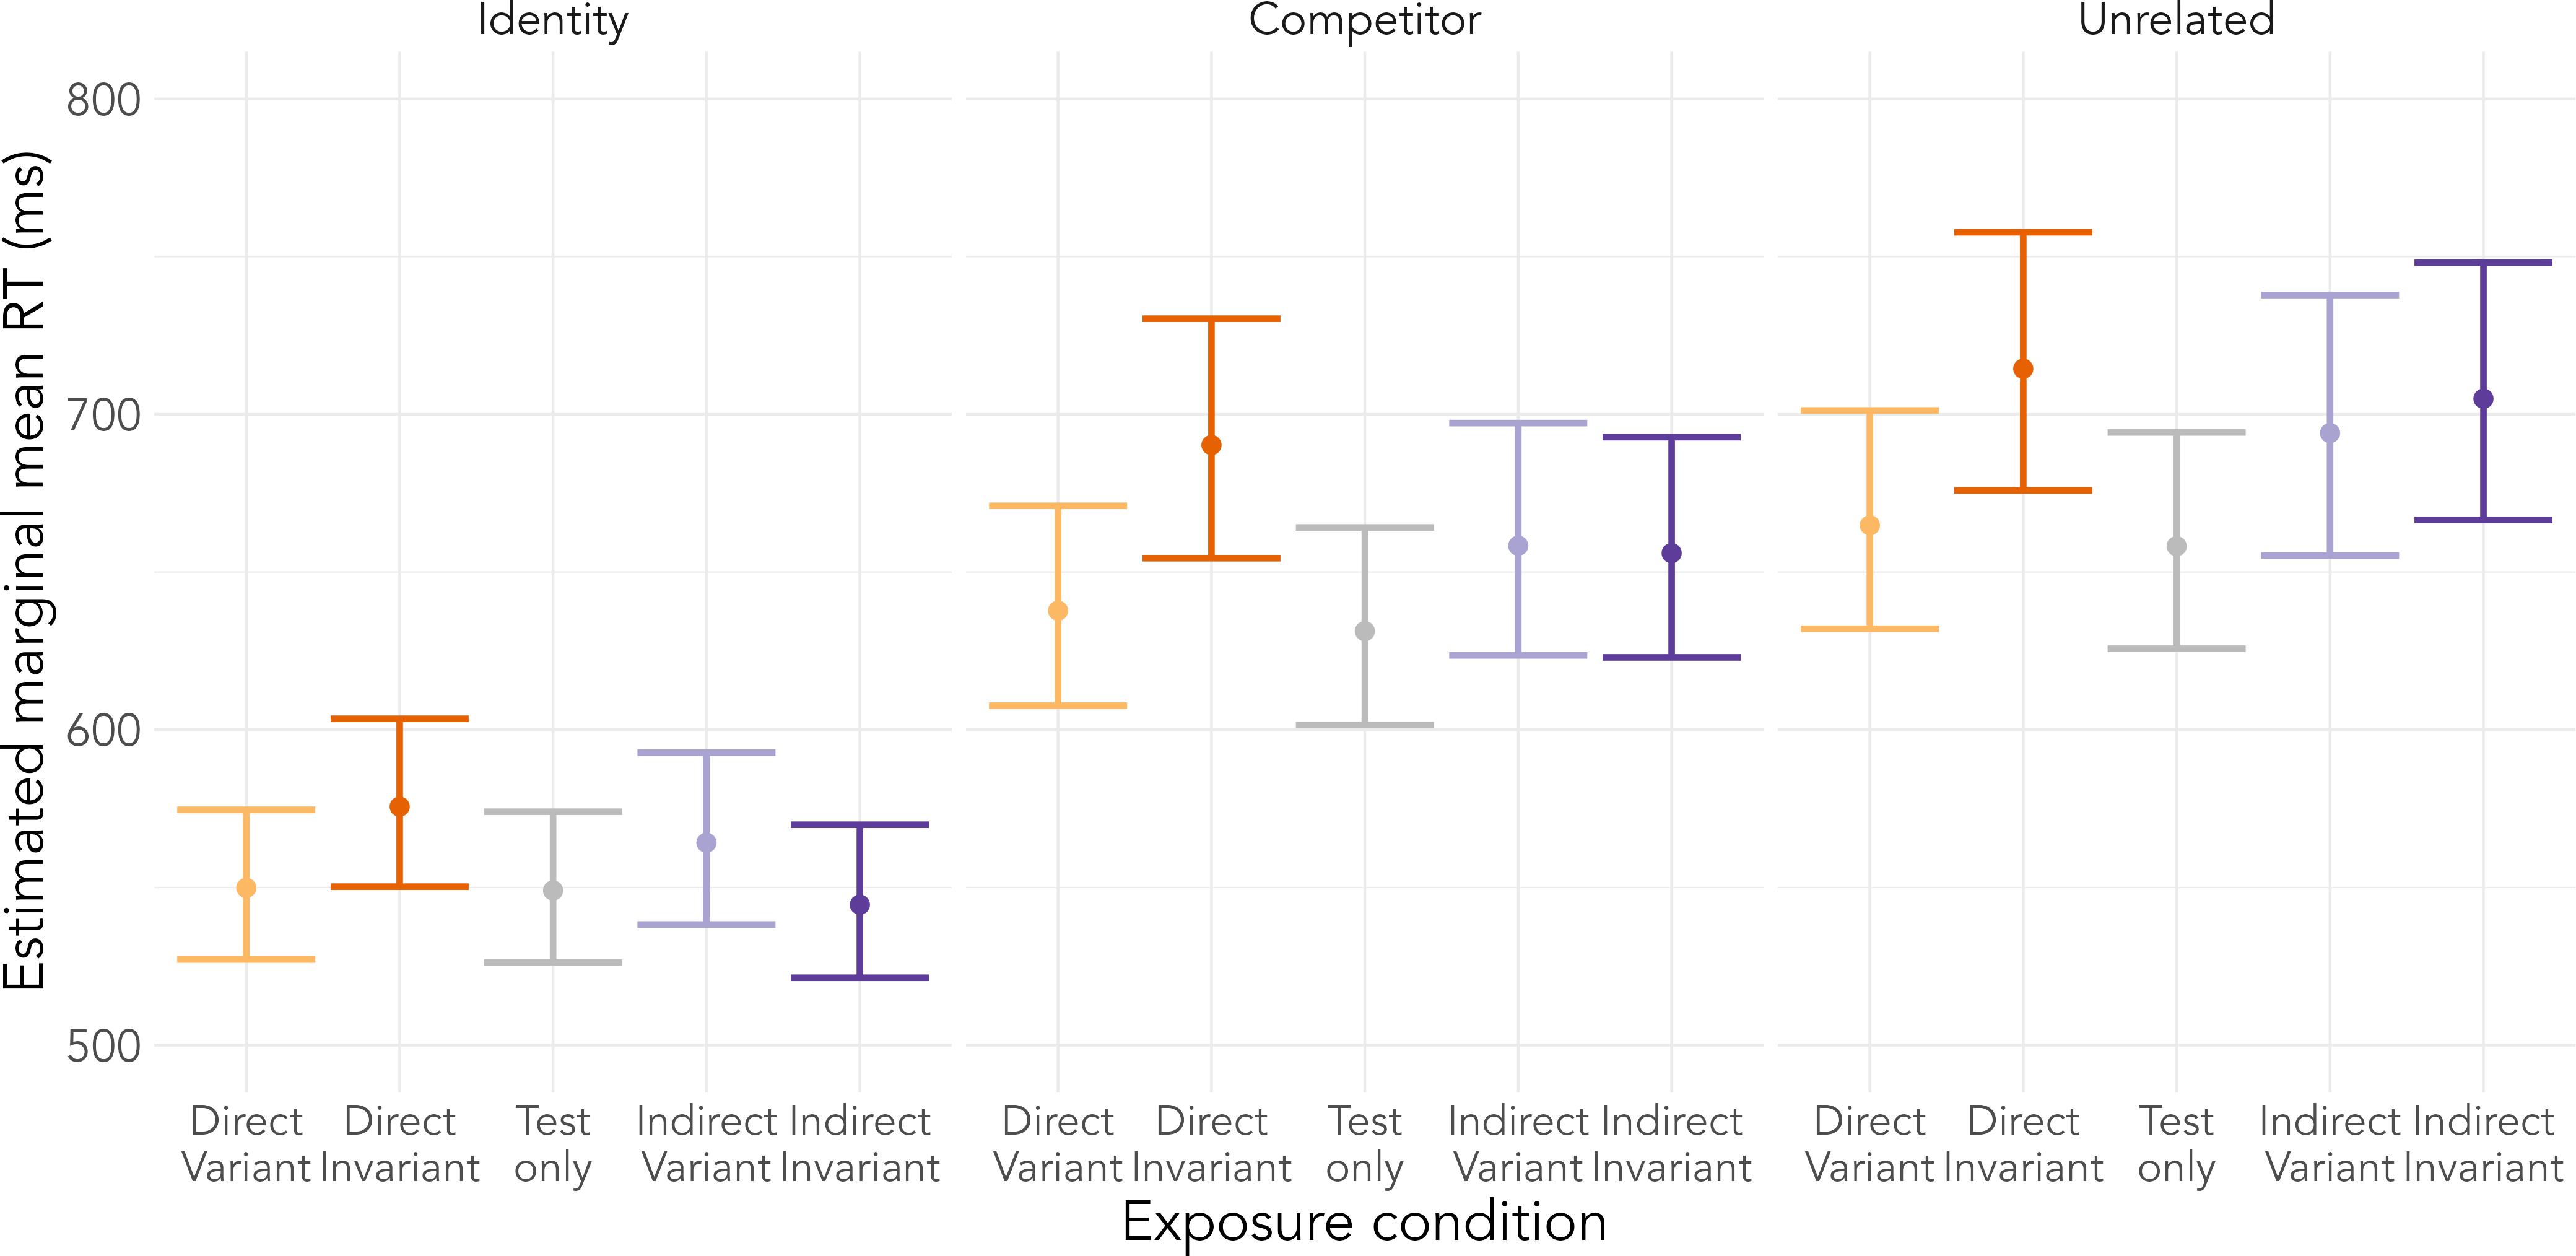
\includegraphics[width=\textwidth]{sections/code/outputs/train_plot_2} 

}

\caption{Experiment 3 estimated marginal means and 95\% CIs for test RT.}\label{fig:exp3-test-fig}
\end{figure}

\hypertarget{discussion-1}{%
\subsubsection{Discussion}\label{discussion-1}}

Experiment 3 followed up on the findings of Experiment 2 with a different test task.
Recall that in Experiment 2, we observed higher accuracy on Competitor targets in the Direct-Invariant group than in any of the other groups.
This difference, however, was only significant for the comparison with Indirect-Invariant training.
The Test-only group performed similarly to the exposure groups, limiting our interpretation of the data.
We posited that Direct-Invariant training reduced lexical competition between voiced and voiceless stops, thereby increasing correct rejection of Competitor targets as matches for the Spanish-accented auditory primes.
The matching task required participants to explicitly compare the visual target to the auditory prime.
In Experiment 3, we took a more implicit approach.
The priming task probed the extent to which the auditory prime activated the visual target.
In this way, we could investigate changes in the perception of Spanish-accented stops.

When we compared the four exposure conditions to the Test-only condition, we observed slower RTs for Competitor targets after Direct-Invariant exposure.
We interpret this reduction in speed as a reduction in lexical competition.
For example, consider the auditory prime \emph{park} and the visual target \emph{bark}, which are minimal pairs that differ only in the voicing of their onsets.
The more the onset of \emph{park} is perceived as /b/, the more it will activate the target \emph{bark}.
This increase in activation will facilitate the lexical decision for \emph{bark}, resulting in faster RTs.
Our results suggest that, in the absence of exposure to Spanish-accented speech, Spanish-accented \emph{park} was perceived \textbf{more} like \emph{bark}.
By contrast, with Direct-Invariant exposure, Spanish-accented \emph{park} was perceived \textbf{less} like \emph{bark}.
This reduction in lexical activation after training suggests that talker-specific exposure to Spanish-accented /p/, /t/, and /k/ improved phonetic categorization of short lag VOTs.
Based on this evidence for talker-independent adaptation, we conducted analyses to distinguish the effects of Variability and Similarity.

Within the Direct conditions, Invariant exposure reduced lexical competition more than Variant exposure.
This effect was illustrated by significantly slower RTs on Competitor targets for the Direct-Invariant group compared to the Direct-Variant group.
In the previous analysis, we also saw that the Direct-Invariant group was slower on Competitor targets than the Test-only group.
This suggests that the Test-only and Direct-Variant groups exhibited similar levels of \emph{park}-\emph{bark} priming, indexing increased activation of /b/ by Spanish-accented /p/.
This finding is striking, considering that the Direct-Variant group had the same amount of exposure to Spanish-accented /p/, /t/, and /k/ as the Direct-Invariant group.
We will interpret this effect of Variability more fully in Section \ref{discuss-study1}.
In short, we will argue that listeners developed sparse talker-specific models rather than more robust talker-independent models during Variant exposure.
Because this level of organization is subject to listeners' use of indexical and social information (Kleinschmidt, 2019), we will investigate their perceptions of the test talker in Section \ref{corr-intro}.

Within the Invariant conditions, Indirect exposure increased lexical activation more than Direct exposure.
This effect was illustrated by marginally faster RTs on Identity targets for the Indirect-Invariant group compared to the Direct-Invariant group.
In other words, previous talker-specific exposure to Spanish-accented /b/, /d/, and /g/ facilitated activation of their voiceless counterparts.
For example, consider the auditory prime \emph{park} and the visual target \emph{park}.
The more the onset of \emph{park} is perceived as /p/, the more it will activate the target \emph{park}.
This increase in activation will facilitate the lexical decision for \emph{park}, resulting in faster RTs.
Our results suggest that, after exposure to Spanish-accented /b/, Spanish-accented \emph{park} was perceived \textbf{more} like \emph{park} than after exposure to Spanish-accented /p/.
This finding was not expected under the exposure-to-variability and similarity-based hypotheses, nor under the ideal adapter framework.
The increase in lexical activation after Indirect-Invariant exposure suggests that experience with the mapping between lead VOTs and voiced stops can facilitate the mapping between short lag VOTs and voiceless stops.
Put another way, exposure to an accent-shifted cue continuum can generalize across both categories and talkers.
We will discuss the reasons for and implications of this finding more thoroughly in Section \ref{discuss-var}.

\hypertarget{corr-intro}{%
\subsection{Correlation analysis}\label{corr-intro}}

Having analyzed the task data, we now compare post-experiment questionnaire responses to test task performance.
Recall that the test task used in Experiments 1 and 2 was different from the one used in Experiment 3.
In both cases, performance on Competitor targets indexed lexical competition.
However, lexical competition had a different relation to performance depending on the task.
For the matching task, accuracy was a direct measure of competition between primes like \emph{park} and targets like \emph{bark}.
Differences in accuracy reflected differences in the activation of the onset competitor \emph{bark}.
RT was less clearly related to differences in activation for competitors (since RT analyses were conducted on accurate responses).
By contrast, for the primed lexical decision task, RT was the clear measure of lexical competition, while accuracy was related more broadly to lexical activation.
Also recall that the test task used in Experiments 1 and 2 did not reveal significant differences between the Test-only and exposure groups.
Considering all of these factors, the correlation analysis presented here only includes the participants from Experiment 3 where we observed differential effects of exposure on test performance.

\hypertarget{corr-mat}{%
\subsubsection{Materials and analysis}\label{corr-mat}}

Here we describe the post-experiment questionnaire items in detail.
The labels for the items in Figure \ref{fig:exp3-corr-fig} are included in parentheses below.

First, participants answered questions related to the test talker's accent.
Participants indicated whether the talker had an accent or not, then rated the strength of the accent (Accent strength) and identified the type of accent.
For the type of accent, participants selected all that applied from the following options: city or region in the US; city or region outside the US; social, racial, or ethnic group; another language; and speech or language impairment.
Responses including the ``another language'' option were coded as 1/2, while responses that did not include this option were coded as -1/2 for analysis (Accent: L2).

Next, participants rated how well they understood the talker (Comprehensibility) and how easy it was to understand the talker (Ease).
They also identified the talker's L1 and proficiency in their L1 (L1 fluency).
Participants selected from the top 10 most spoken languages in the world (Ethnologue, 2024).
Spanish was coded as 1/2 and all other languages were coded as -1/2 (L1: Spanish).
Participants then identified whether the talker was bilingual or not; if so, they identified the talker's L2 and rated their proficiency (L2 fluency).
The same options were provided for identifying the talker's L2, with English coded as 1/2 and the remaining options coded as -1/2 (L2: English).

Finally, participants identified the talker's place of origin.
They began by selecting a global region---Africa, Americas, Asia, Europe, or Oceania---followed by a sub-region within the chosen region (United Nations, 2024).
If the Americas region was selected, participants were also able to select a specific country within their chosen sub-region.
Mexico was coded as 1/2 and all other responses were coded as -1/2 (Country: Mexico).

For the correlations with task performance, we used average RT on Competitor targets as a measure of lexical competition (Competitor RT).
In the primed lexical decision task, RT was a direct measure of competition between minimal pairs, with differences in RT reflecting differences in activation of the onset competitor \emph{bark}.
By contrast, accuracy was less clearly related to differences in activation for competitors, making this measure difficult to interpret in the context of a correlation analysis.
Thus, we did not include Competitor accuracy here.
We also coded participants in the Test-only group as -1/2 and participants in the exposure groups as 1/2 to measure general effects of exposure on test talker judgments (With/out exposure).

Pairwise correlations were calculated with the \emph{psych} package (Revelle, 2023).
A Hommel correction was applied to the \emph{p} values.

\hypertarget{results-3}{%
\subsubsection{Results}\label{results-3}}

All pairwise correlations are illustrated in Figure \ref{fig:exp3-corr-fig}.
None of the questionnaire items correlated with performance on Competitor targets (\emph{ps} \textgreater{} .05).

\begin{figure}[H]

{\centering 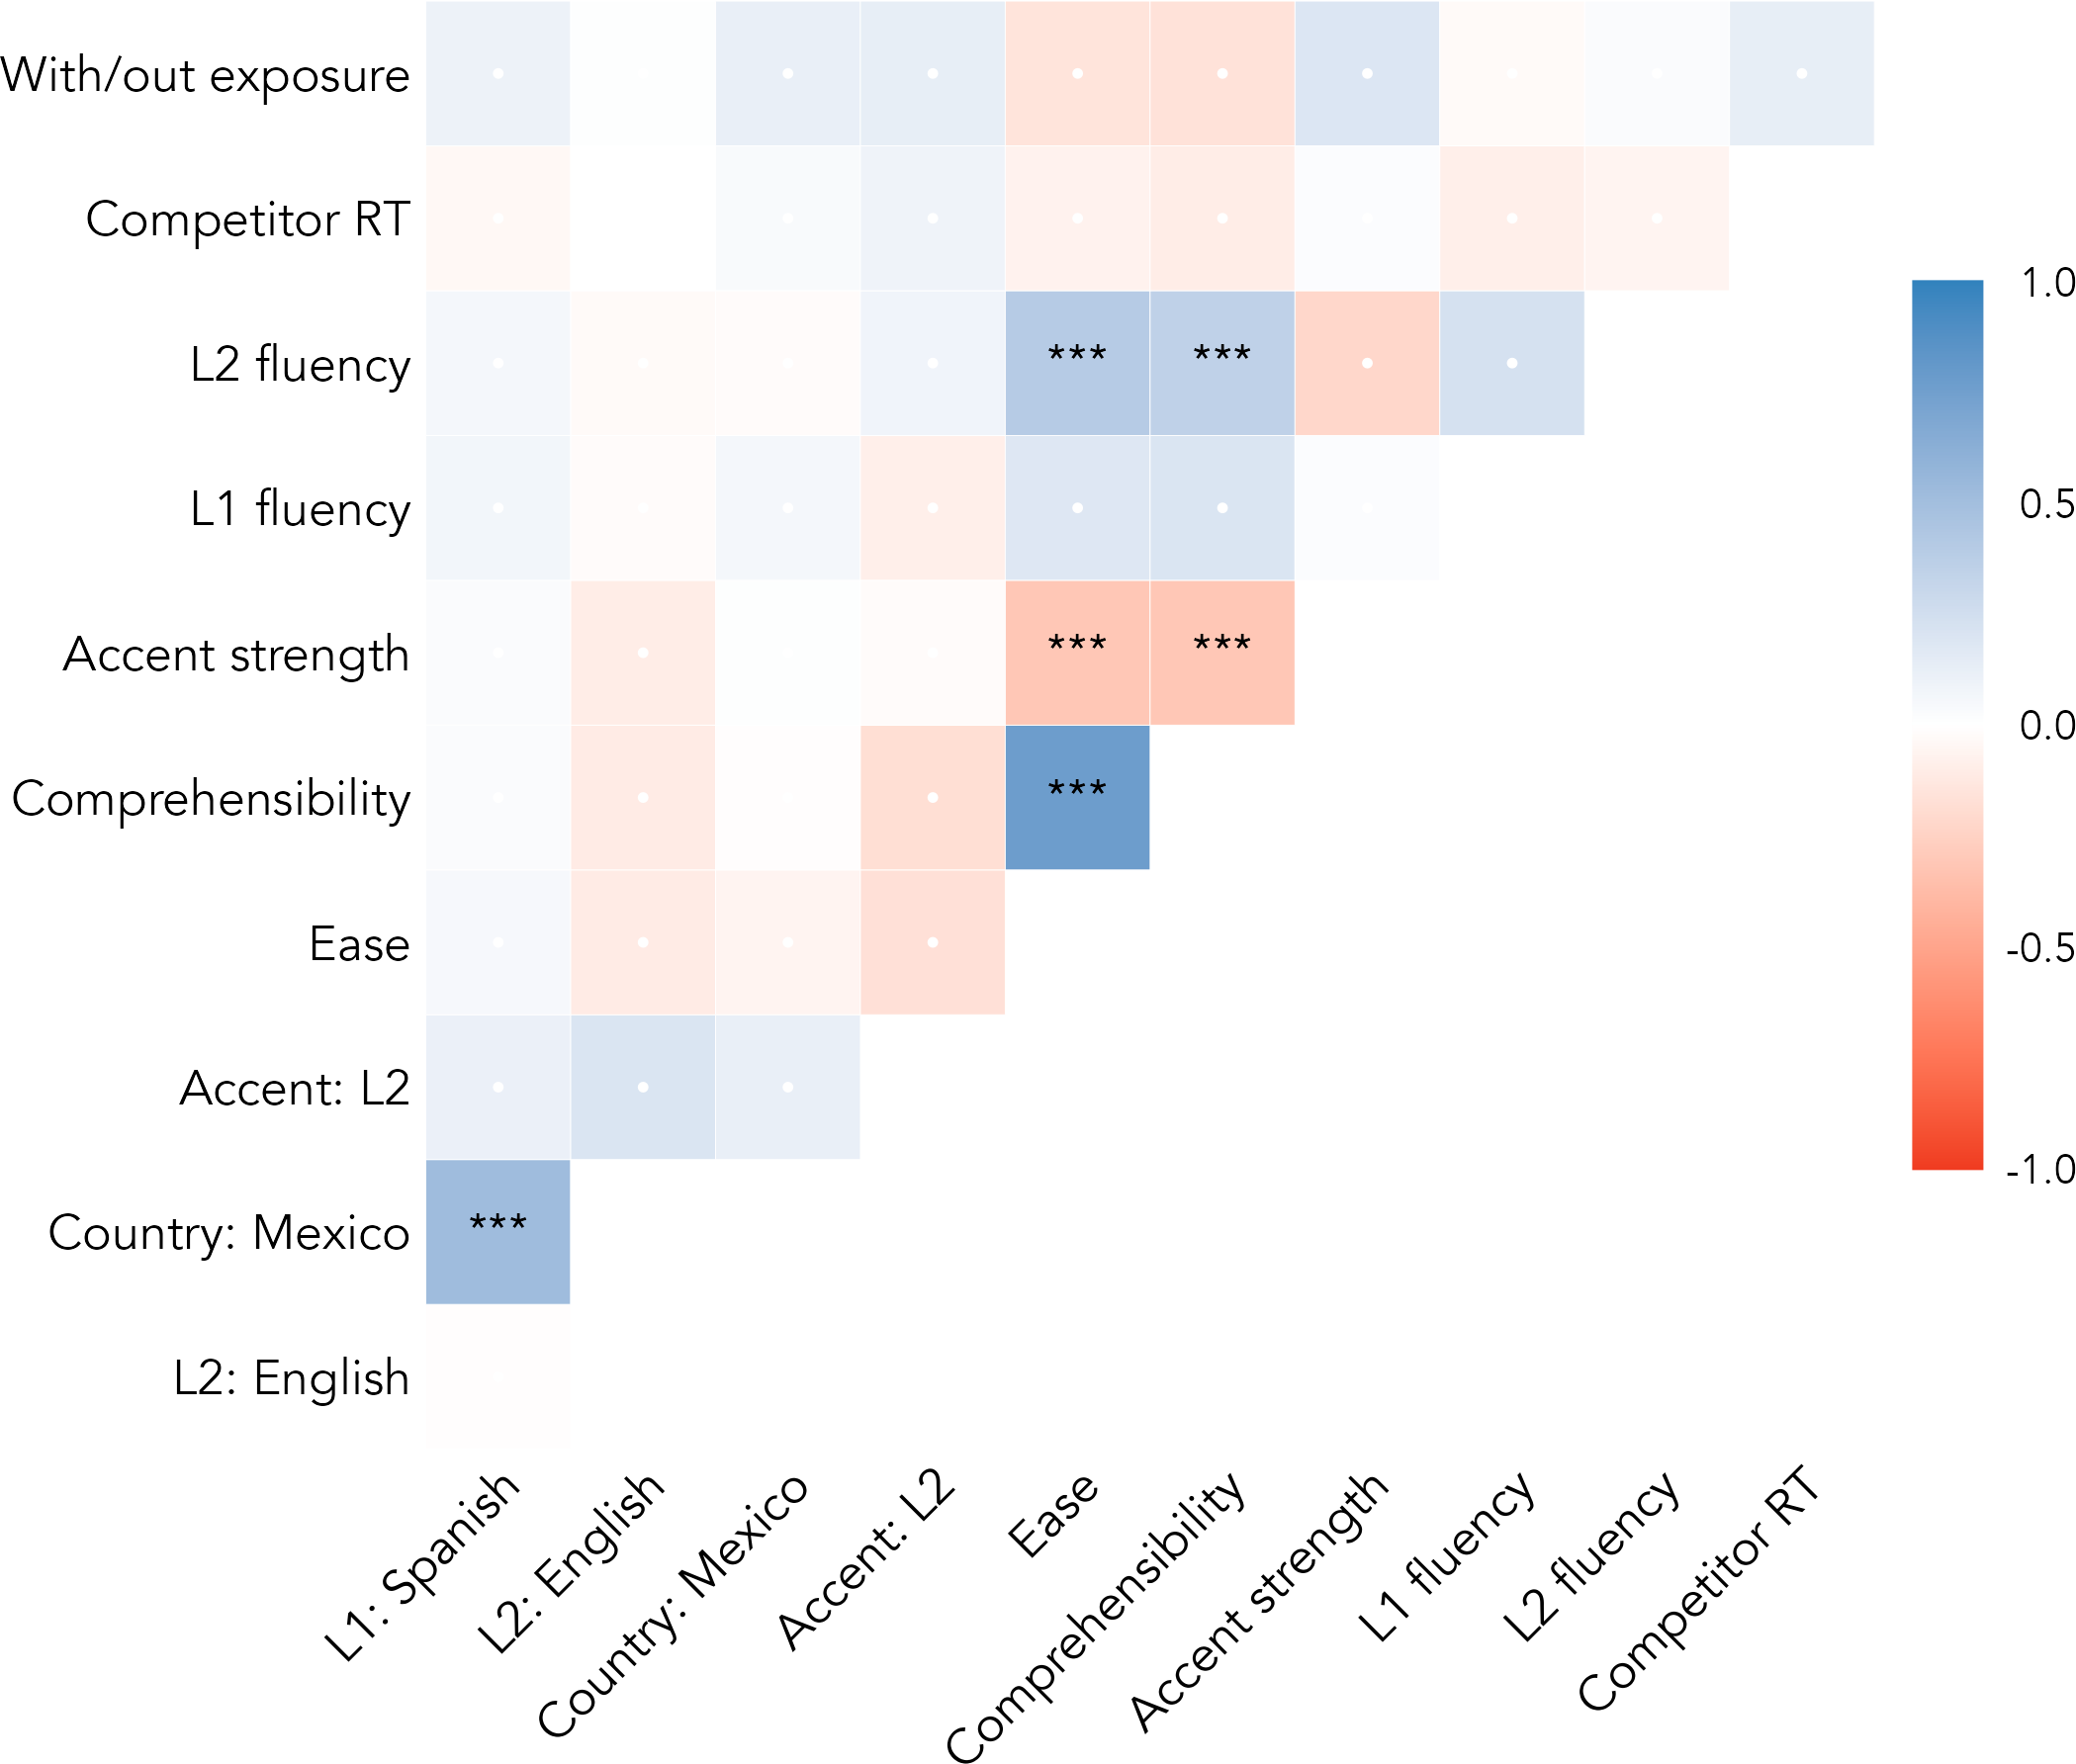
\includegraphics[width=\textwidth]{sections/code/outputs/corr_plot_1} 

}

\caption{Experiment 3 correlation matrix between test performance and post-experiment questionnaire items.}\label{fig:exp3-corr-fig}
\end{figure}

\hypertarget{discussion-2}{%
\subsubsection{Discussion}\label{discussion-2}}

Across participants in Experiment 3, we did not observe any correlations between participant judgments and test performance.
We also did not observe differences between participants who had completed the exposure phase and those who had not.
Within the context of listener perceptions of the talker, ratings of ease, comprehensibility, and accent strength patterned together.
Ease and comprehensibility were also strongly related to ratings of fluency in the L2.
Overall, lexical competition was not particularly sensitive to the social factors we measured.

\hypertarget{discuss-study1}{%
\subsection{General discussion}\label{discuss-study1}}

The current study investigated generalization of exposure to L2-accented speech.
We compared two hypotheses with different explanations for how exposure supports talker-independent adaptation.
The exposure-to-variability hypothesis argues that increasing covariation between acoustic-phonetic cues during exposure increases performance on a new talker (Baese-Berk et al., 2013; Bradlow \& Bent, 2008).
The similarity-based hypothesis argues that increasing cue-category overlap between the exposure and test talkers increases performance on the test talker (Xie \& Myers, 2017).
We expressed these hypotheses in terms of the ideal adapter framework to investigate their explanatory power within the same theoretical model (Kleinschmidt \& Jaeger, 2015).
Under this theory, listeners develop mental models of the mappings between acoustic cues (like VOT) and phonetic categories (like /p/, /t/, and /k/) according to informative and useful social (here, L2 accent) and indexical (talker) groupings (Kleinschmidt, 2019).
To restate the two competing hypotheses using this framework, exposure to variability enhances the formation of talker-independent generative models, while exposure-test similarity facilitates the selection of talker-specific generative models.
Using a novel experimental approach that improved the scope and precision of how variability and similarity are operationalized, a series of three experiments was conducted.
The results provide strongest support for the similarity-based hypothesis and have interesting implications for the ideal adapter framework.

The key findings come from Experiment 3.
After exposure to three Spanish-accented talkers, we measured performance on a novel Spanish-accented talker with a primed cross-modal lexical decision task.
The critical items in this task were monosyllabic auditory primes with voiceless stop onsets: for example, \emph{park}, \emph{tune}, and \emph{coal}.
Importantly, these items had onset competitors with the same place and manner of articulation: \emph{bark}, \emph{dune}, and \emph{goal}, respectively.
Participants made lexical decisions on the visual targets that followed these critical primes.
Performance on the different target types indexed different aspects of perceptual adaptation.
Specifically, priming of Identity targets indexed lexical activation of the intended word, while priming of Competitor targets indexed lexical activation of perceptually similar words.
For example, consider the auditory prime \emph{park}.
The Identity target for this prime is \emph{park}, while the Competitor target for this prime is \emph{bark}.
If perceptual adaptation to Spanish-accented speech increased activation of the lexical item ``park'' upon hearing \emph{park}, then responses to the visual target \emph{park} would also increase.
If perceptual adaptation to Spanish-accented speech decreased activation of the lexical item ``bark'' upon hearing \emph{park}, then responses to the visual target \emph{bark} would also decrease.
Ideally, exposure would both increase activation of the intended word and decrease activation of competing words.
However, we observed differential benefits of exposure on these two processes: Direct-Invariant exposure decreased lexical competition, while Indirect-Invariant exposure increased lexical activation.
Specifically, the Direct-Invariant group displayed significantly slower RTs on Competitor targets than both the Test-only group and Direct-Variant group.
In addition, the Direct-Invariant group displayed marginally slower RTs on Identity targets than the Indirect-Invariant group.
Thus, the decrease in lexical competition we observed was not related to an increase in lexical activation for the intended word.
In the next section, we compare our findings to the predictions of the exposure-to-variability and similarity-based hypotheses.

\hypertarget{exposure-to-variability-versus-similar-exposure}{%
\subsubsection{Exposure to variability versus similar exposure}\label{exposure-to-variability-versus-similar-exposure}}

The exposure-to-variability hypothesis is based on the findings of Baese-Berk et al. (2013).
In that study, exposure to multiple talkers, each with a different L2 accent, generalized to a novel talker with an unfamiliar L2 accent.
Exposure to multiple talkers with the same L2 accent did not generalize to an unfamiliar L2 accent (Bradlow \& Bent, 2008).
However, both types of exposure generalized to a novel talker with a familiar L2 accent.
The multi-accent condition included one Mandarin-accented talker out of five talkers with different L1s, while the single-accent condition included five Mandarin-accented talkers.
In both cases, performance on a novel Mandarin-accented talker was higher than in the control condition.
Together, these results suggest that listeners benefit from exposure to systematic covariation across L2 accents.
In other words, the ways in which L2 varieties differ from L1 varieties at a high level generalizes across L2 talkers.
This hypothesis is also supported by recent work on cross-accent generalization (Bradlow et al., 2023), as well as by the large body of work on high-variability phonetic training for L2 acquisition (for a review, see Zhang et al., 2021).

By contrast, the similarity-based hypothesis comes from Xie and Myers (2017).
In this study, two groups of participants trained on multiple Mandarin-accented talkers.
The experimental group was exposed to disambiguating lexical contexts for word-final /d/ (e.g., \emph{overload}), while the other was not.
During test on a novel Mandarin-accented talker, lexical activation for /d/-final primes was higher in the experimental group.
Among the Mandarin-accented talkers in the training set, one talker's productions of /d/ were similar to those of the test talker on multiple acoustic measures.
There was also one talker out of the five whose productions of /d/ differed from the test talker's on these metrics.
After single-talker exposure to the similar talker, lexical activation for /t/-final competitors was lower in the experimental group.
By contrast, single-talker exposure to the dissimilar talker did not reduce lexical competition.
Overall, single-talker exposure to the similar talker and multi-talker exposure including the similar talker both facilitated generalization to a novel talker.
This suggests that the specific way in which an L2-accented talker instantiates an L2 variety determines the level of generalization to other talkers.
This hypothesis is supported by work on lexically-guided perceptual retuning showing different patterns of generalization for different phonetic contrasts (Kraljic \& Samuel, 2006, 2007; Reinisch \& Holt, 2014).

Having revisited the two competing hypotheses that motivated our work, we return to the specific predictions and results.
The exposure-to-variability hypothesis predicted a main effect of Variability, with better test performance after Variant versus Invariant exposure.
Participants in either condition were also expected to outperform the Test-only group.
This hypothesis does not make predictions regarding activation of intended words (Identity targets) versus activation of competing words (Competitor targets).
However, given that the hypothesis is based on research where transcription accuracy is the measure of generalization, Variant exposure was likely to emerge on Identity target performance.
The similarity-based hypothesis predicted a main effect of Similarity, with better test performance after Direct versus Indirect (or Control) exposure.
Participants in the Direct condition were also expected to outperform the Test-only group.
Specifically, Direct exposure was expected to reduce lexical competition by increasing activation for intended words and decreasing activation for competitors.
Our finding that Direct-Invariant exposure reduced activation of competitors relative to the Test-only group in Experiment 3 supports the similarity-based hypothesis.
We observed this same reduction in lexical competition relative to the Indirect-Invariant group in Experiment 2.
We did not, however, observe a concomitant increase in the activation of intended words after Direct-Invariant exposure in either experiment; in fact, the Indirect-Invariant outperformed the Direct-Invariant group on Identity targets in Experiment 3.
The most striking finding was that the Direct-Variant group outperformed the Direct-Invariant group on Competitor targets in Experiment 3 (and marginally so in Experiment 2).
Together, the differential benefits of Invariant exposure on lexical activation provide direct evidence against the exposure-to-variability hypothesis.
To better understand these findings, we return to how we operationalized Variability and Similarity relative to previous research.

\hypertarget{implementing-similarity}{%
\subsubsection{Implementing similarity}\label{implementing-similarity}}

Across three experiments, we manipulated two key aspects of exposure that are thought to facilitate generalization: variability and similarity.
We took a novel approach to implementing these manipulations compared to previous work (Baese-Berk et al., 2013; Bradlow et al., 2023; Bradlow \& Bent, 2008; Xie et al., 2021; Xie \& Myers, 2017).
Regarding similarity, we exposed different groups of participants to different sets of items in an auditory lexical decision task.
In Direct conditions, participants gained experience with the voiceless stops /p/, /t/, and /k/ in the context of real words like \emph{pencil}, \emph{tablet}, and \emph{kingdom}, respectively.
In Indirect conditions, participants gained experience with the voiced stops /b/, /d/, and /g/ in the context of real words like \emph{beehive}, \emph{desert}, and \emph{gallop}, respectively.
These items provided the context for perceptual adaptation to three Spanish-accented talkers.
Through Direct and Indirect exposure, we operationalized Similarity as the type of information listeners received about the relation between VOT and voiceless stops in Spanish-accented English.

Spanish-accented English was chosen because it differs from L1-accented English in its distributions of contrastive stop voicing over VOT.
Differences in these distributions can disrupt speech perception, because L1 English listeners use VOT as the primary cue to distinguish voiced from voiceless stops in word-initial position.
In L1-accented English, the voiced stops /b/, /d/, and /g/ are produced with short lag VOTs, while the voiceless stops /p/, /t/, and /k/ are produced with long lag VOTs.
For example, consider the bilabial stops /b/ and /p/, which have the same place (bilabial) and manner (stop) of articulation.
L1 English listeners tend to categorize bilabial stops produced with short lag VOTs as /b/.
However, in Spanish-accented English, cross-language transfer shifts the relations between VOTs and stops; as a result, the voiced stops /b/, /d/, and /g/ are produced with lead VOTs, while the voiceless stops /p/, /t/, and /k/ are produced with short lag VOTs.
The tendency for L1 English listeners to categorize short lag VOTs as voiced, while optimal for L1-accented speech, is sub-optimal for Spanish-accented speech.
In order to correctly categorize Spanish-accented voiceless stops, L1 listeners must learn to associate short lag VOTs with /p/, /t/, and /k/ rather than with /b/, /d/, and /g/.
There are two ways that listeners could achieve this outcome.
First, exposure to short lag VOTs in disambiguating lexical contexts like \emph{pencil} would train listeners to shift the VOT distribution for voiceless stops from long lag to short lag for Spanish-accented talkers.
This is the logic behind the Direct exposure conditions.
Second, exposure to lead VOTs in supporting lexical contexts like \emph{beehive} would train listeners to shift the VOT distribution for voiced stops from short lag to lead.
Shifting the VOT distribution for voiced stops leftward on the cue continuum could trigger a more general leftward shift, moving the VOT distribution for voiceless stops from long lag to short lag.
This is the logic behind the Indirect exposure conditions.

This way of investigating similarity differs from that of Xie and Myers (2017).
Their key manipulation related to the /t/-/d/ voicing contrast in Mandarin-accented English.
In word-final position, voiceless stops are distinguished from voiced stops by the duration of the preceding vowel.
For L1 listeners of English, longer vowel durations are associated with voiced stops.
However, in Mandarin-accented English, vowels are shortened before voiced stops, making voiced stops perceptually confusible with voiceless stops.
This is illustrated by the minimal pair \emph{seed}-\emph{seat}, where shortening the vowel before /d/ makes \emph{seed} sound like \emph{seat}.
There are also two secondary cues to voicing in this position: burst duration and closure duration.
Xie and Myers (2017) compared each talker's mean values for vowel, burst, and closure duration on word-final /d/ with t-tests.
The dissimilar talker differed significantly on all three measures, while the similar talker did not.
Thus, similarity was operationalized as a between-talker comparison.
While our approach did not take this kind of fine-grained acoustic-phonetic similarity into account, it did allow us to use the same exact talkers between conditions.
In this way, we were able to control between-talker sources of acoustic-phonetic variability across levels of Similarity.
This was important for manipulating variability independent of similarity.
A by-product of this choice, however, was that we did not control the exact VOT-stop distributions that listeners heard during exposure.
If these distributions were not as close of a match as they were between Xie and Myers (2017)'s exposure and test talkers, this would explain why lexical activation of the primes was not enhanced by Direct training even though it reduced competition.

\hypertarget{discuss-var}{%
\subsubsection{Implementing variability}\label{discuss-var}}

Regarding variability, we exposed different groups of participants to different combinations of talker and onset.
In Variant conditions, participants gained experience with the VOT distributions for each onset across talkers.
Since there were 24 real word stimuli per onset, this means that each of the three talkers produced eight experimental items with each onset.
In Invariant conditions, participants gained experience with the VOT distributions for each onset within talkers.
This means that each talker produced 24 experimental items with a single onset.
The variability manipulation was also extended to the filler items, with two filler onsets assigned to each talker.
Overall, listeners heard 72 real words from each talker during exposure.
By contrast, in Bradlow and Bent (2008) and Baese-Berk et al. (2013), participants in the multi-talker exposure groups heard 16 sentences with 50 total key words per talker.
While each set of sentences was different for each exposure talker, participants completed five repetitions per talker, increasing the total amount of exposure to each talker to 250 key words.
This is nearly three times the amount of word-level exposure to each talker compared to our study.
Previous research has shown that listeners need significantly more exposure to adapt to multiple talkers compared to a single talker (Luthra et al., 2021).
Even in a talker-specific paradigm, test performance increases with increasing evidence for adaptation (Cummings \& Theodore, 2023).
Thus, the relatively limited amount of exposure our participants had to variability may have limited the strength of its benefits.
However, the amount of exposure did not differ between our levels of Variability.
Moreover, we observed a clear benefit for Invariant versus Variant exposure.
We interpret this finding in terms of the specificity of generative models.

According to Kleinschmidt (2019), generative models can be constructed according to an individual person (talker-specific) or a higher-level social category (talker-independent).
The level of organization is determined by two factors.
First, the model needs to be a good representation of the actual distribution.
That is, the cue-category mappings that the listener has heard so far need to be captured by the mental representation.
Second, the model needs to be a good predictor of future exemplars.
In other words, the mental representation needs to help listeners categorize a given instance of a cue as a particular category.
In our experiment, we gave listeners different samples of each talker's VOT distributions.
We can illustrate this idea with Talker A and her VOT-/p/ mapping.
Variant exposure gave listeners a small sample of Talker A's VOT-/p/ mapping relative to Invariant exposure, where all VOT-/p/ mappings were from Talker A.
Direct exposure allowed listeners to sample Talker A's VOT distribution for /p/, while Indirect exposure only allowed listeners to sample her VOT distribution for the voiced counterpart /b/.
These different samples influenced how listeners constructed their representations.

As explained in Section \ref{discuss-1b}, talker-specific generative models were the only possible representations of Invariant exposure.
This is because Invariant exposure only provided one talker's cue distributions for a given category.
With Variant exposure, both talker-specific and talker-independent models were possible; however, talker-independent models were optimal.
This is because there were only 24 exemplars of each phonetic category divided among three talkers.
Thus, talker-specific models would have been developed from a relatively sparse sample.
If we assume that the talkers had similar VOT-stop distributions, the talker-specific generative models developed during Invariant exposure should have been as useful as the talker-independent generative models developed during Variant exposure.
However, the reduction in lexical competition following Direct-Invariant exposure compared to Direct-Variant exposure in Experiments 2 and 3 suggests that this was not the case.
There are two possible explanations: first, the talker-independent models from Variant exposure were not as useful as the talker-specific models from Invariant exposure; second, listeners developed talker-specific models during Variant exposure, which were not as useful as a talker-independent model would have been.
Both of these explanations could be the result of different VOT distributions for each talker.
This would also explain why Direct-Invariant exposure did not increase Identity priming as discussed in the previous section.

Socio-indexical organization cannot, however, explain why Indirect-Invariant exposure increased Identity priming relative to Direct-Invariant exposure in Experiment 3.
Increased lexical activation of primes like \emph{park} after exposure to words like \emph{beehive} is evidence for both talker-independent and category-independent adaptation.
Indirect-Invariant training exposed listeners to Talker A's VOT-/b/ distribution, Talker B's VOT-/d/ distribution, and Talker C's VOT-/g/ distribution.
By comparison, Direct-Invariant training exposed listeners to Talker A's VOT-/p/ distribution, Talker B's VOT-/t/ distribution, and Talker C's VOT-/k/ distribution.
When tested on Talker D, listeners in the Indirect-Invariant group showed stronger lexical activation for primes with /p/, /t/, and /k/ onsets.
In other words, exposure to voiced stops improved perception of voiceless stops, but only when each stop was produced by a different talker.
This finding was not expected under the ideal adapter framework, where adaptation is specific to a given phonetic category, nor by the exposure-to-variability or similarity-based hypotheses.
It is also counter to the findings of Clarke and Luce (2005), where training on modified VOT continua for /t/ and /d/ did not generalize to /k/ and /g/ (see also Eisner \& McQueen, 2005).
However, our results do align with those of Kraljic and Samuel (2006), who demonstrated generalization from a /t/-/d/ continuum to a /p/-/b/ continuum (see also Kraljic \& Samuel, 2007).
Overall, the conditions under which perceptual adaptation generalizes to other phonetic categories requires further research.

\hypertarget{conclusion}{%
\subsubsection{Conclusion}\label{conclusion}}

Overall, our results show that talker-independent adaptation to L2-accented speech is facilitated by exposure-test similarity.
We also found evidence that generalization is enhanced when variability is limited, at least for the rapid adaptation effects we investigated here.
This study is the first to compare variability and similarity while maintaining the same talkers across conditions.
This level of control is key to understanding how exposure to between-talker variability interacts with exposure to specific acoustic-phonetic properties.
We suggest that the contradictory findings in the literature are at least partially a result of comparing different talkers, who have idiosyncratic patterns of within-talker covariation (Clayards, 2017; Whalen et al., 2018; Xie \& Jaeger, 2020).
Listeners are highly sensitive to variation in speech, particularly during perception.
In future work, we hope to better understand how this sensitivity is deployed during talker- and category-independent adaptation to L2-accented speech.

\newpage

\hypertarget{study-2-the-neurocognitive-correlates-of-talker-specific-adaptation-to-spanish-accented-english}{%
\section{Study 2: The neurocognitive correlates of talker-specific adaptation to Spanish-accented English}\label{study-2-the-neurocognitive-correlates-of-talker-specific-adaptation-to-spanish-accented-english}}

\hypertarget{introduction-1}{%
\subsection{Introduction}\label{introduction-1}}

Models of speech recognition ground high-level accent adaptation in low-level acoustic-phonetic processes.
The ideal adapter framework in particular posits that listeners use statistical learning to develop mental representations of the probabilistic mappings between acoustic cues and phonetic categories (Kleinschmidt \& Jaeger, 2015).
This model accounts for the wealth of behavioral data on talker-specific adaptation (e.g., Bradlow \& Bent, 2008; Clarke \& Garrett, 2004; Xie et al., 2017, 2018, 2021).
A typical experimental design features two phases: the first phase exposes the participant to the talker, while the second phase tests what the participant has learned about the talker.
Across studies, exposure to a talker's cue-category mappings during the first phase leads to faster and more accurate responses on the same talker in the second phase compared to a different talker.
The effects of perceptual adaptation on neural signatures are less clear.
Neurocognitive studies of L2-accented speech processing have not typically been designed to induce adaptation through the systematic manipulation of stimulus materials.
Rather, adaptation effects have mainly been investigated by comparing mean responses in each experiment half (Gosselin et al., 2021; Hanulíková et al., 2012; Romero-Rivas et al., 2015).
For example, Romero-Rivas et al. (2015) demonstrated a reduction in the neural correlates of lexico-semantic processing with exposure to L2-accented speech.
Such analyses have yielded little evidence for adaptation, despite the large body of evidence for adaptation to L2-accented speech in studies using behavioral measures.
The present study takes a different approach to investigating the neurocognitive correlates of adaptation with a novel experimental design.
This approach takes the exposure-test design common in the behavioral literature and integrates the two phases to measure real-time changes in adaptation to an L2-accented talker.

Our study leverages the predictions of the ideal adapter framework to explore the neurocognitive mechanisms that support perceptual adaptation to L2-accented talkers.
We focus on one acoustic cue---VOT---and its association with the phonetic categories /p/, /t/, and /k/ in Spanish-accented speech.
Voiceless stop consonant VOT in Spanish-accented English was chosen as the focus of the present study for several reasons.
Firstly, VOT is relatively easy to measure and manipulate from a researcher's perspective (Winn, 2020).
Secondly, variation in VOT affects both L1 word recognition (Andruski et al., 1994; Utman et al., 2000) and L2 accent categorization (McCullough \& Clopper, 2016).
Thirdly, and most importantly for our investigation of L2-accented speech, the mappings between VOT as an acoustic cue and voiceless stops as phonetic categories vary cross-linguistically between English and Spanish (Campos-Astorkiza, 2012; Lisker \& Abramson, 1964).
We take advantage of L1-L2 transfer in the production of voiceless stop VOTs to investigate adaptation to a Spanish-accented English talker.

\hypertarget{erp-correlates-of-acoustic-phonetic-processing}{%
\subsubsection{ERP correlates of acoustic-phonetic processing}\label{erp-correlates-of-acoustic-phonetic-processing}}

Electroencephalography (EEG) captures voltage changes associated with neural activity with millisecond-by-millisecond precision (Luck, 2014).
The event-related potential (ERP) analysis technique, which timelocks the EEG signal to the onset of a stimulus, takes advantage of this excellent temporal resolution to isolate the neurocognitive mechanisms that support specific linguistic processes.
ERPs are relative measures, meaning that two or more conditions need to be compared in order to interpret the effects.
The amount of time between the onsets of two conditions and the emergence of amplitude differences is thought to be directly related to the time-course of language processing.

During comprehension, acoustic-phonetic processing precedes lexico-semantic access, both conceptually in psycholinguistic theories (Marslen-Wilson, 1984; McClelland \& Elman, 1986; Norris, 1994) and physically in the EEG signal (Hagoort, 2017).
The earliest cortical response to auditory stimuli is the negative-going N1 component, which peaks at approximately 100 ms post stimulus onset in frontal channels and indexes acoustic processing.
Phonetic processing is associated with the positive-going P2/P200 component, which typically peaks between 150 and 250 ms post stimulus onset in central and fronto-central channels.
Together, these two components form the N1-P2 complex, which indexes the engagement of selective attention during perception (Hillyard et al., 1973; Joos et al., 2014; Sanders \& Astheimer, 2008).
Lexico-semantic processing is indexed by the N400 component, a negative-going waveform peaking at approximately 400 ms post stimulus onset across centro-parietal channels (Federmeier, 2021; Kutas \& Hillyard, 1984).
The negative-going N200/PMN (phonological mapping negativity), which overlaps in time with the P2/P200, has been linked to phonetic category access (Connolly \& Phillips, 1994; Newman \& Connolly, 2009) and acoustic-phonetic normalization (Goslin et al., 2012), but is difficult to distinguish from the mismatch negativity component or the N400 (Lewendon et al., 2020, 2023).

The interpretation of waveform differences varies by component.
The amplitude of the N1 varies linearly with VOT, such that lower values elicit higher-amplitude waveforms (Toscano et al., 2010).
N1 amplitude is also sensitive to higher-order perceptual categories for stop consonants such as voicing (voiced \textgreater{} voiceless) and place of articulation (bilabial \textgreater{} velar \textgreater{} alveolar) (Pereira et al., 2018; see Getz \& Toscano, 2021 for a review).
The P2/P200 is negatively correlated with effort, such that more positive-going waveforms mean easier extraction of phonetic category information from the signal (Crowley \& Colrain, 2004).
By contrast, the PMN and N400 are positively correlated with effort.
For the N400, a higher amplitude reflects more difficult lexico-semantic access (Federmeier, 2021; Kutas \& Hillyard, 1984).
For example, consider the sentence ``The soccer player kicked the \_\_\_ down the field.''
The word \emph{ball} is expected in context of a soccer player kicking something, while the word \emph{chair} is unexpected.
As a result, \emph{chair} will be more difficult to access than \emph{ball}.
This difference in accessibility will be reflected in the size of the N400 effect.
For L1 listeners of L1-accented speech, the average amplitude of the ERP waveforms for unexpected words like \emph{chair} will be more negative around 400 ms than for expected words like \emph{ball}.
In other words, unexpected words elicit more negative-going N400 waveforms than expected words.
Put another way, semantic access is more difficult for unexpected words than for expected words.
Such comparisons reveal the specific processes that support language comprehension.

\hypertarget{online-processing-of-l2-accented-speech}{%
\subsubsection{Online processing of L2-accented speech}\label{online-processing-of-l2-accented-speech}}

While many EEG/ERP studies have observed differences in lexico-semantic processing between L1- and L2-accented speech, only one (to our knowledge) was specifically designed to examine adaptation effects.
Romero-Rivas et al. (2015) compared processing of semantically expected words in L2- and L1-accented Spanish sentences between experiment halves.
In the first half of the experiment, L2-accented speech elicited stronger N400 effects than L1-accented speech; however, in the second half, L2- and L1-accented speech elicited similar N400s.
The difference was driven by a reduction in the N400 amplitudes for L2-accented speech, which was interpreted as an adaptation effect at the lexico-semantic level.
Gosselin et al. (2021) also analyzed adaptation effects between experiment halves, but did not observe significant interactions with accent.
Rather, throughout the experiment, unexpected words elicited stronger late negativities than expected words in Mandarin-accented English sentences, but not in L1-accented ones.
Two additional studies observed differences between L1- and L2-accented talkers on the N400, but did not specifically investigate adaptation to the L2 accent.
Grey and Van Hell (2017) also observed a late negativity for unexpected versus expected words in Mandarin-accented English sentences, but not in L1-accented ones.
Finally, Song and Iverson (2018) observed larger N400 amplitudes and greater target-talker entrainment for Korean- versus L1-accented English among L1 listeners, reflecting increased cognitive effort for processing L2-accented speech.
Overall, these results suggest that listeners rely on lexico-semantic information to guide comprehension of L2-accented speech.
However, it is not clear whether changes in lexico-semantic processes are the mechanism or the product of adaptation.
In fact, adaptation may actually be driven by changes in processing at the acoustic-phonetic level.
Improving the efficiency of extracting acoustic-phonetic information from the speech signal through low-level perceptual adjustments would have subsequent benefits for lexico-semantic access.
This line of reasoning aligns with the predictions of the ideal adapter framework, which argues that listeners adapt to novel accents by updating their mental representations of the relations between acoustic cues and phonetic categories (Kleinschmidt, 2019; Kleinschmidt \& Jaeger, 2015).
While previous ERP studies have not investigated this rapid belief-updating process with L2-accented speech, some studies have investigated the effects of long-term exposure.

Familiarity with a particular variety of accented speech has been shown to modulate the N200/PMN (Goslin et al., 2012; Porretta et al., 2017; Stringer \& Iverson, 2019).
Single-word priming experiments, like the one conducted in the present study, have also observed similar modulations of the N200/PMN with phonetic/phonological mismatches between primes and targets (Desroches et al., 2009; Huang et al., 2020; Malins \& Joanisse, 2012).
Some studies have observed unexpected reductions in PMN amplitude for an L2 accent versus an L1 listener's own regional (D1) accent (Goslin et al., 2012; Stringer \& Iverson, 2019); however, these results are less counter-intuitive in the context of other research on the PMN.
For example, Porretta et al. (2017) showed that the PMN is influenced by the particular combination of listeners---who have different levels of experience with an L2 accent---and talkers---who vary in intelligibility and comprehensibility.
Specifically, this study found that listeners with less experience with Mandarin-accented speech exhibited weak PMN effects for the least-accented talkers.
By contrast, listeners with daily interactions with Mandarin-accented talkers exhibited robust PMN effects for the least-accented talkers.
This is in line with the findings of Goslin et al. (2012) for regional variation, with unfamiliar regional (D2) accents eliciting larger PMN effects than D1 accents (see also Brunellière \& Soto-Faraco, 2013).
While larger PMN effects index greater processing difficulty, they also suggest that listeners with exposure to a particular variety are able to normalize the signal (see Goslin et al., 2012).
Behavioral work has also shown that long-term experience with an accent variety improves perception (e.g., Witteman et al., 2013).
However, it is important to note that these studies did not systematically manipulate familiarity; rather, a participant's life-long language experience was taken as a measure of exposure to a particular variety.
As a result, it remains unclear whether the effects of short-term exposure, as in rapid adaptation to accented speech, will be reflected in modulations of the same neural signatures, and if so, how.

Beyond the N200/PMN, increases in the amplitude of the P2/P200 have been linked to improvements in perceptual learning.
In Diego Balaguer et al. (2007), increases in P2 amplitude were associated with successful learning of the statistical relations between non-adjacent syllables in an artificial language.
Modulation of the P2 emerged within three minutes of exposure, in line with the rapid behavioral effects observed in the perceptual adaptation literature for L2-accented speech (e.g., Clarke \& Garrett, 2004; Xie et al., 2018).
Long-term changes in the amplitude of the P2 have also been associated with successful learning.
For instance, Rossi et al. (2013) investigated phonotactic rule-learning in an L2.
Over three days, the amplitude of the P2 increased in tandem with exposure to pseudo-words with consonant clusters that were unattested in participants' L1 but attested in the L2.
Similarly, both Atienza et al. (2002) and Tong et al. (2009) observed increases in sensitivity on the P2 with increasing pure tone discrimination performance.
In Tong et al. (2009), training-induced sensitivity was evident even nine weeks later.
Across studies, exposure to specific perceptual features enhanced P2/P200 responses.
With regard to the N1-P2 complex, Tremblay et al. (2001) observed increases in peak-to-peak amplitude as listeners learned to discriminate between /mba/ and /ba/ syllables based on VOT.
This finding is in line with other neurocognitive investigations of VOT, where phonetic category discrimination has been linked to the N1 (Getz \& Toscano, 2019; Kapnoula \& McMurray, 2021; Sarrett et al., 2020) or N1-P2 complex (Dorman, 1974; Elangovan \& Stuart, 2011; Horev et al., 2007).
Similarly, perceptual adaptation to an artificial accent has been associated with modulation of the P3b component (Scharenborg et al., 2019).
Taken together, these result suggest that adaptation to L2-accented speech may be indexed by changes in neurocognitive correlates of acoustic-phonetic processing (N1, P2, N200/PMN, P3b).

\hypertarget{present-study-1}{%
\subsubsection{Present study}\label{present-study-1}}

The present study investigates the relative contributions of acoustic-phonetic and lexico-semantic levels of processing to perceptual adaptation.
On the one hand, previous behavioral work has demonstrated fine-grained enhancements to perception with exposure to accented speech.
On the other hand, previous neurocognitive work has demonstrated high-level difficulties in processing accented speech.
To the extent that the effects of exposure have been investigated, they have emerged on different ERP components indexing different cognitive-linguistic processes.
To clarify these findings and bring them in line with the behavioral literature, we conducted an EEG experiment exposing listeners to a Spanish-accented talker's VOT-voiceless stop mappings.
We investigated changes in processing as a function of systematic exposure to these mappings.
This experiment was specifically designed to elicit and measure perceptual adaptation, unlike previous EEG/ERP studies.

We adapted the primed cross-modal lexical decision task from Xie et al. (2017) to EEG.
In the design of Xie et al. (2017), participants first heard a real word (auditory prime) and then saw a real word or pseudoword written on the screen (visual target)
Their task was to indicate whether the visual target was a real English word or not.
Trials were evenly divided between real word and pseudoword targets.
In our design, participants first saw a real word (visual prime) and then heard a real word or pseudoword (auditory target).
Their task was to respond only if the auditory target was not a real English word.
One quarter of the trials were pseudoword (go) targets, while the other three quarters were real word (no-go) targets.
This ratio was chosen to maximize false-alarm rates (Young et al., 2018), with the goal of focusing listeners' attention to the onsets of the auditory stimuli.
We changed the task from the typical lexical decision design to a go/no-go design to avoid eliciting components associated with response inhibition (Ramautar et al., 2004).
We also changed the priming modality from auditory-visual to visual-auditory in order to measure ERPs on the L2-accented signal (as opposed to RTs on the visual stimulus).

The final notable change is the integration of the exposure and test phases.
In Xie et al. (2017) and Study 1 of this dissertation, there were two discrete phases: an exposure phase to encourage lexically-guided perceptual re-tuning, followed by a test phase to investigate the extent of adaptation.
Here, we included the multisyllabic exposure items in the same task as the monosyllabic test items.
This allowed us to investigate real-time changes in the perception of ambiguous onsets as a function of exposure to disambiguating lexical contexts.
Overall, this experimental design captured changes in processing L2-accented speech over time.
Neurocognitive responses to test targets like \emph{park} were measured in relation to three prime types: Identity (\emph{park}), Competitor (\emph{bark}), and Unrelated (\emph{wand}).
We were interested in the extent to which the effects of Prime changed as participants accumulated experience with the exposure targets (Exposure) over the course of the experiment.

The ideal adapter framework predicts an interaction between Prime and Exposure on ERP components related to acoustic-phonetic processing: N1, P2, or PMN.
As the experiment progresses, participants will learn to associate the Spanish-accented talker's VOT distributions to the appropriate phonetic categories.
To the extent that the process of forming new generative models is similar to the process of rule-learning, differences between Identity and Competitor primes should emerge on the P2 component.
Given the tight link between the P2 and N1, particularly in previous research manipulating VOT, the N1-P2 complex may also exhibit changes in Competitor priming.
If Competitor primes diverge from Identity primes on the PMN rather than the P2, this would suggest that adaptation is driven by more general familiarity with the talker and their accent.
On the N400 component, participants should show consistently graded effects from Identity to Competitor to Unrelated targets.
If an interaction is observed between Prime and Exposure on the N400, but not on earlier acoustic-phonetic components, this would suggest a lexico-semantic mechanism for adaptation to L2-accented speech.
Behaviorally, accuracy on test targets should increase with Exposure.
Previous research on perceptual adaptation has also observed positive correlations with inhibitory control and vocabulary (Banks et al., 2015; Kim et al., 2020).
We included these measures in the present study to investigate higher-order cognitive factors.

This study is among the first to investigate perceptual adaptation to L2-accented speech in real time using EEG.
Using this fine-grained, time-sensitive measure will clarify the neurocognitive mechanisms underlying behavioral outcomes in perceptual adaptation research.
Specifically, EEG/ERPs will reveal the relative contributions of phonetic, phonological, and semantic information in resolving perceptual ambiguity in L2-accented speech.
Overall, this work draws on the ideal adapter framework to unite behavioral measures of perceptual adaptation and neurocognitive measures of online processing to gain a deeper understanding of speech recognition.

\hypertarget{methods-3}{%
\subsection{Methods}\label{methods-3}}

\hypertarget{participants}{%
\subsubsection{Participants}\label{participants}}

We recruited 41 participants through advertisements and the Penn State subject pool.
Prior to the testing session, participants confirmed their eligibility according to the following criteria: between 18 and 40 years of age, right-handed, normal hearing, normal or corrected-to-normal vision, English as their first and only fluent language, without a history of traumatic head injuries, and without a history of learning, attention, or language disorders.
The eligibility criteria were cross-checked with responses to a post-experiment questionnaire (see Section \ref{methods-quest}).
Four participants reported knowledge of an L2, but fluency was rated less than three out of five in all cases, so they were not removed.
One participant described a history of severe head trauma and was removed from the ERP analyses.
This meant that 40 were included in the ERP analyses (\emph{M} = 20, \emph{SD} = 3, Min = 18, Max = 35; Cisgender man = 16, Cisgender woman = 24, Transgender man = 1).
Race and ethnicity information, as well as dialect background information (see Section \ref{methods-quest}), is provided in Table \ref{tab:eeg-par-tab}.

\begin{table}

\caption{\label{tab:eeg-par-tab}Participant demographic information}
\centering
\resizebox{\linewidth}{!}{
\begin{tabular}[t]{l|r|r|r|r|r}
\hline
\multicolumn{1}{c|}{ } & \multicolumn{5}{c}{Dialect background} \\
\cline{2-6}
Race and ethnicity & American & British & Canadian & Caribbean & Not provided\\
\hline
American Indian or Alaska Native & 0 & 0 & 1 & 0 & 0\\
\hline
Asian or Asian American & 3 & 0 & 0 & 0 & 0\\
\hline
Asian or Asian American, Black or African American & 0 & 1 & 0 & 0 & 0\\
\hline
Black or African American & 2 & 0 & 0 & 1 & 1\\
\hline
Black or African American, White or European & 2 & 0 & 0 & 0 & 0\\
\hline
Hispanic or Latinx/o/a/e & 4 & 0 & 0 & 0 & 0\\
\hline
Hispanic or Latinx/o/a/e, White or European & 3 & 0 & 0 & 0 & 0\\
\hline
Middle Eastern or North African, White or European & 1 & 0 & 0 & 0 & 0\\
\hline
White or European & 22 & 0 & 0 & 0 & 0\\
\hline
\end{tabular}}
\end{table}

Participants provided written informed consent in line with Penn State IRB policies.
Participants recruited through advertisements were compensated \$7.50 per half hour of testing.
Participants recruited through the subject pool were compensated 0.75 class credits per half hour of testing.
Testing sessions lasted approximately two and a half hours.

\hypertarget{materials}{%
\subsubsection{Materials}\label{materials}}

\hypertarget{eeg-task-and-stimuli}{%
\paragraph{EEG task and stimuli}\label{eeg-task-and-stimuli}}

Participants performed a primed cross-modal go/no-go lexical decision task (LDT) while EEG was recorded.
EEG acquisition and pre-processing are described in Section \ref{methods-eeg}.
The task was programmed with E-Prime 3.0 software (Psychology Software Tools, Pittsburgh, PA).
In this task, visual primes were followed by auditory targets.
If the auditory target was a pseudoword, participants were instructed to press the spacebar (\emph{go} trials).
If the auditory target was a real word, participants were instructed not to respond (\emph{no-go} trials).
There were nine practice trials to familiarize the participant with the task and 576 main trials divided into six blocks.
One quarter of the main trials (144) were \emph{go} trials.
Within each block, trials were presented in random order.

There were four types of auditory targets, all of which were drawn from the stimuli in Study 1.
Test targets were the 72 monosyllabic real words with critical onsets from the test phase (e.g., \emph{park}; 24 per onset).
Every test target was repeated three times, once with each of the three prime types (see below).
Importantly, test targets were members of minimal pairs with competitor onsets.
Exposure targets were the 72 multisyllabic real words with critical onsets from the Direct exposure conditions (e.g., \emph{passage}; 24 per onset).
Filler targets were the 144 multisyllabic real words with filler onsets from the exposure phase (e.g., \emph{rhubarb}; 24 per onset).
Together, the test, exposure, and filler targets comprised the \emph{no-go} trials.
\emph{Go} trials comprised 144 multisyllabic pseudoword targets with filler onsets from the exposure phase (e.g., *\emph{wookout}; 24 per onset).
Targets were evenly dispersed across the six blocks by trial type (go, no-go), target type (test, exposure, filler, pseudoword), and onset.
Six additional filler targets and three additional pseudoword targets were selected for practice.

Auditory targets in the main part of the task were presented in Talker 4's voice from Study 1.
Talker 4 is from Mexico City, Mexico, and was age 31 at the time of recording (Age of English acquisition = 5; Age of arrival in US = 28).
We used Praat to shorten the VOT of each test and exposure target by 25\% to maximize perceptual adaptation (Babel et al., 2019; Broersma \& Weenink, 2021).
Descriptive statistics for Talker 4's voiceless stop VOTs are provided in Table \ref{tab:eeg-vot-tab}.
The auditory targets in the practice trials were presented in Talker 0's voice from Study 1.
Talker 0 is from New Hampshire, US, and was age 29 at the time of recording (L1-accented).

\begin{table}

\caption{\label{tab:eeg-vot-tab}Mean, standard deviation, and range of VOTs by onset.}
\centering
\begin{tabular}[t]{l|l|r|r|r|l}
\hline
Target type & Onset & \textit{N} & \textit{M} & \textit{SD} & Range\\
\hline
 & /p/ & 24 & 21 & 17 & 6-69\\
\cline{2-6}
 & /t/ & 24 & 41 & 15 & 18-74\\
\cline{2-6}
\multirow{-3}{*}{\raggedright\arraybackslash Exposure} & /k/ & 24 & 48 & 16 & 25-77\\
\cline{1-6}
 & /p/ & 72 & 19 & 17 & 6-79\\
\cline{2-6}
 & /t/ & 72 & 39 & 20 & 6-75\\
\cline{2-6}
\multirow{-3}{*}{\raggedright\arraybackslash Test} & /k/ & 72 & 49 & 22 & 15-93\\
\hline
\end{tabular}
\end{table}

Visual primes were all monosyllabic real words.
Each test target had three possible visual primes: Identity, Competitor, or Unrelated.
Prime-target pairs were the same as Study 1.
Each exposure target had one prime with a critical onset that matched the first syllable as closely as possible (e.g., \emph{pass}-\emph{passage}).
Filler targets each had one prime with a filler onset that matched first syllable as closely as possible (e.g., \emph{rue}-\emph{rhubarb}).
Each pseudoword target had one prime with a filler onset that matched the first syllable of its real word base as closely as possible (e.g., \emph{look}-\emph{lookout}-*\emph{wookout}).

As described above, each test target was presented three times, once with each prime type.
The three instances of each target were divided across the six experimental blocks, such that there was one block in between each presentation.
As a result, a given target was presented in blocks 1, 3, and 5 or in blocks 2, 4, and 6.
Each presentation was paired with a different prime.
The presentation of each prime-target pair was counterbalanced across participants with three experimental lists.
For instance, the Competitor pair \emph{bark}-\emph{park} would appear in block 1 for Participant A but in block 3 for Participant B.
Overall, there were 216 test trials: 72 test targets by three test prime types.

\begin{figure}[H]

{\centering 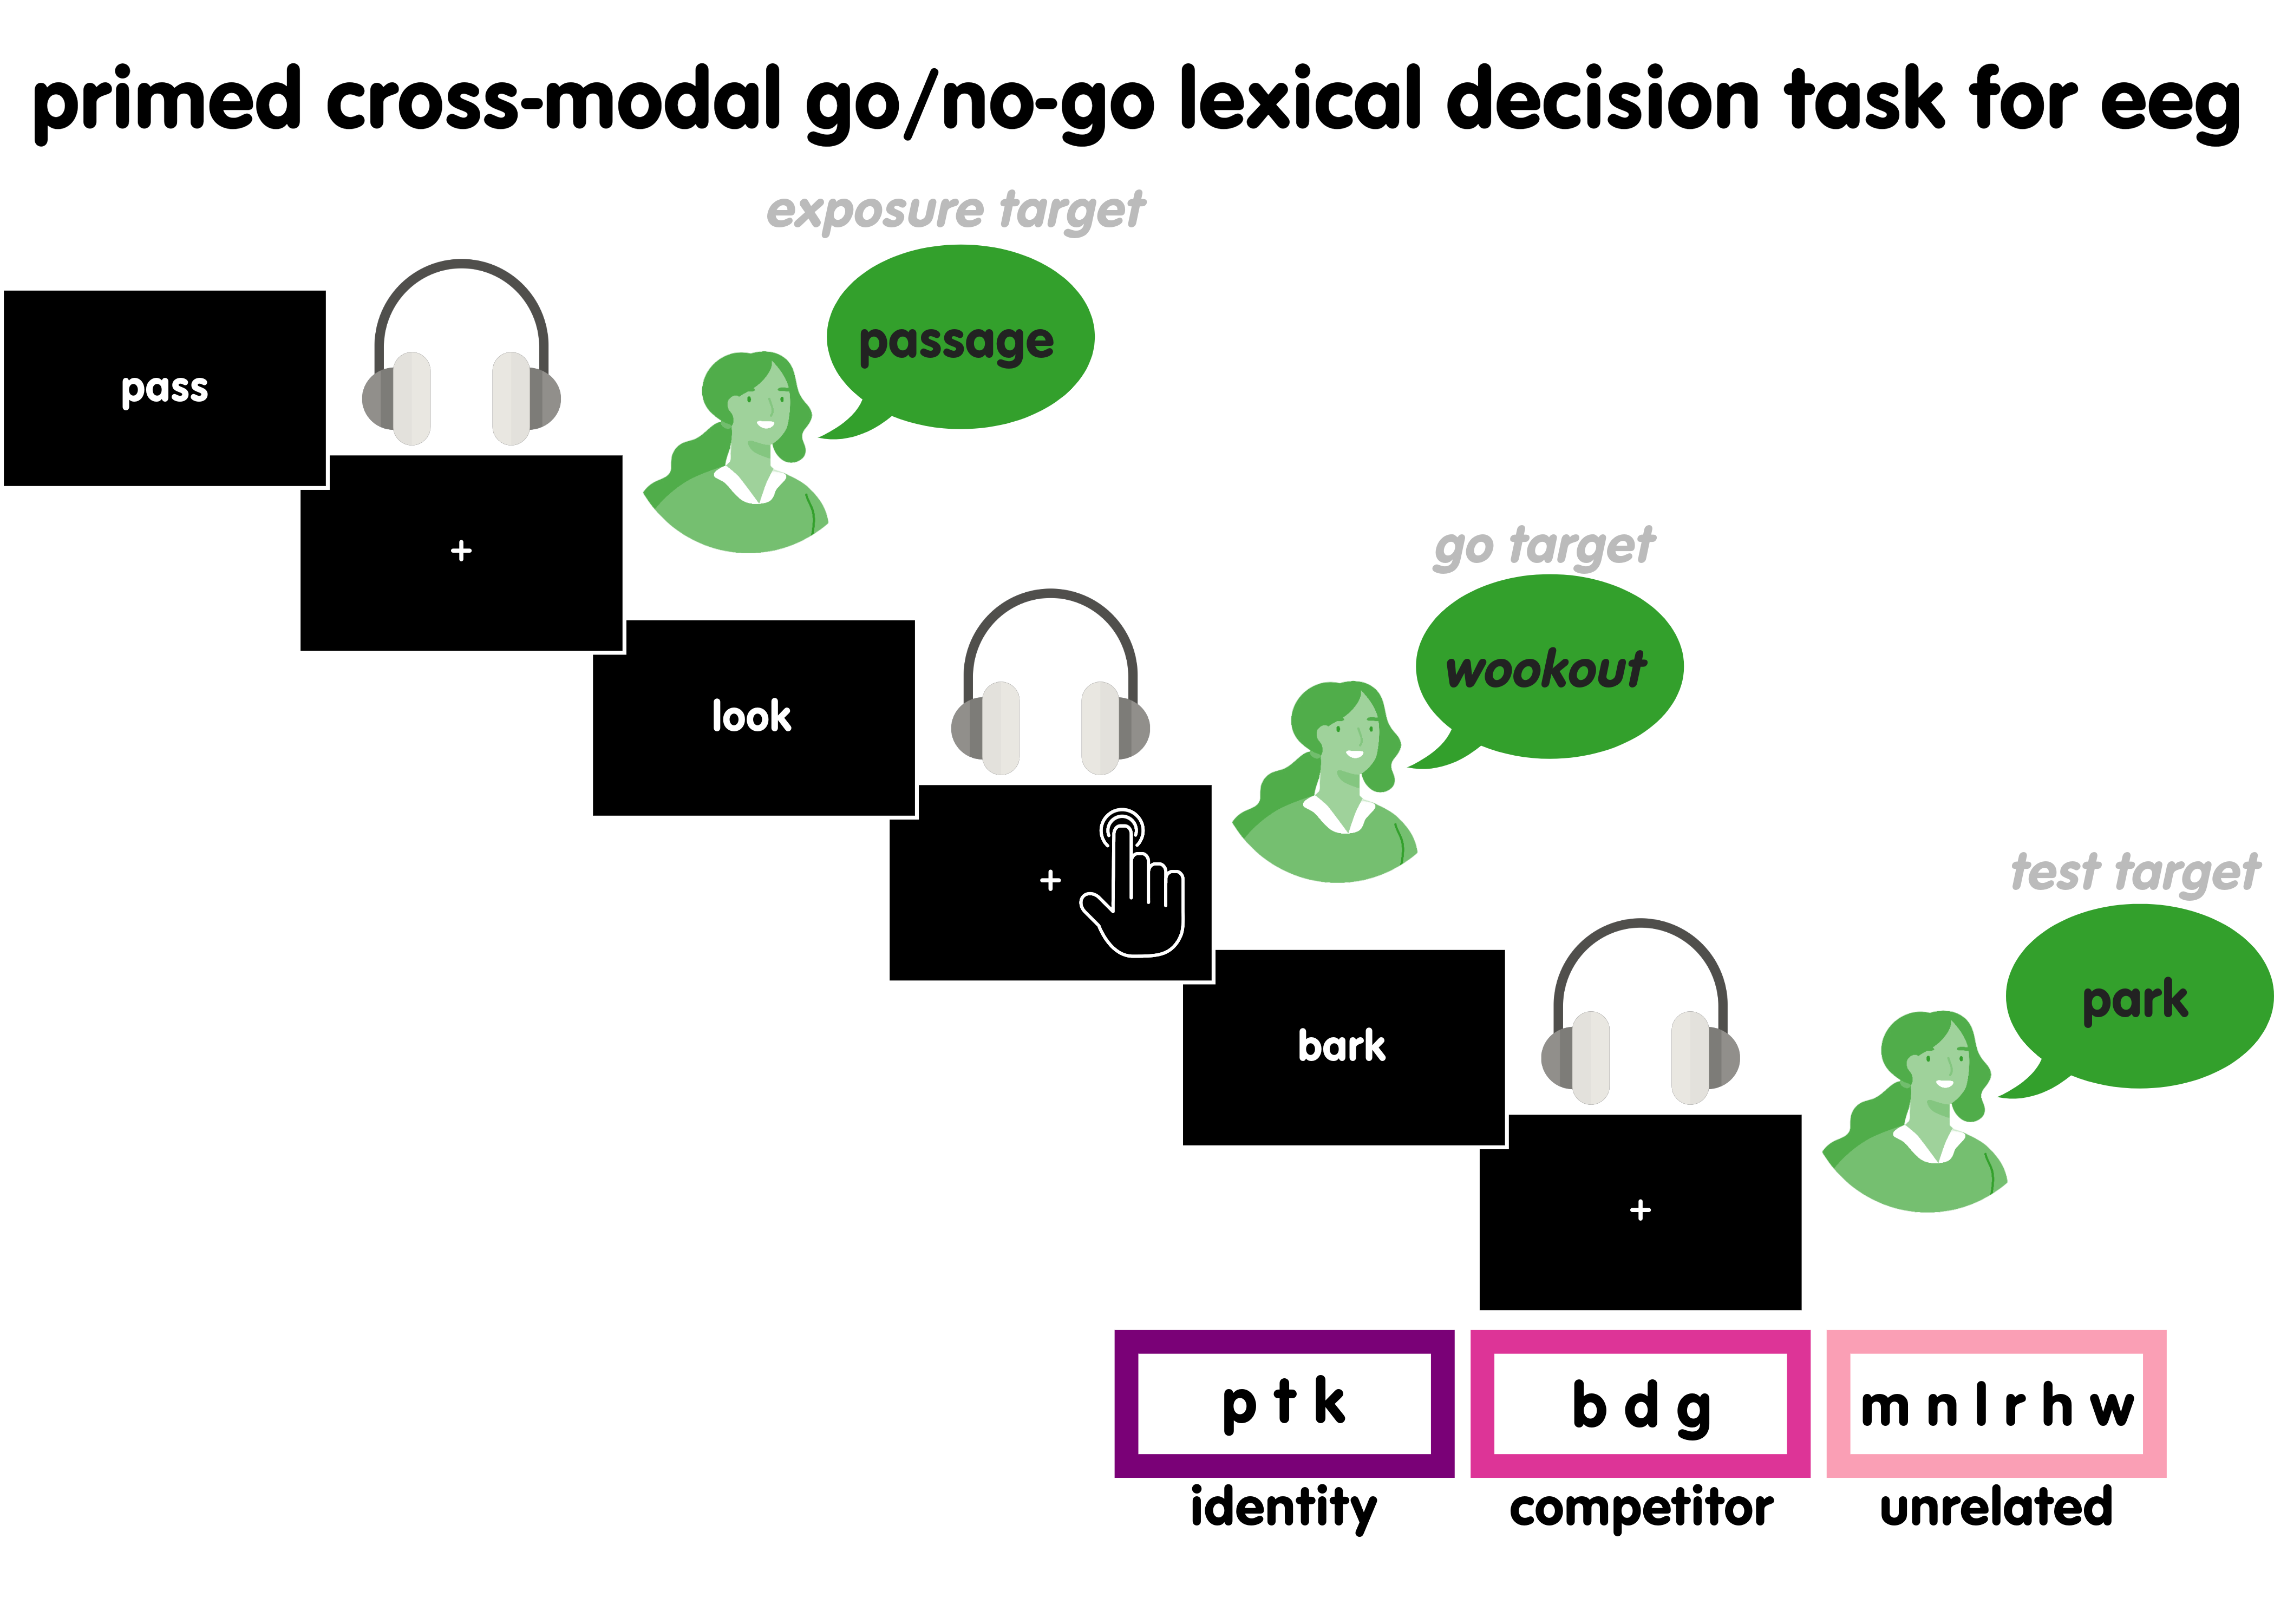
\includegraphics[width=\textwidth]{figures/diss_eeg} 

}

\caption{Experimental design.}\label{fig:study2-fig}
\end{figure}

Analysis of the neurocognitive responses to test targets with respect to prime type (ERP analysis) is described in Section \ref{methods-erp}.
Analysis of the behavioral responses is described in Section \ref{methods-off}.

\hypertarget{behavioral-tasks}{%
\paragraph{Behavioral tasks}\label{behavioral-tasks}}

To measure receptive vocabulary, we administered the English LexTALE (Lemhöfer \& Broersma, 2012).
We used an online implementation of the task, the source code for which can be found at \href{https://github.com/gasparl/lextale}{this GitHub link} (Lukács et al., 2023).
On each trial, participants indicated whether a visual stimulus is a real English word or not by pressing the \emph{yes} or \emph{no} button on the screen.
There were three practice trials and 60 main trials.
One third (20) of the trials were real words.
Receptive vocabulary was calculated as the weighted average of real word and pseudoword accuracy.

To measure inhibitory control, we administered the AX Continuous Performance Task (AX-CPT) (Morales et al., 2015).
The task was programmed with E-Prime 3.0 software (Psychology Software Tools, Pittsburgh, PA).
Each trial had five items in the following order: one cue, three distractors, and one probe.
Participants pressed one of two keys on the keyboard as each item appeared on the screen: one key was the ``no'' key and the other was the ``yes'' key.
Cues and distractors always required a ``no'' response, while the response to the probe depended on the cue.
There were two cue types (A or any other letter) and two probe types (X or any other letter), which together yield four conditions: AX (A cue with X probe; 70\%), AY (A cue with non-X probe; 10\%), BX (non-A cue with X probe; 10\%), and BY (non-A cue with non-X probe; 10\%).
On AX trials, the probe required a ``yes'' response; otherwise, it required a ``no'' response.
AY trials required participants to engage proactive inhibitory control (IC) to inhibit a ``yes'' response following an A cue, while BX trials required participants to engage reactive IC to inhibit a ``yes'' response to an X probe.
There were ten practice trials and 100 main trials in the task.
The mapping of the ``yes'' response to the \emph{d} or \emph{k} key on the keyboard was counterbalanced across participants.
Proactive IC was calculated as the ratio of AY to AX mean probe RTs, and reactive IC was calculated as the ratio of BX to BY mean probe RTs.
In both cases, only trials with correct responses to both the cue and probe were included.
In addition, only probe RTs greater than 200 ms, less than 3000 ms, or within 2.5 standard deviations of each participant's overall mean were included.

\hypertarget{methods-quest}{%
\paragraph{Questionnaires}\label{methods-quest}}

The background questionnaire included the following sets of items: handedness, health history, language history, and demographic information.
The questionnaire was created and administered online via Qualtrics.
The 10-point version of the Edinburgh Handedness Inventory was used to confirm that participants were right-handed (Oldfield, 1971).
Participants also indicated whether they had any blood relatives who were left-handed.
For health history, participants confirmed again that they had normal or corrected-to-normal vision, normal hearing, no history traumatic head injuries, and no history of learning, attention, or language disorders.
Affirmative responses to the latter two items prompted participants to provide additional information about the incident or disorder.
For language history, participants were asked whether they grew up speaking English at home, and if so, whether there were other languages spoken at home.
Participants also selected the label that best described the variety of English they grew up speaking from the following options: American, Australian, British, Canadian, Caribbean, Indian, Irish, Singaporean, or Other (with space to provide a label).
These labels are a subset of ``inner'' and ``outer'' circle World English varieties that were likely to appear in our participant sample (Kang et al., 2024).
Next, participants selected their two main caregivers from a list of family relations.
They also indicated whether both, one, or neither of their two caregivers grew up speaking English at home.
Caregiver variety was coded for the correlation analyses as -1/2, 0, and 1/2, respectively (see Section \ref{methods-corr-erp}).
At the end of the questionnaire, participants provided their age, gender identity, and racial and ethnic background.

The post-experiment questionnaire included two sets of items: the first related to the talker and the second included questions about the participant's own language background.
The questionnaire was created and administered online via Pavlovia's survey platform.
The following items and coding schemes from Study 1 were included: Accent strength, Accent: L2, Comprehensibility, Ease, L1 fluency, L1: Spanish, L2 fluency, L2: English, and Country: Mexico.
Participants were also asked about their own accent and accent strength, L1 and L2, and place of origin as in Study 1.
Ratings were collected on five-point Likert scales anchored at the endpoints with labels containing the modifier ``very'' and a relevant adjective (e.g., ``very weak'' and ``very strong'' for accent strength).
Items requiring categorical responses were collected by presenting a relevant set of options to choose from.

The debriefing questionnaire included 36 items related to language attitudes.
The questionnaire was created and administered online via Pavlovia's survey platform.
There were four main categories: multilingualism, accented speech, grammatical ``correctness,'' and language use in the US/``America.''
Each category had four sub-categories.
For example, the accented speech category had a sub-category probing the relation between fluency and accentedness.
Each sub-category had a negative and a positive item associated with it.
For example, the fluency and accentedness sub-category had the negative item ``Being fluent in English means sounding like a native speaker'' and the positive item ``It's possible to speak English fluently and have a foreign accent at the same time.''
This resulted in 32 items.
There were four additional miscellaneous items that did not have obvious pairings.
Responses were provided on a five-point scale anchored at the endpoints with the labels ``strongly disagree'' (1) and ``strongly agree'' (5).
The 16 negative items were reverse-coded before all 36 items were averaged into a mean language attitude score.
After the language attitudes questions, participants were asked to provide feedback about their experience in the study.
In addition, they were able to provide their email address if they wanted to know the results of the study.

\hypertarget{procedure}{%
\subsubsection{Procedure}\label{procedure}}

When a participant arrived for their testing session, the researcher confirmed their eligibility, showed the participant the EEG equipment and materials, and explained the testing procedure.
The participant then provided written informed consent and completed the background questionnaire, followed by the LexTALE.
Next, the participant completed the LDT while EEG was recorded.
The EEG task lasted between 30 and 40 minutes, including breaks between each of the six blocks, and was immediately followed by the post-experiment questionnaire.
Participants then completed the AX-CPT, followed by the debriefing questionnaire.
At the end of the session, the participant received compensation.

\hypertarget{methods-eeg}{%
\paragraph{EEG acquisition and pre-processing}\label{methods-eeg}}

Scalp EEG was recorded at a continuous sampling rate of 500 Hz from 32 active Ag/AgCl electrodes (Brain Products ActiCap, Germany).
Electrodes were mounted in an elastic cap according to the extended 10-20 system (Chatrian et al., 1985), with the exception of CP5 and CP6.
Instead, these were placed at the outer canthus of the left eye (HEOG) and above the left eyebrow (VEOG), respectively, to monitor for ocular artifacts.
The left mastoid was used as the online reference.
The EEG signal was amplified with a mobile BrainVision ActiCHamp system and filtered with a 0.05--100 Hz bandpass filter.
Impedances were kept below 15 k\(\Omega\).

Offline data pre-processing was conducted with the EEGLAB MATLAB toolbox (Delorme \& Makeig, 2004).
EEG data were filtered with a 30 Hz low-pass filter (24 dB/octave roll-off) and re-referenced to the average of the two mastoids.
To prepare the data for Independent Component Analysis (ICA), we first removed recordings taken between each block and before/after the experiment.
We then conducted manual artifact rejection to remove atypical eye/muscle activity and periods of line/channel noise.
Next, we identified and removed bad head channels (not eye electrodes), which either exceeded a maximum flatline duration of five seconds, exhibited a channel correlation of lower than 0.6, or exceeded the line noise threshold of four standard deviations.
The data were then submitted to ICA.
We took a data-driven approach to identifying artifactual ICA components.
Across participants, we first determined the 0.9 quantile for the component probabilities within each category of non-brain activity: muscle, eye, heart, line noise, channel noise, and other.
Components that exceeded these thresholds were then removed.
After removing artifactual ICA components, any head channels that had previously been removed were interpolated.

The EEG signal was time-locked to the onset of the auditory target and epochs were baseline-corrected relative to a 200 ms pre-stimulus interval.
Finally, epochs with peak-to-peak activity exceeding a 60 \(\mu\)V threshold in eye channels or with activity above/below a 100 \(\mu\)V threshold in head channels were rejected.
Across all participants, 29 of test trials were removed due to excessive artifacts, leaving an average of 215 test trials per participant out of 216.
The data for each channel of interest (19) and test trial (216) was then extracted in 2 ms increments from -200 to 800 ms relative to the onset of the auditory target for analysis and visualization.
The channels of interest were in frontal (F7, F3, Fz, F4, F8), fronto-central (FC5, FC1, FC2, FC6), central/centro-parietal (C3, Cz, C4, CP1, CP2), and parietal (P7, P3, Pz, P4, P8) regions based on previous research (Kapnoula \& McMurray, 2021; Sarrett et al., 2020; Toscano et al., 2010).

\hypertarget{methods-erp}{%
\paragraph{ERP data analyses}\label{methods-erp}}

Data analysis and visualization were conducted in R version 4.2.2 (R Core Team, 2022).
Only accurate test trials were included in the ERP analyses.
Across all participants, we removed 7.04\% of the test trials that remained after EEG pre-processing, leaving an average of 200 test trials per participant out of 216 for analysis.
By condition, there were an average of 69 Identity test trials, 67 Competitor test trials, and 64 Unrelated test trials per participant included in the analyses.

We analyzed the data in three time windows: 175-250 ms (N1), 250-375 (P2), and 450-650 (N400).
These specific time ranges were chosen based on Sarrett et al. (2020) and visual inspection of the average waveforms across all channels, trials, and conditions (i.e., independent of the critical manipulations).
Of the 19 channels of interest, we followed the procedure outlined in Kapnoula and McMurray (2021) to select the channels for each time window (again, independent of the critical manipulations).
Channels with an average amplitude across conditions of less than -1 \(\mu\)V in the N1 and N400 time windows were included in each analysis.
Channels with an average amplitude across conditions of greater than +1 \(\mu\)V in the P2 time window were included.
The N400 analysis ultimately included all 19 channels.
For the N1 analysis, all but two channels (F7 and F8) were included.
For the P2 analysis, 10 frontal (F7, F3, Fz, F4, F8) and fronto-central (FC5, FC1, FC2, FC6, Cz) channels were included.
Finally, within each time window, we averaged the ERPs for each participant and trial by channel.

Three mixed-effects models were fitted to the trial-level ERP data in each time window with the \emph{lme4} package (Bates et al., 2015).
Type-II analysis-of-variance tables were calculated and Wald chi-square tests were conducted with the \emph{car} package (Fox \& Weisberg, 2019).
Estimated marginal means were calculated and pairwise comparisons were conducted with the \emph{emmeans} package (Lenth, 2022).
Pairwise \emph{p}-values were adjusted with the Hommel method to control the family-wise error rate (Blakesley et al., 2009).

Analyses modeled the effects of prime type (Prime), amount of exposure (Exposure), and their interaction on the ERPs in each time window.
The three levels of Prime (Identity, Competitor, Unrelated) were Helmert contrast-coded.
Exposure was defined as the mean-centered number of Exposure targets encountered before the given Test target.
Mean-centered VOT and target frequency were included as covariates.
Random intercepts were included for item, participant, and channel.
Random by-participant slopes for Prime were included during initial model fitting; however, these slopes were removed from all three analyses due to non-convergence.

\hypertarget{methods-off}{%
\paragraph{Offline data analyses}\label{methods-off}}

Analyses were conducted with the same R packages as the ERP analyses.
To establish evidence of perceptual adaptation in behavior, we compared test and filler targets in terms of accuracy (Target type analysis).
Within test targets, we also investigated the effect of prime type on accuracy (Prime type analysis).
We could not analyze RT in either analysis, because only inaccurate trials had responses for these items.

The data were cleaned prior to analysis.
All accurate trials were included.
Inaccurate trials with RTs less than 250 ms were removed (\emph{N} = 9; 0.06\%).
RT was calculated from the onset of the target.
Generalized linear mixed-effects models with a binomial family function were fit to the trial-level data.

The Target type analysis modeled the effects of target type (Target), amount of exposure (Exposure), and their interaction on accuracy (1,0).
The two levels of Target (Test, Filler) were sum contrast-coded.
As in the ERP analyses, Exposure was defined as the mean-centered number of Exposure targets encountered before the given target.
Mean-centered VOT and target frequency were included as covariates.
Random intercepts were included for participant and the interaction between prime and target (to distinguish the three presentations of each test target with a different prime).
Random by-participant slopes were also included for Target.

The Prime type analysis modeled the effects of prime type (Prime), amount of exposure (Exposure), and their interaction on test target accuracy (1,0).
Prime and Exposure were specified the same way as in the ERP analyses.
Random intercepts were included for participant and target, with by-participant random slopes for Prime.

\hypertarget{methods-corr-erp}{%
\paragraph{Correlation analysis}\label{methods-corr-erp}}

Pairwise correlations were calculated with the \emph{psych} R package (Revelle, 2023).
From the AX-CPT, we included both Proactive and Reactive IC.
We also included LexTALE scores (Vocabulary) and language attitude scores (Attitudes).
From the background questionnaire, we included ``Caregiver variety'' as a measure of previous exposure to L2-accented speech (see Section \ref{methods-quest}).
We also included the measures from the post-experiment questionnaire: Accent strength, Accent: L2, Comprehensibility, Ease, L1 fluency, L1: Spanish, L2 fluency, L2: English, and Country: Mexico.

To capture performance on the EEG task, we calculated the magnitude of the priming effects on four measures: Test target accuracy, N1 amplitude, P2 amplitude, and N400 amplitude.
The responses to Identity, Competitor, and Unrelated primes were averaged, and then the mean of the averaged Competitor and Unrelated responses was subtracted from the averaged Identity responses.
For the ERP calculations, we took the absolute value of these differences.

\hypertarget{results-4}{%
\subsection{Results}\label{results-4}}

\hypertarget{behavioral-results}{%
\subsubsection{Behavioral results}\label{behavioral-results}}

\hypertarget{target-type-analysis}{%
\paragraph{Target type analysis}\label{target-type-analysis}}

We observed a significant interaction between Target and Exposure (\(\chi^2\)(1, \emph{N} = 2) = 10.78, \emph{p} = .001), as well as main effects of Target (\(\chi^2\)(1, \emph{N} = 2) = 4.42, \emph{p} = .036) and Exposure (\(\chi^2\)(1, \emph{N} = 2) = 79.76, \emph{p} \textless{} .001).
The rate of improvement on Test targets (\emph{M} = 0.021, 95\% CI {[}0.016, 0.025{]}) was greater than that on Filler targets (\emph{M} = 0.010, 95\% CI {[}0.005, 0.014{]}; \emph{z} = 3.28, \emph{p} = .001).

This difference in adaptation between target types is illustrated by comparing the estimated marginal mean accuracy at the beginning of the task (Exposure = -36) to that at the end (Exposure = 36).
Accuracy on Filler targets started at 0.91 (95\% CI {[}0.87, 0.94{]}) and ended at 0.96 (95\% CI {[}0.93, 0.97{]}), while accuracy on Test targets started at 0.93 (95\% CI {[}0.90, 0.95{]}) and ended at 0.98 (95\% CI {[}0.97, 0.99{]}).
Accuracy significantly improved between these two time points for both Filler (\emph{z} = 4.40, \emph{p} \textless{} .001) and Test (\emph{z} = 8.43, \emph{p} \textless{} .001) targets.
However, the enhanced rate of learning for test targets resulted in a significant difference between Filler and Test target accuracy at the end of the task (\emph{z} = 3.37, \emph{p} \textless{} .001) that was not present at the beginning (\emph{z} = 0.76, \emph{p} = .450).
The results are shown in Figure \ref{fig:behave-fig}.

\hypertarget{prime-type-analysis}{%
\paragraph{Prime type analysis}\label{prime-type-analysis}}

We observed significant main effects of Prime (\(\chi^2\)(2, \emph{N} = 3) = 63.65, \emph{p} \textless{} .001) and Exposure (\(\chi^2\)(1, \emph{N} = 2) = 48.95, \emph{p} \textless{} .001).
The interaction between the two factors was not significant (\(\chi^2\)(2, \emph{N} = 3) = 0.66, \emph{p} = .720).
Overall, accuracy increased with exposure regardless of prime type (\(\beta\) = 0.021).
Within prime type, accuracy increased linearly from Unrelated (\emph{M} = 0.95, 95\% CI {[}0.92, 0.96{]}) to Competitor (\emph{M} = 0.97, 95\% CI {[}0.96, 0.98{]}) to Identity (\emph{M} = 0.99, 95\% CI {[}0.98, 0.99{]}) targets.
Accuracy was significantly different among the different levels of Prime: Identity versus Competitor (\emph{z} = 4.24, \emph{p} \textless{} .001), Identity versus Unrelated (\emph{z} = 7.86, \emph{p} \textless{} .001), and Competitor versus Unrelated (\emph{z} = 4.32, \emph{p} \textless{} .001).
The results are shown in Figure \ref{fig:test-fig}.

\hypertarget{summary}{%
\paragraph{Summary}\label{summary}}

The behavioral data provide strong evidence for talker-specific adaptation to Spanish-accented voiceless stops.
We first compared accuracy on test targets, with voiceless stop onsets that were perceptually confusible with voiced stops (e.g., \emph{park}-\emph{bark}), to accuracy on filler targets (e.g., \emph{rhubarb}).
Exposure was operationalized as the (mean-centered) number of exposure targets (e.g., \emph{passage}) that the participant had heard before encountering a given target.
Participants adapted to both the talker and task, exhibiting improved accuracy on both types of targets; however, improvements in word recognition were strongest for the test targets.
This enhanced performance on test targets suggests that exposure to disambiguating lexical contexts for Spanish-accented /p/, /t/, and /k/ improved perception in ambiguous lexical contexts.

\begin{figure}[H]

{\centering 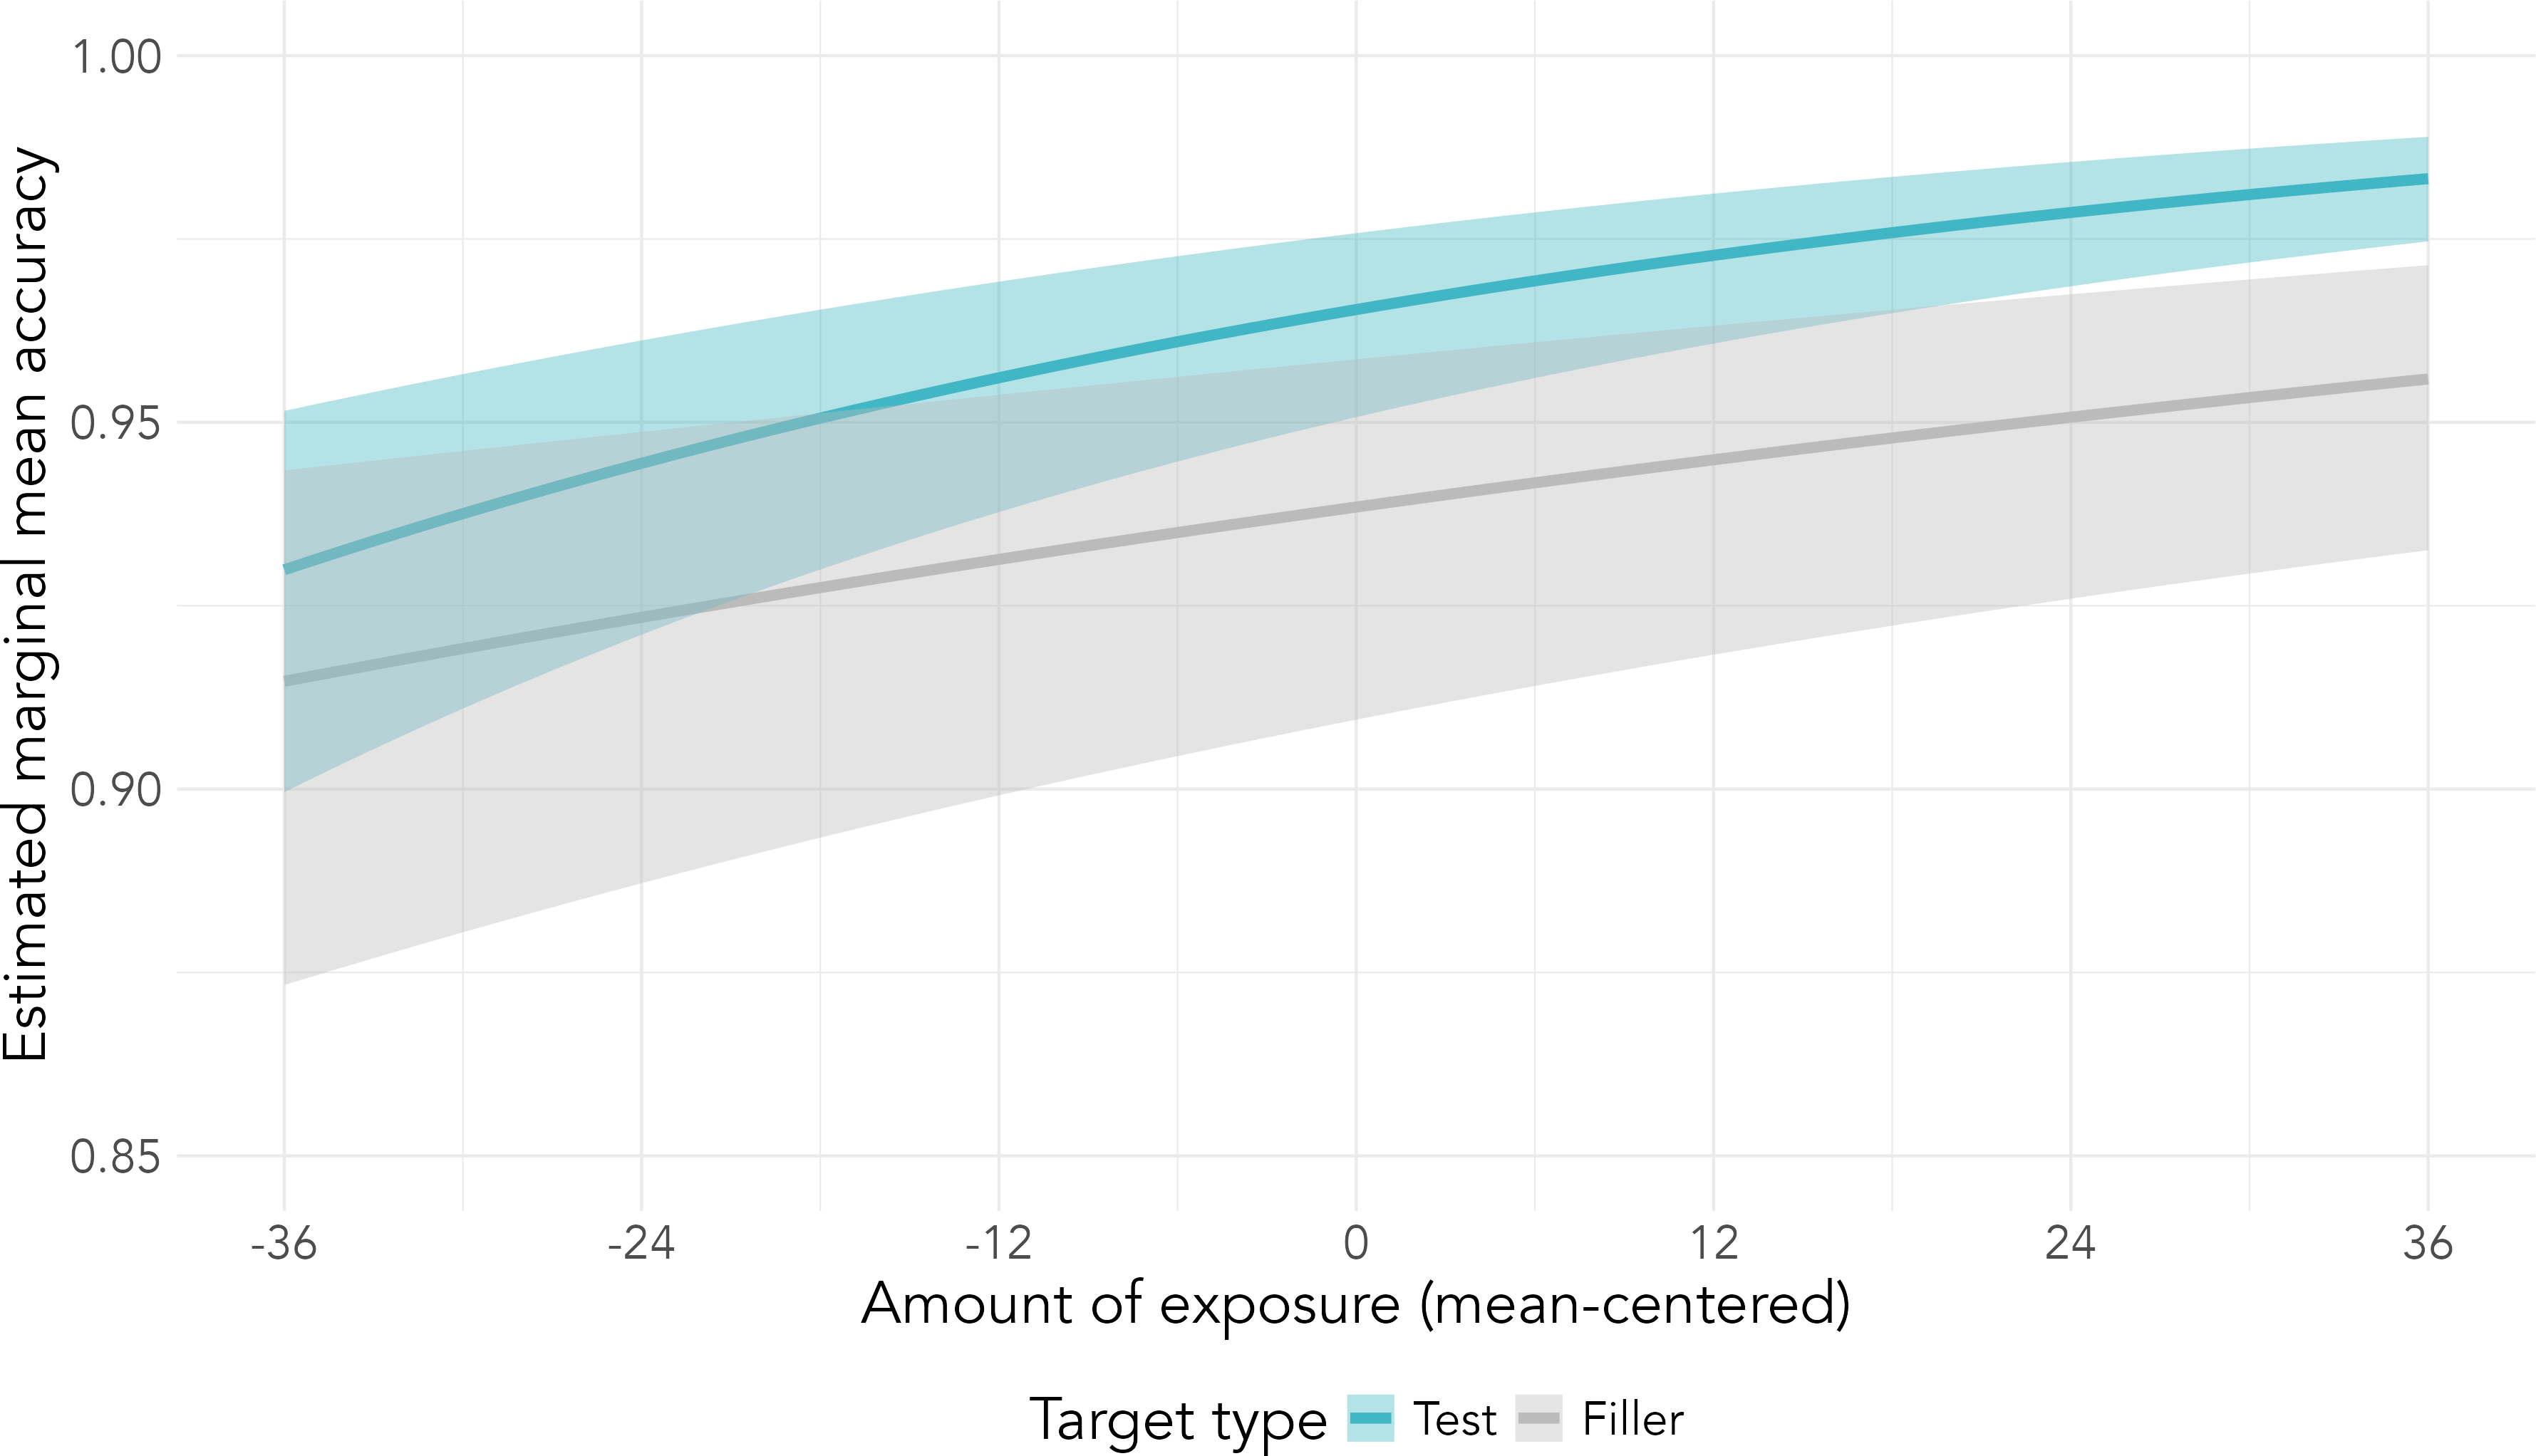
\includegraphics[width=\textwidth]{sections/code/outputs/behave_plot} 

}

\caption{Test target accuracy by Target type and Exposure.}\label{fig:behave-fig}
\end{figure}

We then compared accuracy on test targets for each type of prime: Identity, Competitor, and Unrelated.
While overall accuracy increased with exposure, as demonstrated in the previous analysis, priming effects remained stable.
These priming effects were in the expected direction, with Identity primes yielding the highest accuracy on Test targets, followed by Competitor primes, then Unrelated primes.

\begin{figure}[H]

{\centering 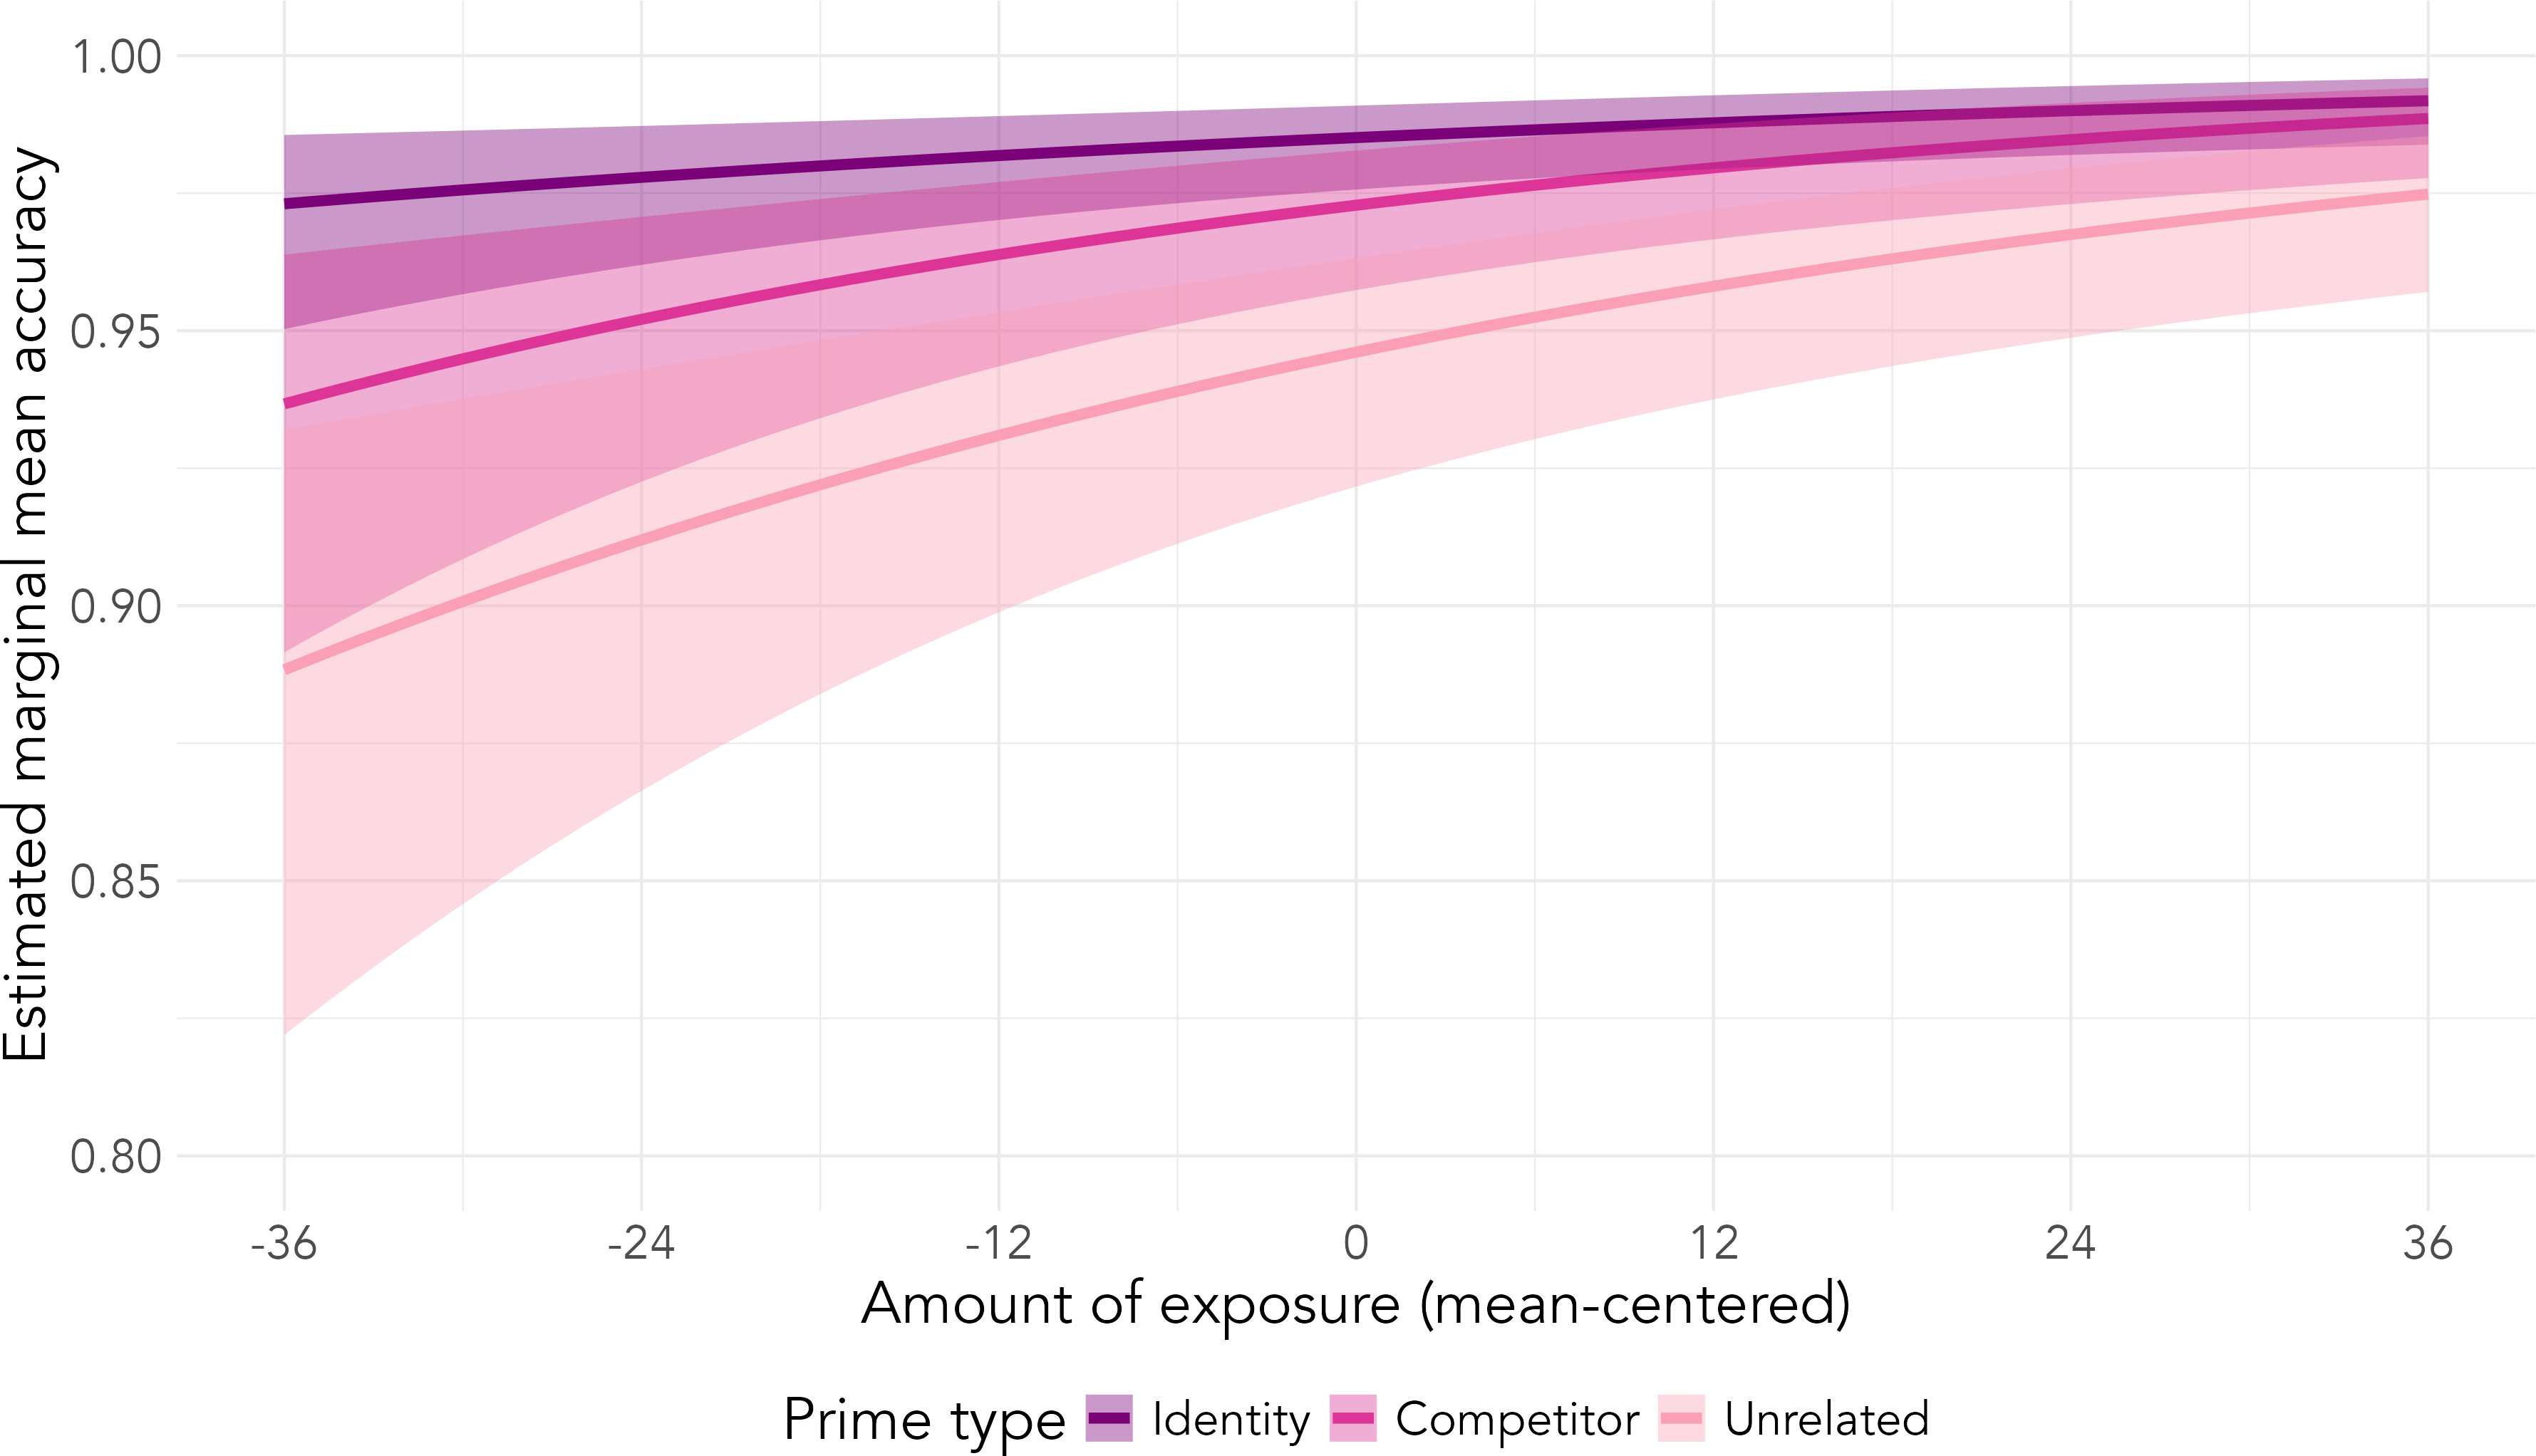
\includegraphics[width=\textwidth]{sections/code/outputs/test_plot} 

}

\caption{Test target accuracy by Prime type and Exposure.}\label{fig:test-fig}
\end{figure}

\hypertarget{erp-results}{%
\subsubsection{ERP results}\label{erp-results}}

Grand mean waveforms, averaging across participants (40), amount of exposure (72), and channels (17 from the N1 analysis) are shown in Figure \ref{fig:grand-fig}.

\begin{figure}[H]

{\centering 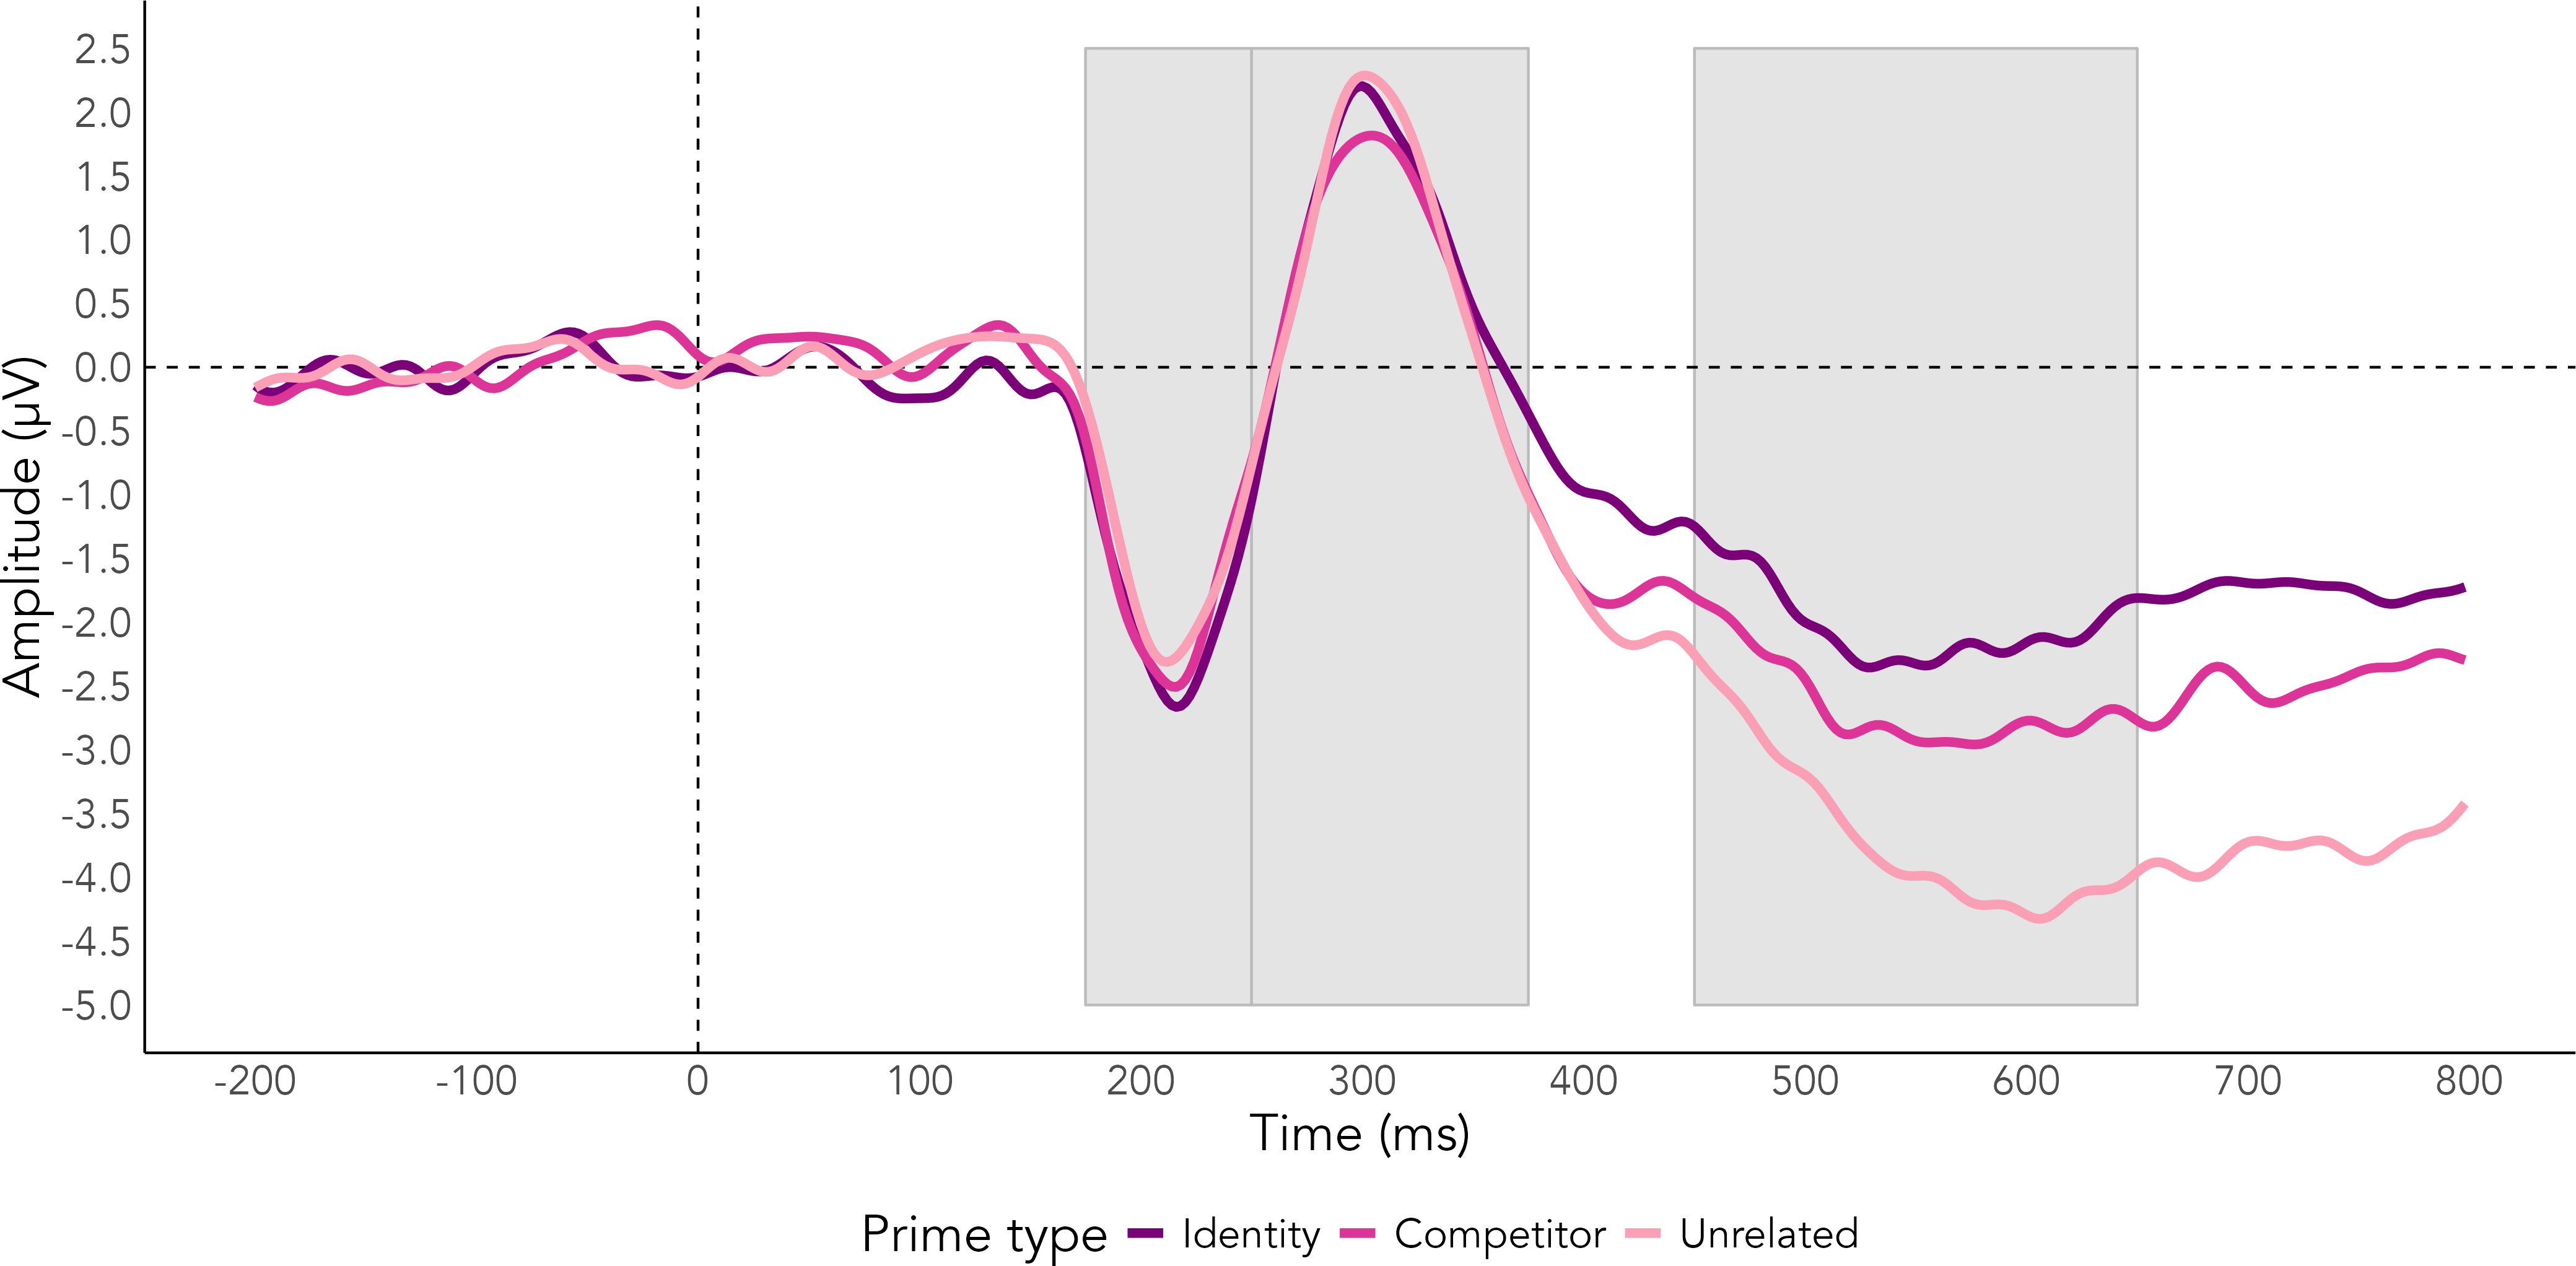
\includegraphics[width=\textwidth]{sections/code/outputs/grand_plot} 

}

\caption{Grand mean waveforms by Prime type.}\label{fig:grand-fig}
\end{figure}

\hypertarget{ms}{%
\paragraph{175-250 ms}\label{ms}}

We observed a significant interaction between Prime and Exposure (\(\chi^2\)(2, \emph{N} = 3) = 56.25, \emph{p} \textless{} .001), as well as main effects of Prime (\(\chi^2\)(2, \emph{N} = 3) = 39.45, \emph{p} \textless{} .001) and Exposure (\(\chi^2\)(1, \emph{N} = 2) = 55.05, \emph{p} \textless{} .001).
Specifically, we observed an increase in N1 amplitude following Identity primes (\emph{M} = -0.002, 95\% CI {[}-0.006, 0.002{]}) that contrasted with a decrease in amplitude following Competitor primes (\emph{M} = 0.005, 95\% CI {[}0.001, 0.009{]}) and Unrelated primes (\emph{M} = 0.021, 95\% CI {[}0.017, 0.025{]}).
Pairwise comparisons as a function of Exposure revealed significant differences among all three types of primes: Identity versus Competitor (\emph{z} = 2.28, \emph{p} = .023), Identity versus Unrelated (\emph{z} = 7.31, \emph{p} \textless{} .001), and Competitor versus Unrelated (\emph{z} = 5.10, \emph{p} \textless{} .001).

To contextualize the interaction, we report differences in Prime at the lowest (-36) and highest (36) amounts of Exposure (see Figure \ref{fig:erp-eff-fig}, N1).
At the beginning of the task, the N1 was largest for Test targets following Unrelated primes (\emph{M} = -2.41, 95\% CI {[}-2.98, -1.84{]}), with successively smaller amplitudes for Competitor primes (\emph{M} = -1.94, 95\% CI {[}-2.50, -1.38{]}) and Identity primes (\emph{M} = -1.86, 95\% CI {[}-2.42, -1.29{]}).
Pairwise comparisons showed significant differences in amplitude for Identity versus Unrelated (\emph{z} = 4.40, \emph{p} \textless{} .001) and Competitor versus Unrelated (\emph{z} = 3.89, \emph{p} \textless{} .001); however, the difference in amplitude for Identity versus Competitor (\emph{z} = 0.70, \emph{p} = .482) was not significant.
By the end of the task, this order had reversed from Identity primes (\emph{M} = -2.00, 95\% CI {[}-2.57, -1.44{]}) to Competitor primes (\emph{M} = -1.57, 95\% CI {[}-2.14, -1.00{]}) to Unrelated primes (\emph{M} = -0.89, 95\% CI {[}-1.46, -0.33{]}).
These amplitudes were all significantly different from one another: Identity versus Competitor (\emph{z} = 3.41, \emph{p} \textless{} .001), Identity versus Unrelated (\emph{z} = 9.18, \emph{p} \textless{} .001), and Competitor versus Unrelated (\emph{z} = 5.43, \emph{p} \textless{} .001).
However, within each prime type, the change in amplitude was not significant for the Identity condition (\emph{z} = 1.02, \emph{p} = .307).
By contrast, Competitor priming (\emph{z} = 2.45, \emph{p} = .014) and Unrelated priming (\emph{z} = 9.89, \emph{p} \textless{} .001) increased significantly from the beginning to the end of the task.

\hypertarget{ms-1}{%
\paragraph{250-375 ms}\label{ms-1}}

As in the previous time window, we observed a significant interaction between Prime and Exposure (\(\chi^2\)(2, \emph{N} = 3) = 27.13, \emph{p} \textless{} .001).
We also observed a main effect of Prime (\(\chi^2\)(2, \emph{N} = 3) = 8.48, \emph{p} = .014).
The interaction was driven by an increase in P2 amplitude following Unrelated primes (\emph{M} = 0.010, 95\% CI {[}0.005, 0.016{]}) in contrast with a decrease following Identity primes (\emph{M} = -0.012, 95\% CI {[}-0.017, -0.007{]}) and Competitor primes (\emph{M} = -0.002, 95\% CI {[}-0.007, 0.004{]}).
Pairwise comparisons as a function of Exposure revealed significant differences among all three types of primes: Identity versus Competitor (\emph{z} = 6.15, \emph{p} \textless{} .001), Identity versus Unrelated (\emph{z} = 13.03, \emph{p} \textless{} .001), and Competitor versus Unrelated (\emph{z} = 6.99, \emph{p} \textless{} .001).

To investigate the differences in priming across the task, we conducted pairwise comparisons of the effects at the beginning and end of the task (see Figure \ref{fig:erp-eff-fig}, P2).
During the initial stages of adaptation, Identity primes elicited larger P2 effects on Test targets (\emph{M} = 2.08, 95\% CI {[}1.41, 2.74{]}) than Competitor primes (\emph{M} = 1.57, 95\% CI {[}0.91, 2.24{]}; \emph{z} = 3.09, \emph{p} = .004) or Unrelated primes (\emph{M} = 1.32, 95\% CI {[}0.65, 1.99{]}; \emph{z} = 4.40, \emph{p} \textless{} .001).
Competitor and Unrelated primes did not differ from one another (\emph{z} = 1.55, \emph{p} = .120).
In the later stages of adaptation, Identity primes (\emph{M} = 1.20, 95\% CI {[}0.54, 1.86{]}) elicited similar effects to Competitor primes (\emph{M} = 1.46, 95\% CI {[}0.79, 2.13{]}; \emph{z} = 1.48, \emph{p} = .138).
At the same time, Unrelated primes (\emph{M} = 2.05, 95\% CI {[}1.39, 2.72{]}) diverged from competitor primes (\emph{z} = 3.53, \emph{p} \textless{} .001).
Identity and Unrelated primes remained different from one another (\emph{z} = 5.19, \emph{p} \textless{} .001), though in the opposite direction.
Overall, the effects of Competitor primes remained stable in this time window (\emph{z} = 0.57, \emph{p} = .566), while those of Identity primes (\emph{z} = 4.47, \emph{p} \textless{} .001) and Unrelated primes (\emph{z} = 3.53, \emph{p} \textless{} .001) reversed.

\hypertarget{ms-2}{%
\paragraph{450-650 ms}\label{ms-2}}

We observed a significant interaction between Prime and Exposure (\(\chi^2\)(2, \emph{N} = 3) = 170.18, \emph{p} \textless{} .001), a main effect of Prime (\(\chi^2\)(2, \emph{N} = 3) = 910.70, \emph{p} \textless{} .001), and a main effect of Exposure (\(\chi^2\)(1, \emph{N} = 2) = 6.52, \emph{p} = .011).
As in the N1 time window, the interaction was driven by an increase in amplitude following Identity primes (\emph{M} = -0.018, 95\% CI {[}-0.022, -0.013{]}) coupled with a decrease in amplitude following Competitor primes (\emph{M} = 0.003, 95\% CI {[}-0.001, 0.008{]}) and Unrelated primes (\emph{M} = 0.026, 95\% CI {[}0.022, 0.031{]}).
These slopes were significantly different from one another: Identity versus Competitor (\emph{z} = 6.15, \emph{p} \textless{} .001), Identity versus Unrelated (\emph{z} = 13.03, \emph{p} \textless{} .001), and Competitor versus Unrelated (\emph{z} = 6.99, \emph{p} \textless{} .001).

We observed a typical N400 effect at the beginning of the experiment, with amplitudes increasing from Identity (\emph{M} = -1.35, 95\% CI {[}-2.07, -0.64{]}) to Competitor (\emph{M} = -2.64, 95\% CI {[}-3.36, -1.93{]}) to Unrelated (\emph{M} = -4.53, 95\% CI {[}-5.25, -3.81{]}) primes (see Figure \ref{fig:erp-eff-fig}, N400).
These effects were all significantly different from one another: Identity versus Competitor (\emph{z} = 10.09, \emph{p} \textless{} .001), Identity versus Unrelated (\emph{z} = 23.45, \emph{p} \textless{} .001), and Competitor versus Unrelated (\emph{z} = 14.53, \emph{p} \textless{} .001).
By the end of the experiment, these effects had converged, with Identity (\emph{M} = -2.62, 95\% CI {[}-3.33, -1.90{]}), Competitor (\emph{M} = -2.42, 95\% CI {[}-3.14, -1.70{]}), and Unrelated (\emph{M} = -2.62, 95\% CI {[}-3.34, -1.91{]}) primes eliciting similar N400 effects: Identity versus Competitor (\emph{z} = 1.48, \emph{p} = .280), Identity versus Unrelated (\emph{z} = 0.05, \emph{p} = .963), and Competitor versus Unrelated (\emph{z} = 1.55, \emph{p} = .242).
This convergence in priming effects was driven by significant changes in Identity priming (\emph{z} = 8.22, \emph{p} \textless{} .001) and Unrelated priming (\emph{z} = 11.63, \emph{p} \textless{} .001), while Competitor priming remained the same (\emph{z} = 1.39, \emph{p} = .164).

\hypertarget{summary-1}{%
\paragraph{Summary}\label{summary-1}}

The results of the ERP analyses revealed a shift from lexico-semantic to acoustic processing over time.
These changes are illustrated in Figure \ref{fig:erp-eff-fig}.

\begin{figure}[H]

{\centering 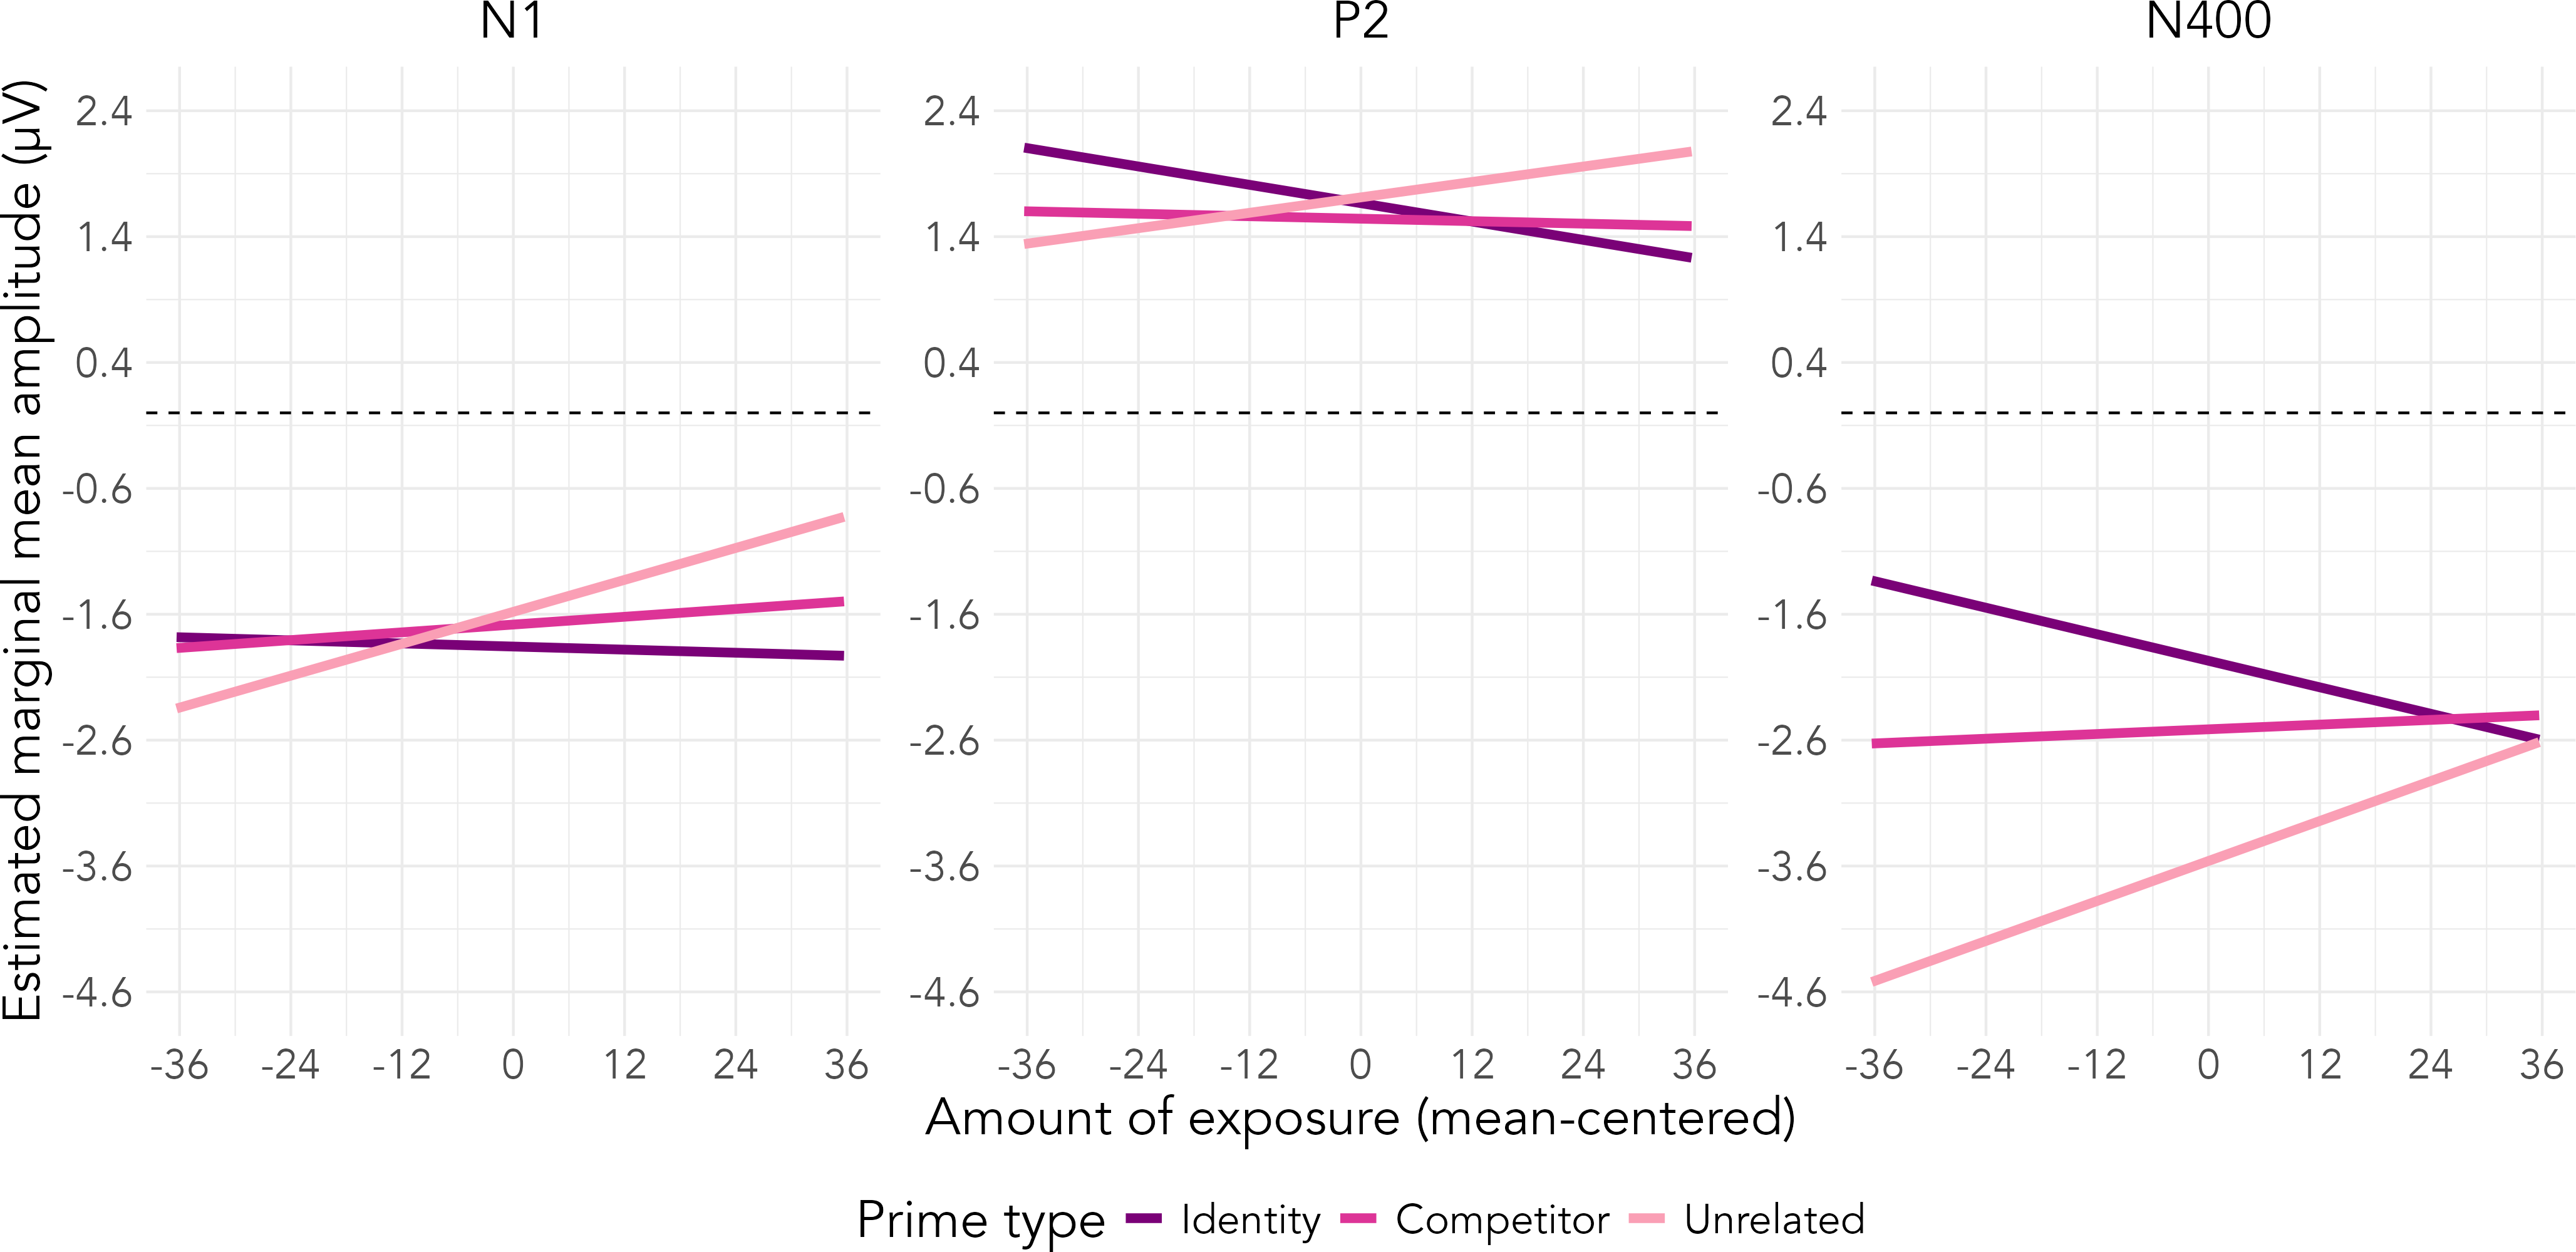
\includegraphics[width=\textwidth]{sections/code/outputs/erp_eff} 

}

\caption{Estimated marginal mean amplitudes by Prime and Exposure on the N1, P2, and N400.}\label{fig:erp-eff-fig}
\end{figure}

Between 175 and 250 ms, the amplitude of the neurocognitive responses to Competitor and Unrelated primes decreased in negativity with increasing exposure.
The N1 component in this time window is sensitive to the perception of voicing contrasts, with voiced stops eliciting larger (more negative) amplitudes than voiceless stops (Getz \& Toscano, 2021).
At the beginning of the experiment, Identity and Competitor priming effects patterned together (Unrelated \textgreater{} Competitor = Identity).
By the end of the experiment, N1 amplitude exhibited graded sensitivity to prime type (Identity \textgreater{} Competitor \textgreater{} Unrelated).
The decrease in negativity for the two mismatched prime types reflects improvements in perception of the ambiguous test targets.

In the 250-375 ms time window, Unrelated priming effects became more positive, while Identity priming effects became less positive with exposure.
The P2 component elicited in this time window indexes phonetic categorization, with less effortful processing associated with larger (more positive) amplitudes (Crowley \& Colrain, 2004).
P2 amplitude exhibited a reversal in priming effects from the beginning (Identity \textgreater{} Competitor = Unrelated) to the end (Unrelated \textgreater{} Competitor = Identity) of the task.
The increase in positivity for Unrelated prime trials reflects facilitation of categorizing the ambiguous Test targets with increased exposure.

The same differential effects of prime type were observed in the 450-650 ms time window, with Unrelated priming effects becoming less negative and Identity priming effects becoming more negative with exposure.
The N400 component in this time window indexes lexico-semantic access, with more effortful processing associated with larger (more negative) amplitudes (Federmeier, 2021).
Overall, the N400 started with graded sensitivity to prime type (Unrelated \textgreater{} Competitor \textgreater{} Identity) and ended with a lack of sensitivity (Unrelated = Competitor = Identity).
The reduction in the difference between Identity and Unrelated primes suggests that lexico-semantic processing became less sensitive to prime type over time.

\hypertarget{correlation-results}{%
\subsubsection{Correlation results}\label{correlation-results}}

Pairwise correlations are shown in Figure \ref{fig:erp-corr-fig}.
Only items with significant correlations are displayed.

\begin{figure}[H]

{\centering 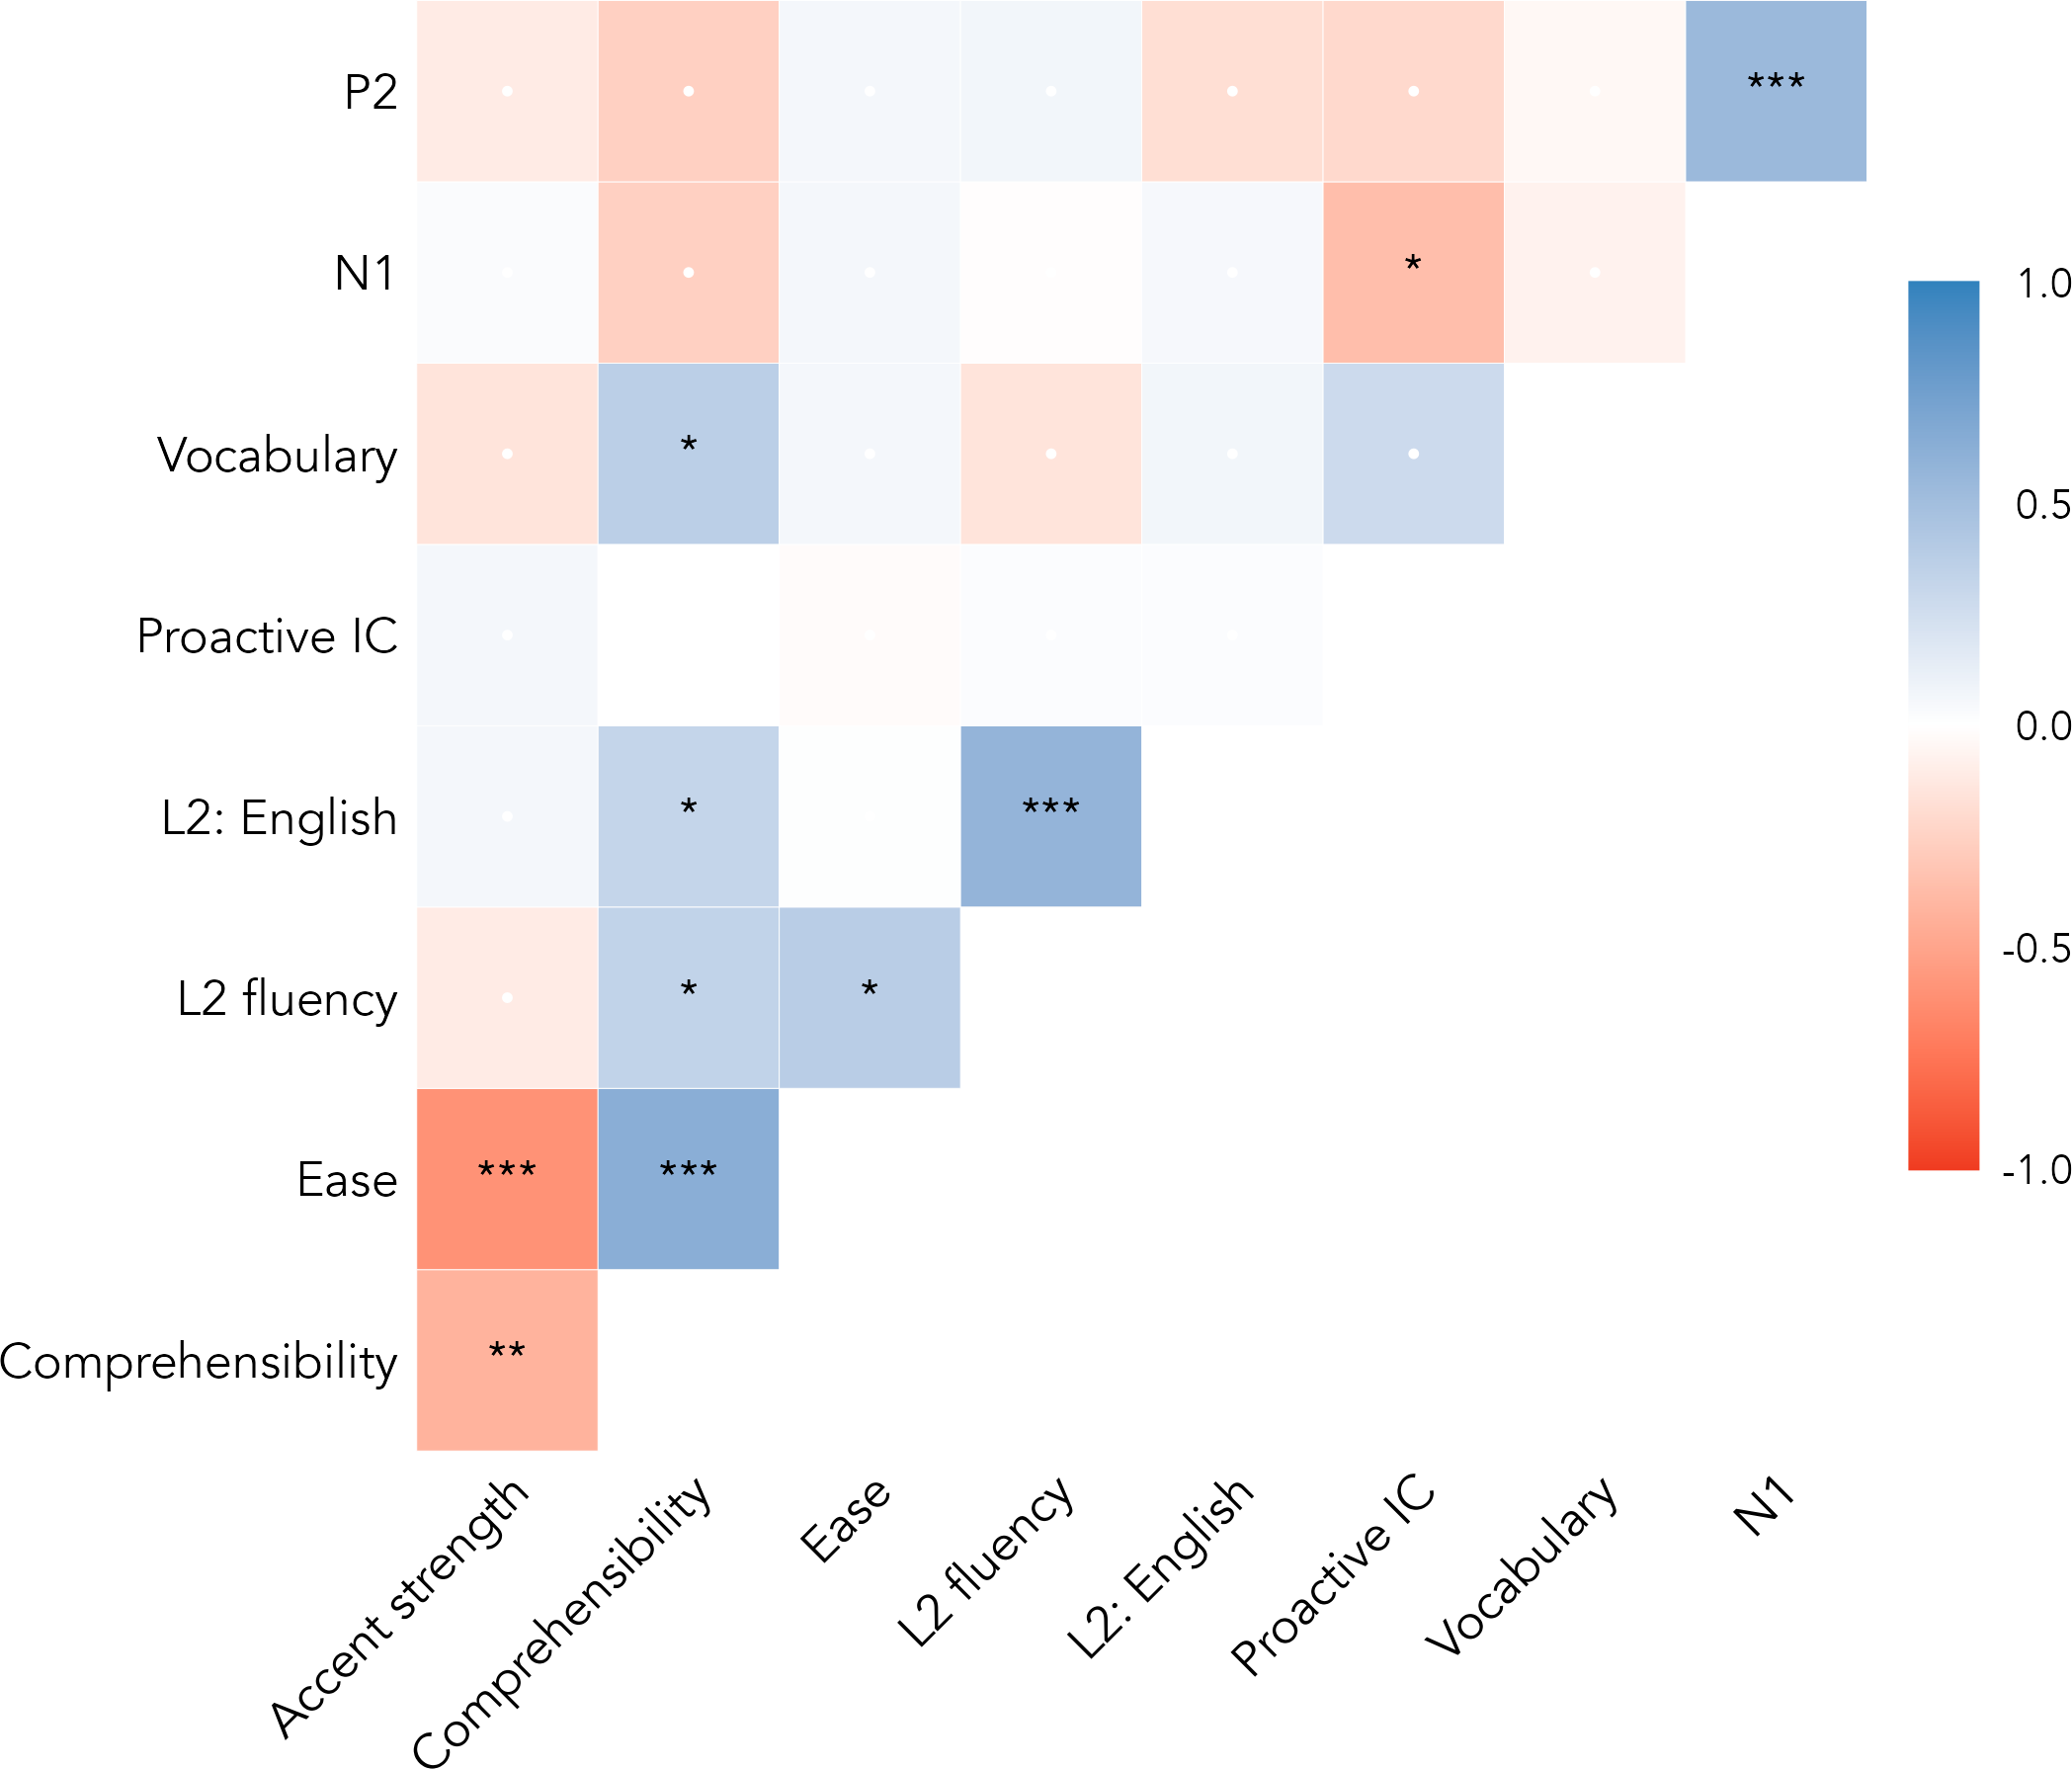
\includegraphics[width=\textwidth]{sections/code/outputs/corr_plot_2} 

}

\caption{Correlation matrix between task performance and post-experiment questionnaire items.}\label{fig:erp-corr-fig}
\end{figure}

Of particular interest is the negative correlation between proactive IC and the magnitude of the N1 priming effect (\emph{r}(38) = -0.36, \emph{p} = .021), with smaller differences between matching and mismatching primes associated with better response inhibition.
This relation suggests that the AX-CPT and LDT share a common inhibitory control mechanism.
We also observed a positive correlation between receptive vocabulary and comprehensibility ratings (\emph{r}(36) = 0.37, \emph{p} = .023), with higher LexTALE scores associated with more confidence in task performance.
Overall, the results of the correlation analysis highlight the influence of more general cognitive/linguistic abilities on task performance.

\hypertarget{discussion-3}{%
\subsection{Discussion}\label{discussion-3}}

The current study investigated the neurocognitive correlates of talker-specific adaptation to L2-accented speech.
We compared two proposed loci of perceptual adaptation: acoustic-phonetic and lexico-semantic.
Behavioral work has shown that listeners adapt to L2-accented talkers by re-tuning their phonetic categories (Reinisch \& Holt, 2014; Xie et al., 2017; Xie \& Myers, 2017).
Theoretical (Goldinger, 1998; Pierrehumbert, 2016; e.g., Sumner et al., 2014) and computational (Kleinschmidt, 2019; Kleinschmidt \& Jaeger, 2015) models of speech perception also identify the acoustic-phonetic level of processing as the site of adaptation.
By contrast, neurocognitive work has observed changes in lexico-semantic access with exposure to L2-accented speech (Romero-Rivas et al., 2015).
More broadly, ERP studies comparing L1- and L2-accented speech have shown that listeners consistently exhibit larger N400 effects for L2 talkers (e.g., Gosselin et al., 2021).
In our study, we observed differences in VOT encoding on the N1 and in phonetic categorization on the P2, which emerged as differences in priming on the N400 disappeared.
Our results provide strongest support for acoustic-phonetic-driven adaptation to L2-accented speech.

\hypertarget{behavioral-adaptation}{%
\subsubsection{Behavioral adaptation}\label{behavioral-adaptation}}

At the behavioral level, listeners exhibited perceptual adaptation to Spanish-accented /p/, /t/, and /k/ as a function of exposure.
Cross-language transfer in Spanish-accented English shortens the VOTs for voiceless stops (Flege \& Eefting, 1987), which makes them perceptually confusible with voiced stops (Chodroff et al., 2019; Lisker \& Abramson, 1970).
In a perceptual adaptation paradigm (Xie et al., 2017; Xie \& Myers, 2017), we exposed listeners to ambiguous voiceless stop onsets in the context of multisyllabic real words (e.g., \emph{passage}).
We probed the status of the adaptation process with monosyllabic real words that have voiced stop onset competitors (e.g., \emph{park}-\emph{bark}).
To investigate learning in real time, we measured accuracy on a primed cross-modal go/no-go lexical decision task (LDT).
First, we compared performance on the Test targets with ambiguous onsets to performance on the Filler targets with unambiguous onsets.
Performance was analyzed in relation to the cumulative amount of experience with Exposure targets with ambiguous onsets in disambiguating lexical contexts.
Performance increased at a faster rate for Test targets versus Filler targets, indicating that the Exposure targets facilitated perceptual adaptation to Spanish-accented voiceless stop onsets.
Second, we compared performance on the Test targets in relation to the three prime types: Identity, Competitor, and Unrelated.
Priming effects did not change with exposure, with accuracy on targets following Competitor primes consistently between Identity and Unrelated primes.

The results of these behavioral analyses suggest that lexically-guided perceptual re-tuning of Spanish-accented voiceless stops had differential effects on high-level categorization versus low-level perception.
Phonetic categorization behavior for voiceless stops did not change throughout the experiment, as evidenced by the main effect of Prime that did not interact with Exposure.
Similarly, the mean error rates in Xie et al. (2017) did not differ between participants with exposure to the critical cue-category mapping and participants with control exposure.
This suggests that high-level categorization behavior is not sufficiently sensitive to priming effects.
However, overall perception of voiceless stops did improve with experience, such that Test target accuracy increased at a higher rate than Filler target accuracy.
Increasing exposure to multisyllabic words with /p/, /t/, and /k/ onsets increased recognition of monosyllabic words with these same onsets.
By contrast, recognition of multisyllabic words with different onsets did not increase at the same rate.
Together, these results suggest that changes in low-level perception of Spanish-accented voiceless stops facilitated word recognition.

\hypertarget{neurocognitive-adaptation}{%
\subsubsection{Neurocognitive adaptation}\label{neurocognitive-adaptation}}

At the neurocognitive level, listeners exhibited fine-grained changes in perception with increasing exposure to Spanish-accented /p/, /t/, and /k/.
The ERP analyses focused on the differential effects of prime type on Test targets.
These analyses were conducted in three time windows: 175-250 ms, 250-375 ms, and 450-650 ms.
These time windows correspond to the N1, P2, and N400 components, respectively.
Building on the ideal adapter framework, we predicted that changes in Competitor primes would constitute evidence for perceptual adaptation.
Specifically, Competitor primes were expected to behave like Identity primes at the beginning of the experiment, when perceptual ambiguity between voiced and voiceless stops was maximal.
By the end of the experiment, Competitor primes were expected to diverge from Identity primes and pattern with the Unrelated primes, since Competitor and Unrelated primes are both mismatches for the target.
This pattern of results was observed most strongly on the N1 component.
During the initial stages of adaptation, Unrelated primes were significantly different from Identity and Competitor primes, which did not differ from one another.
During the later stages of adaptation, the N1 displayed graded sensitivity to prime type, with Unrelated and Competitor primes eliciting more positive responses.
By contrast, Identity primes continued to elicit similarly negative responses on the N1.
These results are broadly consistent with those of Sarrett et al. (2020), who demonstrated an interaction between semantic bias and encoding of ambiguous VOTs.
For example, in a sentence like ``The state fruit of Georgia is the \_\_\_'' (Sarrett et al., 2020), there is a strong semantic bias toward categorizing the ambiguous onset of the final word {[}?i\textipa{\textteshlig}{]} as a /p/ (\emph{peach}) rather than as a /b/ (\emph{beach}).
N1 amplitudes were reduced (less negative) in these voiceless-biased contexts compared to voiced-biased contexts, suggesting more /p/-like encoding of ambiguous VOTs.
In our study, responses to voiceless stop targets were reduced over time in neutral and voiced-biased contexts, suggesting more voiceless-like encoding of ambiguous VOTs with exposure.
Taken together, these results provide support for the prediction following from the ideal adapter framework: namely, that low-level acoustic-phonetic processes support adaptation to L2-accented speech.

An unexpected finding was that responses to Unrelated primes exhibited the largest changes with exposure.
In all three time windows, we observed greater shifts in processing test targets like \emph{park} after primes like \emph{wand}, particularly compared to primes like \emph{park}.
On the N1, these shifts were consistent with increasing perception of short lag VOTs as voiceless stops after Unrelated primes.
We also observed this shift with Competitor primes in line with our predictions for acoustic-phonetic processing; however, Unrelated primes exhibited the highest rate of change.
Moreover, Unrelated primes ultimately elicited the least negative responses to the Test targets.
These findings can be explained by the behavioral data, where we observed the lowest overall accuracy for Unrelated prime trials.
This means that participants had the most room for growth on this trial type compared to the other two.
Previous research suggests that there is a ``Goldilocks zone'' for perceptual adaptation, in which maximally ambiguous tokens that fall between typical and atypical productions exhibit the greatest gains in performance (Babel et al., 2019).
In our study, the Unrelated prime type appears to have landed in this optimal zone for learning at the neurocognitive level.
We were not able to analyze RTs for the priming effects in this task, where Test targets were no-go trials; however, we would also expect a faster rate of growth for Unrelated prime performance based on the ERP data.

On the P2 and N400, the changes in priming were consistent with reductions in processing difficulty for Unrelated primes.
First, we consider the P2, where responses to Unrelated primes decreased in negativity throughout the task.
Larger P2 amplitudes are associated with easier extraction of acoustic-phonetic information from the speech signal (Crowley \& Colrain, 2004).
In addition, changes in P2 amplitude have been associated with successful rule-learning (Diego Balaguer et al., 2007; Rossi et al., 2013; Tong et al., 2009).
According to the ideal adapter framework, listeners use their experience with a talker to update their generative models for particular phonetic categories over acoustic cues (Kleinschmidt \& Jaeger, 2015).
Together, this suggests that exposure to Spanish-accented speech helped listeners update their cue-category mappings between short lag VOTs and voiceless stops.
Turning to the N400, responses to Unrelated primes also decreased in negativity throughout the task, converging with responses to Competitor and Identity primes.
In Romero-Rivas et al. (2015), a reduction in the N400 response to semantically expected words embedded in L2-accented sentences between experiment halves was interpreted as an adaptation effect.
This was in contrast to the P200 response Romero-Rivas et al. (2015) observed, which remained consistently higher for the L1-accented talker than for the L2-accented talker.
Our results suggest that the reduction in the N400 response to Unrelated primes is a product of adaptation at earlier stages of processing.
As the N400 effect in our experiment decreased, sensitivity to the voicing contrast emerged on the N1 and updates to VOT-stop representations emerged on the P2.
Taken together, perceptual adaptation to L2-accented speech appears to be driven by increasing sensitivity to the cue-category mappings that characterize a talker's accent.

\hypertarget{conclusion-1}{%
\subsubsection{Conclusion}\label{conclusion-1}}

This study is among the first to systematically examine the neural signatures associated with adaptation to accented speech.
In behavior, listeners show remarkable speed and plasticity in adjusting to L2-accented speech (Clarke \& Garrett, 2004; Xie et al., 2018).
Our results show that these changes in behavior are supported by changes in specific neurocognitive mechanisms.
In particular, we found that exposure shifted the differential responses of the N1-P2 complex to priming.
The N1 reflected changes in the encoding of VOT as an acoustic cue to voicing, while the P2 reflected changes in the relations between this cue and the phonetic categories /p/, /t/, and /k/.
These results not only provide the first neurocognitive evidence for the ideal adapter framework (Kleinschmidt, 2019; Kleinschmidt \& Jaeger, 2015), but also suggest that changes in acoustic-phonetic linguistic representations drive adaptation (Xie et al., 2023).

\newpage

\hypertarget{general-conclusion}{%
\section{General conclusion}\label{general-conclusion}}

\hypertarget{summary-2}{%
\subsection{Summary}\label{summary-2}}

This dissertation investigated adaptation to L2-accented speech.
Spanish-accented voiceless stop VOT was the focus of the experimental manipulations.
Due to cross-language transfer from Spanish to English in production, the voiceless stops /p/, /t/, and /k/ can be perceptually confusable with their voiced counterparts /b/, /d/, and /g/.
The ambiguity between voiced and voiceless stop pairs in Spanish-accented English is based on their VOT distributions.
L1 English listeners tend to associate short lag VOTs with voiced stops, while Spanish-accented English talkers tend to produce short lag VOTs for voiceless stops.
In order to adapt to Spanish-accented productions of voiceless stops, listeners must learn to associate short lag VOTs with a different set of phonetic categories.
The ideal adapter framework provides useful conceptual tools for investigating this process (Kleinschmidt, 2019; Kleinschmidt \& Jaeger, 2015).
This framework posits that listeners use statistical learning to update generative models of the distributions of phonetic categories over acoustic cues.
I used the ideal adapter framework to answer the following questions: Does increased covariation during exposure enhance talker-independent adaptation beyond exposure-test similarity (Study 1)? Does covariation along one cue-category mapping facilitate generalization to related mappings (Study 1)? What are the relative contributions of phonetic and semantic levels of processing to perceptual adaptation (Study 2)?

\hypertarget{does-increased-covariation-during-exposure-enhance-talker-independent-adaptation-beyond-exposure-test-similarity}{%
\subsection{Does increased covariation during exposure enhance talker-independent adaptation beyond exposure-test similarity?}\label{does-increased-covariation-during-exposure-enhance-talker-independent-adaptation-beyond-exposure-test-similarity}}

The results of Study 1 (Chapter 2) suggest that \emph{decreased} covariation in conjunction with exposure-test similarity enhances talker-independent adaptation.
In Experiment 2, we found that Direct-Invariant exposure reduced the activation of lexical competitors relative to Indirect-Invariant exposure in terms of accuracy on the matching task.
In Experiment 3, Direct-Invariant exposure also reduced lexical competition relative to both the Test-only group and Direct-Invariant exposure in terms of RT on the primed cross-modal lexical decision task.
In both cases, we did not observe any evidence that Variant exposure benefited test performance.
In fact, we found evidence that Invariant exposure actually improved generalization.
There were two explanations for this finding: (1) the talker-independent generative models that listeners developed with Variant exposure were not as useful as the talker-specific generative models that listeners developed with Invariant exposure (2) listeners developed talker-specific generative models regardless of variability, which led to sub-optimal representations of Variant exposure.
Both of these accounts would be consistent with exposure to different VOT distributions for each talker.
To investigate talker-specific VOT-stop distributions, Figure \ref{fig:spk-vot-fig} plots the density of each talker's VOT values across the Direct and Indirect real words from the exposure phase.
Focusing on the voiceless stops encountered during Direct exposure (second row), we can see that the VOT distributions varied by both talker and place of articulation.
This variation is illustrated by comparing both the means and shapes of each distribution, particularly for /p/ (bottom left panel).
Since Direct-Invariant exposure associated each place of articulation with only one talker, listeners did not need to keep track of talkers and places of articulation separately; rather, these sources of variation were collapsed.
Overall, our results suggest that limiting the sources of variation in L2-accented speech facilitates adaptation to specific cue-category mappings.
In terms of the ideal adapter framework, these findings suggest that developing talker-specific generative models for multiple talkers may be the best approach when between-talker and between-category variability is high.

\begin{figure}[H]

{\centering 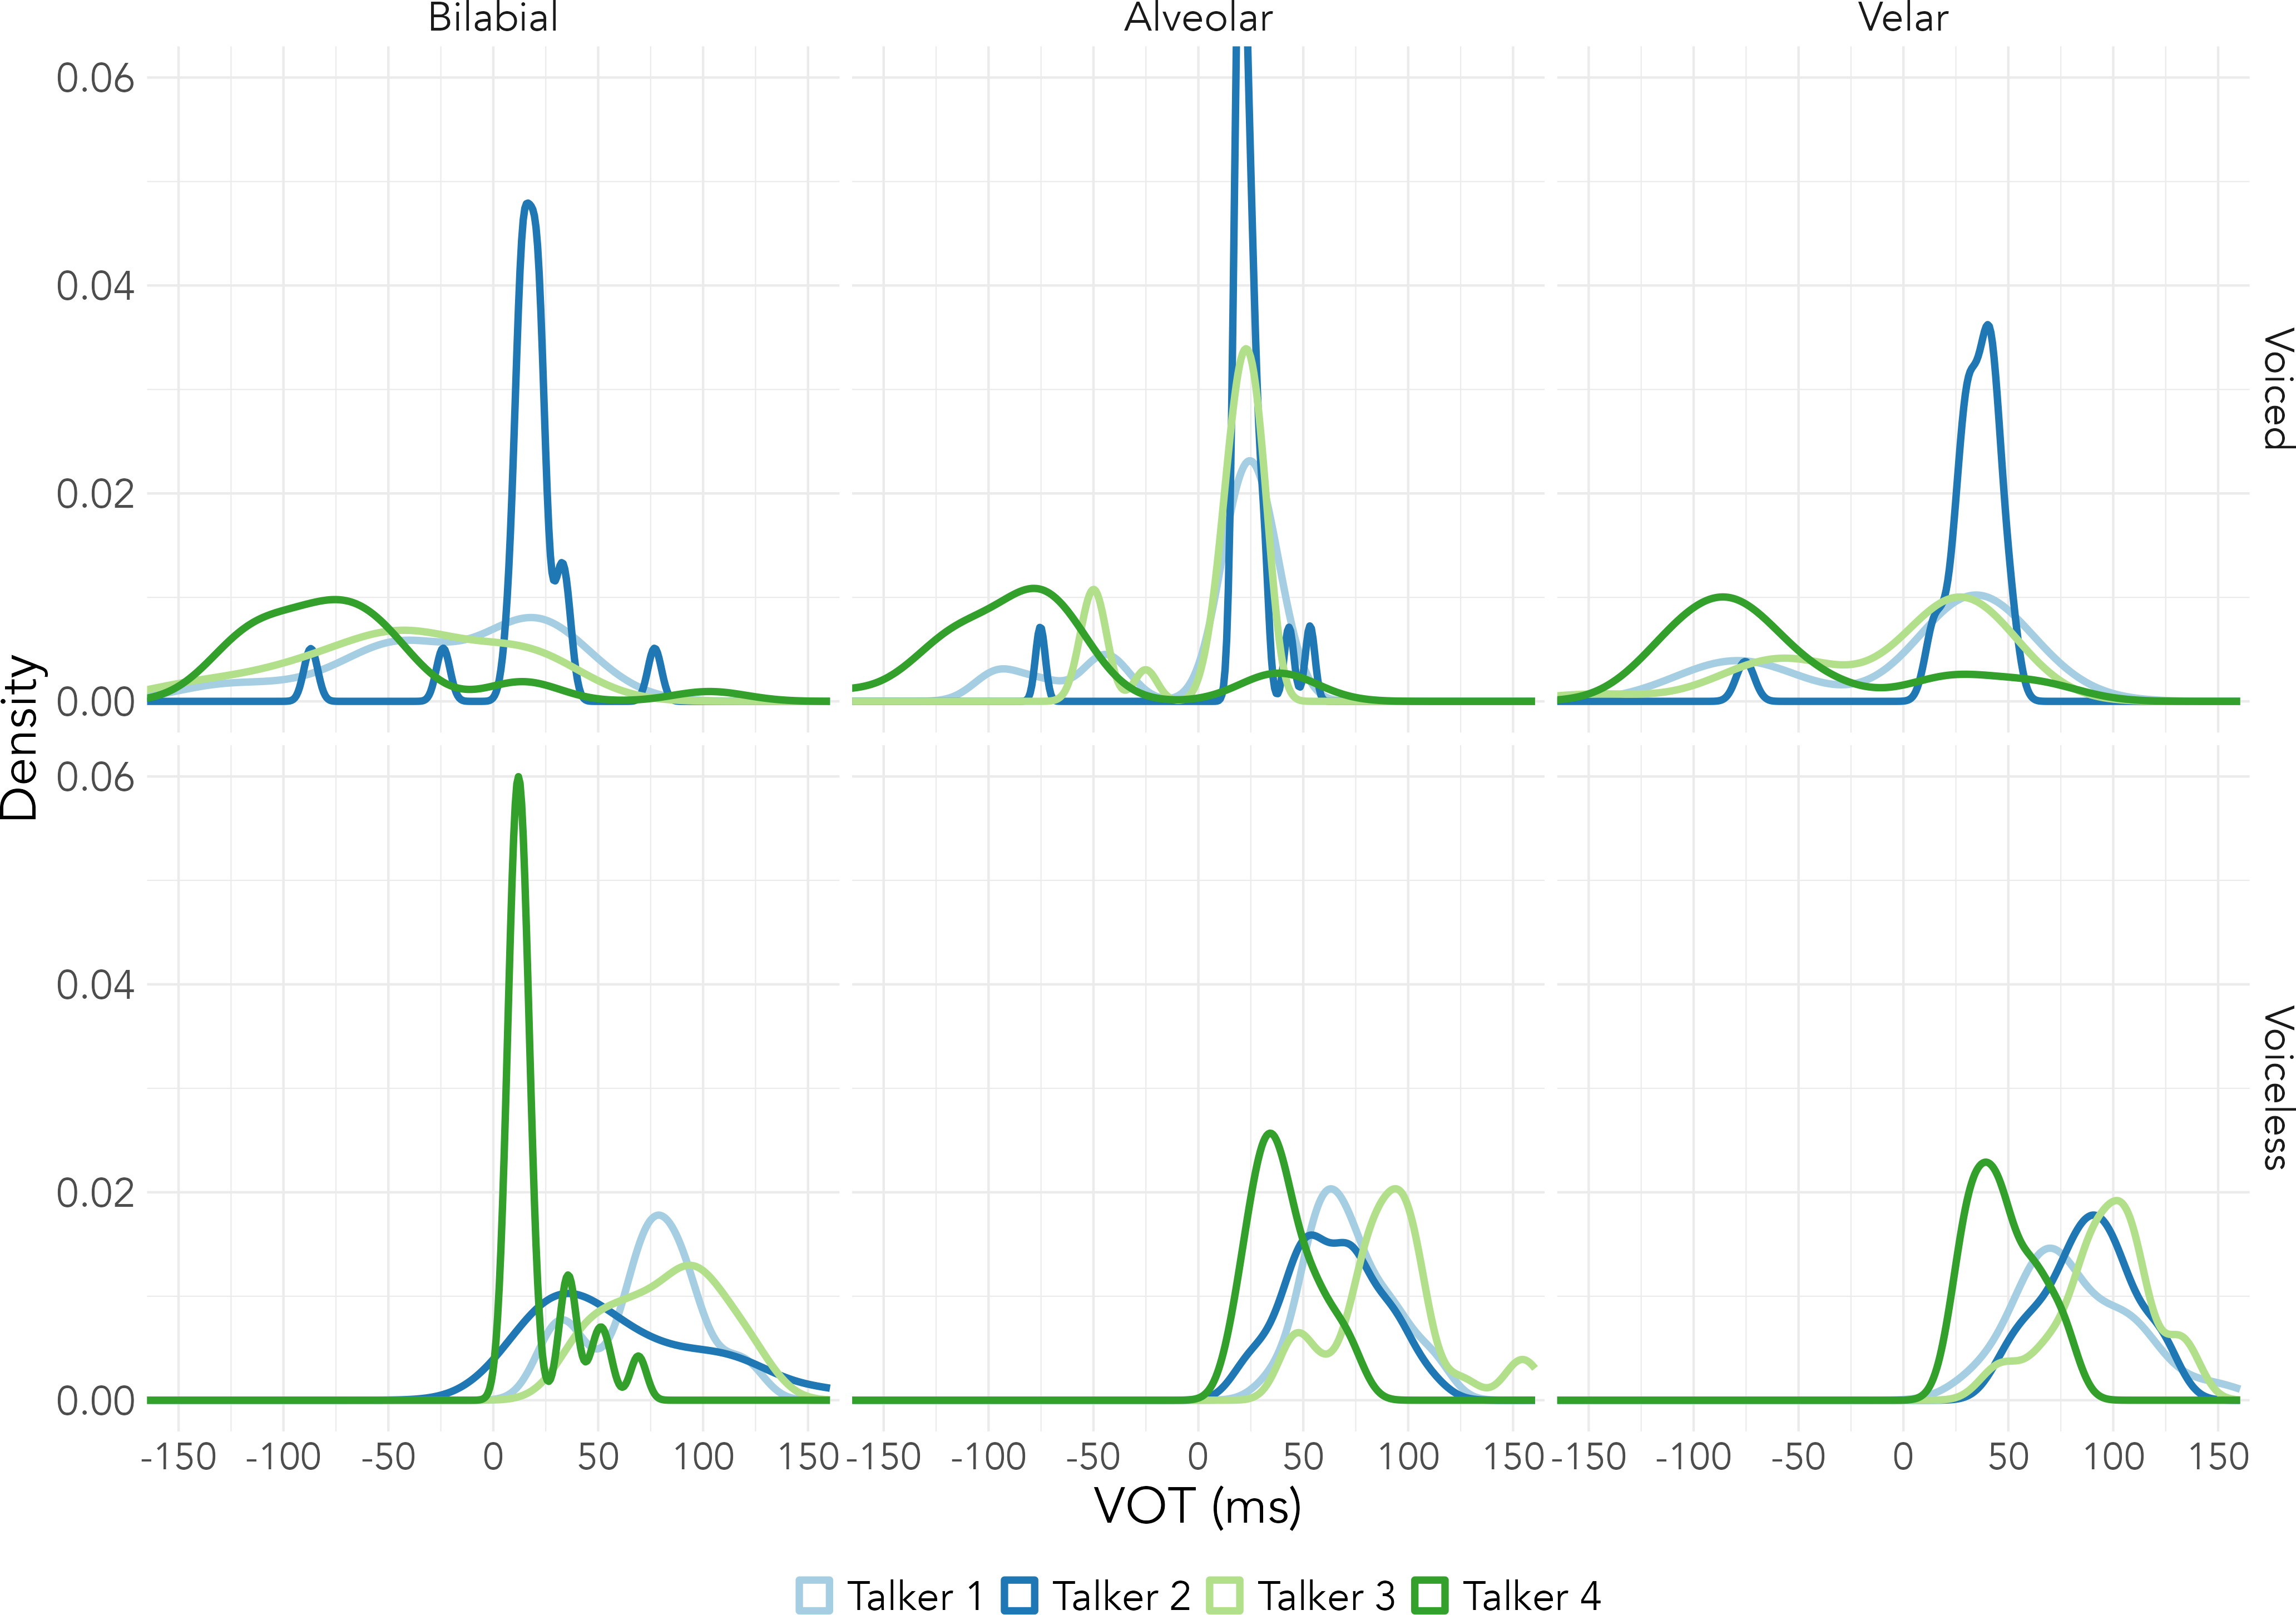
\includegraphics[width=\textwidth]{figures/spk_voice_plot} 

}

\caption{Exposure VOT distributions by talker, place of articulation, and voicing.}\label{fig:spk-vot-fig}
\end{figure}

\hypertarget{does-covariation-along-one-cue-category-mapping-facilitate-generalization-to-related-mappings}{%
\subsection{Does covariation along one cue-category mapping facilitate generalization to related mappings?}\label{does-covariation-along-one-cue-category-mapping-facilitate-generalization-to-related-mappings}}

The results of Study 1 (Chapter 2) suggest that covariation in VOT-voiced stop mappings generalizes to VOT-voiceless stop mappings.
Specifically, in Experiment 3, Indirect-Invariant exposure increased the activation of lexical targets relative to Direct-Invariant exposure in terms of RT on the primed cross-modal lexical decision task.
This finding was unexpected based on previous research and the ideal adapter framework, because it relies on indirect evidence for shifted VOT distributions.
In Indirect conditions, listeners were exposed to lead VOTs in supporting lexical contexts (e.g., \emph{beehive}).
Exposure to these atypical distributions (for L1-accented English) shifted the representations of the VOT distributions for voiced stops from short lag to lead.
In turn, this leftward shift in VOTs for voiced stops triggered a leftward shift in VOTs for voiceless stops, moving the distribution from long lag to short lag.

Considering Figure \ref{fig:spk-vot-fig}, we can see that the VOT distributions for Talkers 1-3's voiceless stops are more short lag than long lag.
The prevalence of these relatively English-like VOT values disrupts the logic of this argument for shifting distributions; an L1 listener's existing generative models of VOT-voiceless stop distributions would be sufficient for categorization.
If listeners did not strictly \emph{need} to adapt, then why did we observe adaptation effects?
One possibility is the presence of an overall L2 accent beyond stop production.
Across the 648 participants in Experiments 1-3, all but nine indicated that the test talker had an accent.
Moreover, more than 90\% of participants identified the test talker as a bilingual.
The talkers' L2-accented features may have encouraged listeners to develop new generative models according to this socio-indexical information (Kleinschmidt, 2019).
Furthermore, development may have been enhanced by exposure to the shifted VOT distributions for voiced stops.
Another possibility is that the shift in VOTs for voiced stops prompted listeners to re-weight the acoustic cues to voicing (Clayards, 2017; Crinnion et al., 2024; Shultz et al., 2012; Toscano \& McMurray, 2010).
That is, instead of using VOT as the primary cue, listeners may have begun to use secondary cues like fundamental frequency.
Updating cue weights may have then benefited perception of voiceless stops during test.

\hypertarget{what-are-the-relative-contributions-of-phonetic-and-semantic-levels-of-processing-to-perceptual-adaptation}{%
\subsection{What are the relative contributions of phonetic and semantic levels of processing to perceptual adaptation?}\label{what-are-the-relative-contributions-of-phonetic-and-semantic-levels-of-processing-to-perceptual-adaptation}}

The experiments in Study 1 (Chapter 2) investigated talker-independent adaptation to Spanish-accented speech.
The experiment in Study 2 (Chapter 3) focused on talker-specific adaptation.
The goal was to investigate the relative contributions of acoustic-phonetic and lexico-semantic levels of processing.
In behavioral paradigms, exposure to a talker's cue-category mappings during exposure facilitates perception of the same talker during test compared to a different talker.
In neurocognitive paradigms, adaptation is not typically the primary focus; as a result, effects of perceptual adaptation on neural signatures are less clear.
We observed differences in VOT perception on the N1 and in phonetic categorization on the P2, which emerged as differences in priming on the N400 disappeared.
The changes we observed in response to Unrelated primes on the N1-P2 complex highlight the role of selective attention in adaptation.
Previous ERP research has shown that the N1-P2 complex reflects the deployment of attention to specific aspects of the speech signal (Hillyard et al., 1973; Joos et al., 2014; Sanders \& Astheimer, 2008).
Previous behavioral work on perceptual adaptation has also demonstrated a link between these two constructs (Francis et al., 2008; Kim et al., 2020; Tzeng et al., 2024).
It is possible that the reduction in N400 effects reflects a shift in attention from the visual prime to the actual speech signal.

\hypertarget{limitations-and-future-directions}{%
\subsection{Limitations and future directions}\label{limitations-and-future-directions}}

Based on theories of L1-L2 transfer in the language system, we assumed that the mean stop VOTs produced by Spanish-accented talkers would be Spanish-like.
That is, we assumed that voiceless stops would be likely to have short lag VOTs and voiced stops would be likely to have lead VOTs.
When we calculated the VOTs produced by our four talkers, we found that voiced stop VOTs were generally Spanish-like, but voiceless stop VOTs were not (see Figure \ref{fig:spk-vot-fig}).
In Study 1 (Chapter 2), the reduction in ambiguity between voiced and voiceless stops reduced the need for adaptation at all, which is likely why performance in the Test-only condition did not differ greatly from performance in any of the exposure conditions.
Another aspect of the stimuli that is worth noting is the difference in VOT distributions between voiced and voiceless stops.
As Figure \ref{fig:spk-vot-fig} shows, the range of VOT values for voiced stops was nearly twice as wide as the range for voiceless stops.
Moreover, the shapes of the distributions were quite different.
Voiceless stop VOTs were more normally distributed (with the exception of Talker 4's distribution for /p/), while voiced stop VOTs varied by talker and place of articulation.
In Study 2 (Chapter 3), Talker 4's voiceless stop VOTs were shortened by 25\% to bring them more fully into the short lag range; however, the shape of the distribution was not altered.
Future iterations of Studies 1 and 2 could both reduce the mean VOTs and change the shape of the VOT distributions to further investigate how cue-category variability influences adaptation.

\hypertarget{conclusion-2}{%
\subsection{Conclusion}\label{conclusion-2}}

Across four experiments, this dissertation explored both talker-specific and talker-independent adaptation to Spanish-accented speech.
VOT provided a window into the adaptation process in both brain and behavior.
The results of the two studies highlight the flexibility of the perceptual system.
The results also support the idea that changes in acoustic-phonetic representations drive adaption.

\FloatBarrier
\newpage

\section*{References}

\setlength{\parindent}{-0.2in}
\setlength{\leftskip}{0.2in}

\noindent

\hypertarget{refs}{}
\begin{CSLReferences}{1}{0}
\leavevmode\vadjust pre{\hypertarget{ref-abramson2017}{}}%
Abramson, A.S., \& Whalen, D.H. (2017). Voice onset time ({VOT}) at 50: Theoretical and practical issues in measuring voicing distinctions. \emph{Journal of Phonetics}, \emph{63}, 75--86.

\leavevmode\vadjust pre{\hypertarget{ref-alexander2019}{}}%
Alexander, J.E.D., \& Nygaard, L.C. (2019). Specificity and generalization in perceptual adaptation to accented speech. \emph{The Journal of the Acoustical Society of America}, \emph{145}(6), 3382--3398.

\leavevmode\vadjust pre{\hypertarget{ref-andruski1994}{}}%
Andruski, J.E., Blumstein, S.E., \& Burton, M. (1994). The effect of subphonetic differences on lexical access. \emph{Cognition}, \emph{52}(3), 163--187.

\leavevmode\vadjust pre{\hypertarget{ref-atienza2002}{}}%
Atienza, M., Cantero, J.L., \& Dominguez-Marin, E. (2002). The time course of neural changes underlying auditory perceptual learning. \emph{Learning \& Memory}, \emph{9}(3), 138--150.

\leavevmode\vadjust pre{\hypertarget{ref-babel2019}{}}%
Babel, M., McAuliffe, M., Norton, C., Senior, B., \& Vaughn, C. (2019). The {Goldilocks} zone of perceptual learning. \emph{Phonetica}, \emph{76}(2-3), 179--200.

\leavevmode\vadjust pre{\hypertarget{ref-baese2013}{}}%
Baese-Berk, M.M., Bradlow, A.R., \& Wright, B.A. (2013). Accent-independent adaptation to foreign accented speech. \emph{The Journal of the Acoustical Society of America}, \emph{133}(3), EL174--EL180.

\leavevmode\vadjust pre{\hypertarget{ref-baigorri2019}{}}%
Baigorri, M., Campanelli, L., \& Levy, E.S. (2019). Perception of {American}--{English} vowels by early and late {Spanish}--{English} bilinguals. \emph{Language and Speech}, \emph{62}(4), 681--700.

\leavevmode\vadjust pre{\hypertarget{ref-balota2007}{}}%
Balota, D.A., Yap, M.J., Hutchison, K.A., Cortese, M.J., Kessler, B., Loftis, B., Neely, J.H., Nelson, D.L., Simpson, G.B., \& Treiman, R. (2007). The {English} lexicon project. \emph{Behavior Research Methods}, \emph{39}, 445--459.

\leavevmode\vadjust pre{\hypertarget{ref-banks2015}{}}%
Banks, B., Gowen, E., Munro, K.J., \& Adank, P. (2015). Cognitive predictors of perceptual adaptation to accented speech. \emph{The Journal of the Acoustical Society of America}, \emph{137}(4), 2015--2024.

\leavevmode\vadjust pre{\hypertarget{ref-barr2013}{}}%
Barr, D.J., Levy, R., Scheepers, C., \& Tily, H.J. (2013). Random effects structure for confirmatory hypothesis testing: Keep it maximal. \emph{Journal of Memory and Language}, \emph{68}(3), 255--278.

\leavevmode\vadjust pre{\hypertarget{ref-bates2015}{}}%
Bates, D., Mächler, M., Bolker, B., \& Walker, S. (2015). Fitting linear mixed-effects models using {lme4}. \emph{Journal of Statistical Software}, \emph{67}(1), 1--48. \url{https://doi.org/10.18637/jss.v067.i01}

\leavevmode\vadjust pre{\hypertarget{ref-benki2001}{}}%
Benkí, J.R. (2001). Place of articulation and first formant transition pattern both affect perception of voicing in {English}. \emph{Journal of Phonetics}, \emph{29}(1), 1--22.

\leavevmode\vadjust pre{\hypertarget{ref-bent2021}{}}%
Bent, T., \& Baese-Berk, M. (2021). \emph{Perceptual learning of accented speech} (J. S. Pardo, L. C. Nygaard, R. E. Remez, \& D. B. Pisoni, Eds.; pp. 428--464). Wiley Blackwell.

\leavevmode\vadjust pre{\hypertarget{ref-best1994}{}}%
Best, C.T. (1994). The emergence of native-language phonological influences in infants: A perceptual assimilation model. \emph{The Development of Speech Perception: The Transition from Speech Sounds to Spoken Words}, \emph{167}(224), 233--277.

\leavevmode\vadjust pre{\hypertarget{ref-best2001}{}}%
Best, C.T., McRoberts, G.W., \& Goodell, E. (2001). Discrimination of non-native consonant contrasts varying in perceptual assimilation to the listener's native phonological system. \emph{The Journal of the Acoustical Society of America}, \emph{109}(2), 775--794.

\leavevmode\vadjust pre{\hypertarget{ref-best2007}{}}%
Best, C.T., \& Tyler, M. (2007). \emph{Second language speech learning: The role of language experience in speech perception and production} (O. Bohn \& M. Munro, Eds.; pp. 13--34). John Benjamins.

\leavevmode\vadjust pre{\hypertarget{ref-bieber2022}{}}%
Bieber, R.E., \& Gordon-Salant, S. (2022). Semantic context and stimulus variability independently affect rapid adaptation to non-native english speech in young adults. \emph{The Journal of the Acoustical Society of America}, \emph{151}(1), 242--255.

\leavevmode\vadjust pre{\hypertarget{ref-blakesley2009}{}}%
Blakesley, R.E., Mazumdar, S., Dew, M.A., Houck, P.R., Tang, G., Reynolds III, C.F., \& Butters, M.A. (2009). Comparisons of methods for multiple hypothesis testing in neuropsychological research. \emph{Neuropsychology}, \emph{23}(2), 255.

\leavevmode\vadjust pre{\hypertarget{ref-bradlow2023}{}}%
Bradlow, A.R., Bassard, A.M., \& Paller, K.A. (2023). Generalized perceptual adaptation to second-language speech: Variability, similarity, and intelligibility. \emph{The Journal of the Acoustical Society of America}, \emph{154}(3), 1601--1613.

\leavevmode\vadjust pre{\hypertarget{ref-bradlow2008}{}}%
Bradlow, A.R., \& Bent, T. (2008). Perceptual adaptation to non-native speech. \emph{Cognition}, \emph{106}(2), 707--729.

\leavevmode\vadjust pre{\hypertarget{ref-broersma2021}{}}%
Broersma, P., \& Weenink, D. (2021). \emph{Praat: Doing phonetics by computer} (Version 6.1.38). \url{http://www.praat.org/}

\leavevmode\vadjust pre{\hypertarget{ref-brunelliere2013}{}}%
Brunellière, A., \& Soto-Faraco, S. (2013). The speakers' accent shapes the listeners' phonological predictions during speech perception. \emph{Brain and Language}, \emph{125}(1), 82--93.

\leavevmode\vadjust pre{\hypertarget{ref-brysbaert2019}{}}%
Brysbaert, M., Mandera, P., McCormick, S.F., \& Keuleers, E. (2019). Word prevalence norms for 62,000 {English} lemmas. \emph{Behavior Research Methods}, \emph{51}, 467--479.

\leavevmode\vadjust pre{\hypertarget{ref-campos2012}{}}%
Campos-Astorkiza, R. (2012). The phonemes of {Spanish}. \emph{The Handbook of Hispanic Linguistics}, 89--110.

\leavevmode\vadjust pre{\hypertarget{ref-chatrian1985}{}}%
Chatrian, G.E., Lettich, E., \& Nelson, P.L. (1985). Ten percent electrode system for topographic studies of spontaneous and evoked EEG activities. \emph{American Journal of EEG Technology}, \emph{25}(2), 83--92.

\leavevmode\vadjust pre{\hypertarget{ref-cho1999}{}}%
Cho, T., \& Ladefoged, P. (1999). Variation and universals in {VOT}: Evidence from 18 languages. \emph{Journal of Phonetics}, \emph{27}(2), 207--229.

\leavevmode\vadjust pre{\hypertarget{ref-chodroff2019}{}}%
Chodroff, E., Golden, A., \& Wilson, C. (2019). Covariation of stop voice onset time across languages: Evidence for a universal constraint on phonetic realization. \emph{The Journal of the Acoustical Society of America}, \emph{145}(1), EL109--EL115.

\leavevmode\vadjust pre{\hypertarget{ref-chodroff2017}{}}%
Chodroff, E., \& Wilson, C. (2017). Structure in talker-specific phonetic realization: Covariation of stop consonant {VOT in American English}. \emph{Journal of Phonetics}, \emph{61}, 30--47.

\leavevmode\vadjust pre{\hypertarget{ref-choi2019}{}}%
Choi, J.Y., \& Perrachione, T.K. (2019). Time and information in perceptual adaptation to speech. \emph{Cognition}, \emph{192}, 103982.

\leavevmode\vadjust pre{\hypertarget{ref-clarke2004}{}}%
Clarke, C.M., \& Garrett, M.F. (2004). Rapid adaptation to foreign-accented {English}. \emph{The Journal of the Acoustical Society of America}, \emph{116}(6), 3647--3658.

\leavevmode\vadjust pre{\hypertarget{ref-clarke2005}{}}%
Clarke, C.M., \& Luce, P. (2005). Perceptual adaptation to speaker characteristics: {VOT} boundaries in stop voicing categorization. \emph{ISCA Workshop on Plasticity in Speech Perception}.

\leavevmode\vadjust pre{\hypertarget{ref-clayards2017}{}}%
Clayards, M. (2017). Individual talker and token covariation in the production of multiple cues to stop voicing. \emph{Phonetica}, \emph{75}(1), 1--23.

\leavevmode\vadjust pre{\hypertarget{ref-clayards2008}{}}%
Clayards, M., Tanenhaus, M.K., Aslin, R.N., \& Jacobs, R.A. (2008). Perception of speech reflects optimal use of probabilistic speech cues. \emph{Cognition}, \emph{108}(3), 804--809.

\leavevmode\vadjust pre{\hypertarget{ref-connolly1994}{}}%
Connolly, J.F., \& Phillips, N.A. (1994). Event-related potential components reflect phonological and semantic processing of the terminal word of spoken sentences. \emph{Journal of Cognitive Neuroscience}, \emph{6}(3), 256--266.

\leavevmode\vadjust pre{\hypertarget{ref-cooper1974}{}}%
Cooper, W.E. (1974). Selective adaptation for acoustic cues of voicing in initial stops. \emph{Journal of Phonetics}, \emph{2}(4), 303--313.

\leavevmode\vadjust pre{\hypertarget{ref-crinnion2024}{}}%
Crinnion, A.M., Luthra, S., Gaston, P., \& Magnuson, J.S. (2024). Resolving competing predictions in speech: How qualitatively different cues and cue reliability contribute to phoneme identification. \emph{Attention, Perception, \& Psychophysics}, 1--20.

\leavevmode\vadjust pre{\hypertarget{ref-crowley2004}{}}%
Crowley, K.E., \& Colrain, I.M. (2004). A review of the evidence for {P2} being an independent component process: Age, sleep and modality. \emph{Clinical Neurophysiology}, \emph{115}(4), 732--744.

\leavevmode\vadjust pre{\hypertarget{ref-cummings2023}{}}%
Cummings, S.N., \& Theodore, R.M. (2023). Hearing is believing: Lexically guided perceptual learning is graded to reflect the quantity of evidence in speech input. \emph{Cognition}, \emph{235}, 105404.

\leavevmode\vadjust pre{\hypertarget{ref-delorme2004}{}}%
Delorme, A., \& Makeig, S. (2004). {EEGLAB}: An open source toolbox for analysis of single-trial {EEG} dynamics including independent component analysis. \emph{Journal of Neuroscience Methods}, \emph{134}(1), 9--21.

\leavevmode\vadjust pre{\hypertarget{ref-desroches2009}{}}%
Desroches, A.S., Newman, R.L., \& Joanisse, M.F. (2009). Investigating the time course of spoken word recognition: Electrophysiological evidence for the influences of phonological similarity. \emph{Journal of Cognitive Neuroscience}, \emph{21}(10), 1893--1906.

\leavevmode\vadjust pre{\hypertarget{ref-dediego2007}{}}%
Diego Balaguer, R. de, Toro, J.M., Rodriguez-Fornells, A., \& Bachoud-Lévi, A.-C. (2007). Different neurophysiological mechanisms underlying word and rule extraction from speech. \emph{PLoS One}, \emph{2}(11), e1175.

\leavevmode\vadjust pre{\hypertarget{ref-dorman1974}{}}%
Dorman, M.F. (1974). Auditory evoked potential correlates of speech sound discrimination. \emph{Perception \& Psychophysics}, \emph{15}, 215--220.

\leavevmode\vadjust pre{\hypertarget{ref-eisner2005}{}}%
Eisner, F., \& McQueen, J.M. (2005). The specificity of perceptual learning in speech processing. \emph{Perception \& Psychophysics}, \emph{67}(2), 224--238.

\leavevmode\vadjust pre{\hypertarget{ref-elangovan2011}{}}%
Elangovan, S., \& Stuart, A. (2011). A cross-linguistic examination of cortical auditory evoked potentials for a categorical voicing contrast. \emph{Neuroscience Letters}, \emph{490}(2), 140--144.

\leavevmode\vadjust pre{\hypertarget{ref-ethnologue2024_2}{}}%
Ethnologue. (2024). \emph{What are the top 200 most spoken languages?} \url{https://www.ethnologue.com/insights/ethnologue200/}

\leavevmode\vadjust pre{\hypertarget{ref-federmeier2021}{}}%
Federmeier, K.D. (2021). Connecting and considering: Electrophysiology provides insights into comprehension. \emph{Psychophysiology}, e13940.

\leavevmode\vadjust pre{\hypertarget{ref-flege2007}{}}%
Flege, J.E. (2007). Language contact in bilingualism: Phonetic system interactions. \emph{Laboratory Phonology}, \emph{9}(353-381).

\leavevmode\vadjust pre{\hypertarget{ref-flege2021}{}}%
Flege, J.E., \& Bohn, O. (2021). The revised speech learning model (SLM-r). \emph{Second Language Speech Learning: Theoretical and Empirical Progress}, 3--83.

\leavevmode\vadjust pre{\hypertarget{ref-flege1987}{}}%
Flege, J.E., \& Eefting, W. (1987). Production and perception of english stops by native spanish speakers. \emph{Journal of Phonetics}, \emph{15}(1), 67--83.

\leavevmode\vadjust pre{\hypertarget{ref-flege2003}{}}%
Flege, J.E., Schirru, C., \& MacKay, I.R.A. (2003). Interaction between the native and second language phonetic subsystems. \emph{Speech Communication}, \emph{40}(4), 467--491.

\leavevmode\vadjust pre{\hypertarget{ref-fox2019}{}}%
Fox, J., \& Weisberg, S. (2019). \emph{An {R} companion to applied regression} (Third). Sage. \url{https://socialsciences.mcmaster.ca/jfox/Books/Companion/}

\leavevmode\vadjust pre{\hypertarget{ref-francis2008}{}}%
Francis, A.L., Kaganovich, N., \& Driscoll-Huber, C. (2008). Cue-specific effects of categorization training on the relative weighting of acoustic cues to consonant voicing in english. \emph{The Journal of the Acoustical Society of America}, \emph{124}(2), 1234--1251.

\leavevmode\vadjust pre{\hypertarget{ref-getz2019}{}}%
Getz, L.M., \& Toscano, J.C. (2019). Electrophysiological evidence for top-down lexical influences on early speech perception. \emph{Psychological Science}, \emph{30}(6), 830--841.

\leavevmode\vadjust pre{\hypertarget{ref-getz2021}{}}%
Getz, L.M., \& Toscano, J.C. (2021). The time-course of speech perception revealed by temporally-sensitive neural measures. \emph{Wiley Interdisciplinary Reviews: Cognitive Science}, \emph{12}(2), e1541.

\leavevmode\vadjust pre{\hypertarget{ref-goldinger1998}{}}%
Goldinger, S.D. (1998). Echoes of echoes? An episodic theory of lexical access. \emph{Psychological Review}, \emph{105}(2), 251.

\leavevmode\vadjust pre{\hypertarget{ref-goslin2012}{}}%
Goslin, J., Duffy, H., \& Floccia, C. (2012). An {ERP} investigation of regional and foreign accent processing. \emph{Brain and Language}, \emph{122}(2), 92--102.

\leavevmode\vadjust pre{\hypertarget{ref-gosselin2021}{}}%
Gosselin, L., Martin, C.D., Navarra-Barindelli, E., \& Caffarra, S. (2021). The presence of a foreign accent introduces lexical integration difficulties during late semantic processing. \emph{Language, Cognition and Neuroscience}, 1--21.

\leavevmode\vadjust pre{\hypertarget{ref-grey2017}{}}%
Grey, S., \& Van Hell, J.G. (2017). Foreign-accented speaker identity affects neural correlates of language comprehension. \emph{Journal of Neurolinguistics}, \emph{42}, 93--108.

\leavevmode\vadjust pre{\hypertarget{ref-hagoort2017}{}}%
Hagoort, P. (2017). The core and beyond in the language-ready brain. \emph{Neuroscience \& Biobehavioral Reviews}, \emph{81}, 194--204.

\leavevmode\vadjust pre{\hypertarget{ref-hanulikova2012}{}}%
Hanulíková, A., Van Alphen, P.M., Van Goch, M.M., \& Weber, A. (2012). When one person's mistake is another's standard usage: The effect of foreign accent on syntactic processing. \emph{Journal of Cognitive Neuroscience}, \emph{24}(4), 878--887.

\leavevmode\vadjust pre{\hypertarget{ref-hillyard1973}{}}%
Hillyard, S.A., Hink, R.F., Schwent, V.L., \& Picton, T.W. (1973). Electrical signs of selective attention in the human brain. \emph{Science}, \emph{182}(4108), 177--180.

\leavevmode\vadjust pre{\hypertarget{ref-horev2007}{}}%
Horev, N., Most, T., \& Pratt, H. (2007). Categorical perception of speech ({VOT}) and analogous non-speech ({FOT}) signals: Behavioral and electrophysiological correlates. \emph{Ear and Hearing}, \emph{28}(1), 111--128.

\leavevmode\vadjust pre{\hypertarget{ref-huang2020}{}}%
Huang, X.-J., Yang, J.-C., et al. (2020). Phonological {P2 or PMN} during spoken word recognition in {Mandarin Chinese}: Prime modality matters. \emph{Journal of Psychophysiology}, \emph{34}(2).

\leavevmode\vadjust pre{\hypertarget{ref-hubert2008}{}}%
Hubert, M., \& Vandervieren, E. (2008). An adjusted boxplot for skewed distributions. \emph{Computational Statistics \& Data Analysis}, \emph{52}(12), 5186--5201.

\leavevmode\vadjust pre{\hypertarget{ref-idemaru2011}{}}%
Idemaru, K., \& Holt, L.L. (2011). Word recognition reflects dimension-based statistical learning. \emph{Journal of Experimental Psychology: Human Perception and Performance}, \emph{37}(6), 1939.

\leavevmode\vadjust pre{\hypertarget{ref-johnson2006}{}}%
Johnson, K. (2006). Resonance in an exemplar-based lexicon: The emergence of social identity and phonology. \emph{Journal of Phonetics}, \emph{34}(4), 485--499.

\leavevmode\vadjust pre{\hypertarget{ref-joos2014}{}}%
Joos, K., Gilles, A., Van de Heyning, P., De Ridder, D., \& Vanneste, S. (2014). From sensation to percept: The neural signature of auditory event-related potentials. \emph{Neuroscience \& Biobehavioral Reviews}, \emph{42}, 148--156.

\leavevmode\vadjust pre{\hypertarget{ref-kang2024}{}}%
Kang, O., Yan, X., Kostromitina, M., Thomson, R., \& Isaacs, T. (2024). Fairness of using different english accents: The effect of shared L1s in listening tasks of the duolingo english test. \emph{Language Testing}, \emph{41}(2), 263--289.

\leavevmode\vadjust pre{\hypertarget{ref-kapnoula2021}{}}%
Kapnoula, E.C., \& McMurray, B. (2021). Idiosyncratic use of bottom-up and top-down information leads to differences in speech perception flexibility: Converging evidence from ERPs and eye-tracking. \emph{Brain and Language}, \emph{223}, 105031.

\leavevmode\vadjust pre{\hypertarget{ref-kim2020}{}}%
Kim, D., Clayards, M., \& Kong, E.J. (2020). Individual differences in perceptual adaptation to unfamiliar phonetic categories. \emph{Journal of Phonetics}, \emph{81}, 100984.

\leavevmode\vadjust pre{\hypertarget{ref-kleinschmidt2019}{}}%
Kleinschmidt, D.F. (2019). Structure in talker variability: How much is there and how much can it help? \emph{Language, Cognition and Neuroscience}, \emph{34}(1), 43--68.

\leavevmode\vadjust pre{\hypertarget{ref-kleinschmidt2015}{}}%
Kleinschmidt, D.F., \& Jaeger, T.F. (2015). Robust speech perception: Recognize the familiar, generalize to the similar, and adapt to the novel. \emph{Psychological Review}, \emph{122}(2), 148.

\leavevmode\vadjust pre{\hypertarget{ref-kraljic2006}{}}%
Kraljic, T., \& Samuel, A.G. (2006). Generalization in perceptual learning for speech. \emph{Psychonomic Bulletin \& Review}, \emph{13}(2), 262--268.

\leavevmode\vadjust pre{\hypertarget{ref-kraljic2007}{}}%
Kraljic, T., \& Samuel, A.G. (2007). Perceptual adjustments to multiple speakers. \emph{Journal of Memory and Language}, \emph{56}(1), 1--15.

\leavevmode\vadjust pre{\hypertarget{ref-kutas1984}{}}%
Kutas, M., \& Hillyard, S.A. (1984). Brain potentials during reading reflect word expectancy and semantic association. \emph{Nature}, \emph{307}(5947), 161--163.

\leavevmode\vadjust pre{\hypertarget{ref-lemhofer2012}{}}%
Lemhöfer, K., \& Broersma, M. (2012). Introducing {LexTALE}: A quick and valid lexical test for advanced learners of english. \emph{Behavior Research Methods}, \emph{44}, 325--343.

\leavevmode\vadjust pre{\hypertarget{ref-lenth2022}{}}%
Lenth, R.V. (2022). \emph{Emmeans: Estimated marginal means, aka least-squares means}. \url{https://CRAN.R-project.org/package=emmeans}

\leavevmode\vadjust pre{\hypertarget{ref-lewendon2023}{}}%
Lewendon, J., Britton, J., \& Politzer-Ahles, S. (2023). The MMN by another name? Exploring the autonomy of the phonological mapping (mismatch) negativity. \emph{Language, Cognition and Neuroscience}, \emph{38}(8), 1098--1114.

\leavevmode\vadjust pre{\hypertarget{ref-lewendon2020}{}}%
Lewendon, J., Mortimore, L., \& Egan, C. (2020). The phonological mapping (mismatch) negativity: History, inconsistency, and future direction. \emph{Frontiers in Psychology}, \emph{11}, 1967.

\leavevmode\vadjust pre{\hypertarget{ref-lisker1970}{}}%
Lisker, L., \& Abramson, A.S. (1970). The voicing dimension: Some experiments in comparative phonetics. \emph{Proceedings of the 6th International Congress of Phonetic Sciences}, 563--567.

\leavevmode\vadjust pre{\hypertarget{ref-lisker1964}{}}%
Lisker, L., \& Abramson, A.S. (1964). A cross-language study of voicing in initial stops: Acoustical measurements. \emph{Word}, \emph{20}(3), 384--422.

\leavevmode\vadjust pre{\hypertarget{ref-luck2014}{}}%
Luck, S.J. (2014). \emph{An introduction to the event-related potential technique}. MIT press.

\leavevmode\vadjust pre{\hypertarget{ref-lukacs2023}{}}%
Lukács, G., Kawai, C., Ansorge, U., \& Fekete, A. (2023). Detecting concealed language knowledge via response times. \emph{Applied Linguistics Review}, \emph{14}(4), 1027--1044.

\leavevmode\vadjust pre{\hypertarget{ref-luthra2021}{}}%
Luthra, S., Mechtenberg, H., \& Myers, E.B. (2021). Perceptual learning of multiple talkers requires additional exposure. \emph{Attention, Perception, \& Psychophysics}, \emph{83}, 2217--2228.

\leavevmode\vadjust pre{\hypertarget{ref-malins2012}{}}%
Malins, J.G., \& Joanisse, M.F. (2012). Setting the tone: An {ERP} investigation of the influences of phonological similarity on spoken word recognition in mandarin chinese. \emph{Neuropsychologia}, \emph{50}(8), 2032--2043.

\leavevmode\vadjust pre{\hypertarget{ref-marslen1984}{}}%
Marslen-Wilson, W.D. (1984). Function and process in spoken word recognition: A tutorial review. \emph{Attention and Performance: Control of Language Processes}, 125--150.

\leavevmode\vadjust pre{\hypertarget{ref-mcclelland1986}{}}%
McClelland, J.L., \& Elman, J.L. (1986). The {TRACE} model of speech perception. \emph{Cognitive Psychology}, \emph{18}(1), 1--86.

\leavevmode\vadjust pre{\hypertarget{ref-mccullough2016}{}}%
McCullough, E.A., \& Clopper, C.G. (2016). Perceptual subcategories within non-native {English}. \emph{Journal of Phonetics}, \emph{55}, 19--37.

\leavevmode\vadjust pre{\hypertarget{ref-morales2015}{}}%
Morales, J., Yudes, C., Gómez-Ariza, C.J., \& Bajo, M.T. (2015). Bilingualism modulates dual mechanisms of cognitive control: Evidence from ERPs. \emph{Neuropsychologia}, \emph{66}, 157--169.

\leavevmode\vadjust pre{\hypertarget{ref-nagle2022}{}}%
Nagle, C.L., \& Baese-Berk, M.M. (2022). Advancing the state of the art in L2 speech perception-production research: Revisiting theoretical assumptions and methodological practices. \emph{Studies in Second Language Acquisition}, \emph{44}(2), 580--605.

\leavevmode\vadjust pre{\hypertarget{ref-newman2009}{}}%
Newman, R.L., \& Connolly, J.F. (2009). Electrophysiological markers of pre-lexical speech processing: Evidence for bottom--up and top--down effects on spoken word processing. \emph{Biological Psychology}, \emph{80}(1), 114--121.

\leavevmode\vadjust pre{\hypertarget{ref-norris1994}{}}%
Norris, D. (1994). Shortlist: A connectionist model of continuous speech recognition. \emph{Cognition}, \emph{52}(3), 189--234.

\leavevmode\vadjust pre{\hypertarget{ref-norris2003}{}}%
Norris, D., McQueen, J.M., \& Cutler, A. (2003). Perceptual learning in speech. \emph{Cognitive Psychology}, \emph{47}(2), 204--238.

\leavevmode\vadjust pre{\hypertarget{ref-oldfield1971}{}}%
Oldfield, R.C. (1971). The assessment and analysis of handedness: The edinburgh inventory. \emph{Neuropsychologia}, \emph{9}(1), 97--113.

\leavevmode\vadjust pre{\hypertarget{ref-peirce2019}{}}%
Peirce, J., Gray, J.R., Simpson, S., MacAskill, M., Höchenberger, R., Sogo, H., Kastman, E., \& Lindeløv, J.K. (2019). PsychoPy2: Experiments in behavior made easy. \emph{Behavior Research Methods}, \emph{51}, 195--203.

\leavevmode\vadjust pre{\hypertarget{ref-pereira2018}{}}%
Pereira, O., Gao, Y.A., \& Toscano, J.C. (2018). Perceptual encoding of natural speech sounds revealed by the N1 event-related potential response. \emph{Auditory Perception \& Cognition}, \emph{1}(1-2), 112--130.

\leavevmode\vadjust pre{\hypertarget{ref-pierrehumbert2016}{}}%
Pierrehumbert, J.B. (2016). Phonological representation: Beyond abstract versus episodic. \emph{Annual Review of Linguistics}, \emph{2}, 33--52.

\leavevmode\vadjust pre{\hypertarget{ref-porretta2017}{}}%
Porretta, V., Tremblay, A., \& Bolger, P. (2017). Got experience? PMN amplitudes to foreign-accented speech modulated by listener experience. \emph{Journal of Neurolinguistics}, \emph{44}, 54--67.

\leavevmode\vadjust pre{\hypertarget{ref-port1982}{}}%
Port, R.F., \& Dalby, J. (1982). Consonant/vowel ratio as a cue for voicing in english. \emph{Perception \& Psychophysics}, \emph{32}, 141--152.

\leavevmode\vadjust pre{\hypertarget{ref-rcore2022}{}}%
R Core Team. (2022). \emph{R: A language and environment for statistical computing}. R Foundation for Statistical Computing. \url{https://www.R-project.org/}

\leavevmode\vadjust pre{\hypertarget{ref-ramautar2004}{}}%
Ramautar, J., Kok, A., \& Ridderinkhof, K. (2004). Effects of stop-signal probability in the stop-signal paradigm: The {N2/P3} complex further validated. \emph{Brain and Cognition}, \emph{56}(2), 234--252.

\leavevmode\vadjust pre{\hypertarget{ref-reinisch2014}{}}%
Reinisch, E., \& Holt, L.L. (2014). Lexically guided phonetic retuning of foreign-accented speech and its generalization. \emph{Journal of Experimental Psychology: Human Perception and Performance}, \emph{40}(2), 539.

\leavevmode\vadjust pre{\hypertarget{ref-revelle2023}{}}%
Revelle, W. (2023). \emph{Psych: Procedures for psychological, psychometric, and personality research}. Northwestern University. \url{https://CRAN.R-project.org/package=psych}

\leavevmode\vadjust pre{\hypertarget{ref-romerorivas2015}{}}%
Romero-Rivas, C., Martin, C.D., \& Costa, A. (2015). Processing changes when listening to foreign-accented speech. \emph{Frontiers in Human Neuroscience}, \emph{9}, 167.

\leavevmode\vadjust pre{\hypertarget{ref-rossi2013}{}}%
Rossi, S., Hartmüller, T., Vignotto, M., \& Obrig, H. (2013). Electrophysiological evidence for modulation of lexical processing after repetitive exposure to foreign phonotactic rules. \emph{Brain and Language}, \emph{127}(3), 404--414.

\leavevmode\vadjust pre{\hypertarget{ref-sanders2008}{}}%
Sanders, L.D., \& Astheimer, L.B. (2008). Temporally selective attention modulates early perceptual processing: Event-related potential evidence. \emph{Perception \& Psychophysics}, \emph{70}(4), 732--742.

\leavevmode\vadjust pre{\hypertarget{ref-sarrett2020}{}}%
Sarrett, M.E., McMurray, B., \& Kapnoula, E.C. (2020). Dynamic {EEG} analysis during language comprehension reveals interactive cascades between perceptual processing and sentential expectations. \emph{Brain and Language}, \emph{211}, 104875.

\leavevmode\vadjust pre{\hypertarget{ref-scharenborg2019}{}}%
Scharenborg, O., Koemans, J., Smith, C., Hasegawa-Johnson, M.A., \& Federmeier, K.D. (2019). The neural correlates underlying lexically-guided perceptual learning. \emph{INTERSPEECH}, 1223--1227.

\leavevmode\vadjust pre{\hypertarget{ref-schertz2016}{}}%
Schertz, J., Cho, T., Lotto, A., \& Warner, N. (2016). Individual differences in perceptual adaptability of foreign sound categories. \emph{Attention, Perception, \& Psychophysics}, \emph{78}, 355--367.

\leavevmode\vadjust pre{\hypertarget{ref-shultz2012}{}}%
Shultz, A.A., Francis, A.L., \& Llanos, F. (2012). Differential cue weighting in perception and production of consonant voicing. \emph{The Journal of the Acoustical Society of America}, \emph{132}(2), EL95--EL101.

\leavevmode\vadjust pre{\hypertarget{ref-sidaras2009}{}}%
Sidaras, S.K., Alexander, J.E.D., \& Nygaard, L.C. (2009). Perceptual learning of systematic variation in {Spanish-accented} speech. \emph{The Journal of the Acoustical Society of America}, \emph{125}(5), 3306--3316.

\leavevmode\vadjust pre{\hypertarget{ref-song2018}{}}%
Song, J., \& Iverson, P. (2018). Listening effort during speech perception enhances auditory and lexical processing for non-native listeners and accents. \emph{Cognition}, \emph{179}, 163--170.

\leavevmode\vadjust pre{\hypertarget{ref-stringer2019}{}}%
Stringer, L., \& Iverson, P. (2019). Accent intelligibility differences in noise across native and nonnative accents: Effects of talker--listener pairing at acoustic--phonetic and lexical levels. \emph{Journal of Speech, Language, and Hearing Research}, \emph{62}(7), 2213--2226.

\leavevmode\vadjust pre{\hypertarget{ref-sumner2014}{}}%
Sumner, M., Kim, S.K., King, E., \& McGowan, K.B. (2014). The socially weighted encoding of spoken words: A dual-route approach to speech perception. \emph{Frontiers in Psychology}, \emph{4}, 1015.

\leavevmode\vadjust pre{\hypertarget{ref-tong2009}{}}%
Tong, Y., Melara, R.D., \& Rao, A. (2009). P2 enhancement from auditory discrimination training is associated with improved reaction times. \emph{Brain Research}, \emph{1297}, 80--88.

\leavevmode\vadjust pre{\hypertarget{ref-toscanomc2010}{}}%
Toscano, J.C., \& McMurray, B. (2010). Cue integration with categories: Weighting acoustic cues in speech using unsupervised learning and distributional statistics. \emph{Cognitive Science}, \emph{34}(3), 434--464.

\leavevmode\vadjust pre{\hypertarget{ref-toscano2010}{}}%
Toscano, J.C., McMurray, B., Dennhardt, J., \& Luck, S.J. (2010). Continuous perception and graded categorization: Electrophysiological evidence for a linear relationship between the acoustic signal and perceptual encoding of speech. \emph{Psychological Science}, \emph{21}(10), 1532--1540.

\leavevmode\vadjust pre{\hypertarget{ref-tremblay2001}{}}%
Tremblay, K., Kraus, N., McGee, T., Ponton, C., Otis, B., et al. (2001). Central auditory plasticity: Changes in the {N1}--{P2} complex after speech-sound training. \emph{Ear and Hearing}, \emph{22}(2), 79--90.

\leavevmode\vadjust pre{\hypertarget{ref-tyler2014}{}}%
Tyler, M.D., Best, C.T., Faber, A., \& Levitt, A.G. (2014). Perceptual assimilation and discrimination of non-native vowel contrasts. \emph{Phonetica}, \emph{71}(1), 4--21.

\leavevmode\vadjust pre{\hypertarget{ref-tzeng2016}{}}%
Tzeng, C.Y., Alexander, J.E.D., Sidaras, S.K., \& Nygaard, L.C. (2016). The role of training structure in perceptual learning of accented speech. \emph{Journal of Experimental Psychology: Human Perception and Performance}, \emph{42}(11), 1793.

\leavevmode\vadjust pre{\hypertarget{ref-tzeng2024}{}}%
Tzeng, C.Y., Russell, M.L., \& Nygaard, L.C. (2024). Attention modulates perceptual learning of non-native-accented speech. \emph{Attention, Perception, \& Psychophysics}, \emph{86}(1), 339--353.

\leavevmode\vadjust pre{\hypertarget{ref-un2024}{}}%
United Nations. (2024). \emph{Standard country or area codes for statistical use (M49)}. \url{https://unstats.un.org/unsd/methodology/m49/}

\leavevmode\vadjust pre{\hypertarget{ref-utman2000}{}}%
Utman, J.A., Blumstein, S.E., \& Burton, M.W. (2000). Effects of subphonetic and syllable structure variation on word recognition. \emph{Perception \& Psychophysics}, \emph{62}, 1297--1311.

\leavevmode\vadjust pre{\hypertarget{ref-vicente1986}{}}%
Vicente, M.L.C. (1986). El {VOT} de las oclusivas sordas y sonoras espa{ñ}olas. \emph{Estudios de Fon{é}tica Experimental}, 91--110.

\leavevmode\vadjust pre{\hypertarget{ref-viswanathan2020}{}}%
Viswanathan, N., Olmstead, A.J., \& Aivar, M.P. (2020). The use of vowel length in making voicing judgments by native listeners of {English and Spanish}: Implications for rate normalization. \emph{Language and Speech}, \emph{63}(2), 436--452.

\leavevmode\vadjust pre{\hypertarget{ref-wade2007}{}}%
Wade, T., Jongman, A., \& Sereno, J. (2007). Effects of acoustic variability in the perceptual learning of non-native-accented speech sounds. \emph{Phonetica}, \emph{64}(2-3), 122--144.

\leavevmode\vadjust pre{\hypertarget{ref-whalen1993}{}}%
Whalen, D.H., Abramson, A.S., Lisker, L., \& Mody, M. (1993). F0 gives voicing information even with unambiguous voice onset times. \emph{The Journal of the Acoustical Society of America}, \emph{93}(4), 2152--2159.

\leavevmode\vadjust pre{\hypertarget{ref-whalen2018}{}}%
Whalen, D.H., Chen, W.-R., Tiede, M.K., \& Nam, H. (2018). Variability of articulator positions and formants across nine english vowels. \emph{Journal of Phonetics}, \emph{68}, 1--14.

\leavevmode\vadjust pre{\hypertarget{ref-williams1977}{}}%
Williams, L. (1977). The voicing contrast in {Spanish}. \emph{Journal of Phonetics}, \emph{5}(2), 169--184.

\leavevmode\vadjust pre{\hypertarget{ref-winn2020}{}}%
Winn, M.B. (2020). Manipulation of voice onset time in speech stimuli: A tutorial and flexible praat script. \emph{The Journal of the Acoustical Society of America}, \emph{147}(2), 852--866.

\leavevmode\vadjust pre{\hypertarget{ref-witteman2013}{}}%
Witteman, M.J., Weber, A., \& McQueen, J.M. (2013). Foreign accent strength and listener familiarity with an accent codetermine speed of perceptual adaptation. \emph{Attention, Perception, \& Psychophysics}, \emph{75}(3), 537--556.

\leavevmode\vadjust pre{\hypertarget{ref-woods2017}{}}%
Woods, K.J., Siegel, M.H., Traer, J., \& McDermott, J.H. (2017). Headphone screening to facilitate web-based auditory experiments. \emph{Attention, Perception, \& Psychophysics}, \emph{79}, 2064--2072.

\leavevmode\vadjust pre{\hypertarget{ref-wu2022}{}}%
Wu, Y.C., \& Holt, L.L. (2022). Phonetic category activation predicts the direction and magnitude of perceptual adaptation to accented speech. \emph{Journal of Experimental Psychology: Human Perception and Performance}, \emph{48}(9), 913---925.

\leavevmode\vadjust pre{\hypertarget{ref-xie2020}{}}%
Xie, X., \& Jaeger, T.F. (2020). Comparing non-native and native speech: Are L2 productions more variable? \emph{The Journal of the Acoustical Society of America}, \emph{147}(5), 3322--3347.

\leavevmode\vadjust pre{\hypertarget{ref-xie2023}{}}%
Xie, X., Jaeger, T.F., \& Kurumada, C. (2023). What we do (not) know about the mechanisms underlying adaptive speech perception: A computational framework and review. \emph{Cortex}, \emph{166}, 377--424.

\leavevmode\vadjust pre{\hypertarget{ref-xie2021}{}}%
Xie, X., Liu, L., \& Jaeger, T.F. (2021). Cross-talker generalization in the perception of nonnative speech: A large-scale replication. \emph{Journal of Experimental Psychology: General}.

\leavevmode\vadjust pre{\hypertarget{ref-xie2017similarity}{}}%
Xie, X., \& Myers, E.B. (2017). Learning a talker or learning an accent: Acoustic similarity constrains generalization of foreign accent adaptation to new talkers. \emph{Journal of Memory and Language}, \emph{97}, 30--46.

\leavevmode\vadjust pre{\hypertarget{ref-xie2017structure}{}}%
Xie, X., Theodore, R.M., \& Myers, E.B. (2017). More than a boundary shift: Perceptual adaptation to foreign-accented speech reshapes the internal structure of phonetic categories. \emph{Journal of Experimental Psychology: Human Perception and Performance}, \emph{43}(1), 206.

\leavevmode\vadjust pre{\hypertarget{ref-xie2018}{}}%
Xie, X., Weatherholtz, K., Bainton, L., Rowe, E., Burchill, Z., Liu, L., \& Jaeger, T.F. (2018). Rapid adaptation to foreign-accented speech and its transfer to an unfamiliar talker. \emph{The Journal of the Acoustical Society of America}, \emph{143}(4), 2013--2031.

\leavevmode\vadjust pre{\hypertarget{ref-young2018}{}}%
Young, M.E., Sutherland, S.C., \& McCoy, A.W. (2018). Optimal go/no-go ratios to maximize false alarms. \emph{Behavior Research Methods}, \emph{50}, 1020--1029.

\leavevmode\vadjust pre{\hypertarget{ref-zhang2021hvpt}{}}%
Zhang, X., Cheng, B., \& Zhang, Y. (2021). The role of talker variability in nonnative phonetic learning: A systematic review and meta-analysis. \emph{Journal of Speech, Language, and Hearing Research}, \emph{64}(12), 4802--4825.

\end{CSLReferences}

\end{document}
